\documentclass[a4paper,10pt,twoside]{article}

%Sección de paquetes
\usepackage[utf8]{inputenc}
\usepackage[style=ieee]{biblatex}
\usepackage{csquotes}
\usepackage[top=2.5cm,bottom=2.5cm,left=4cm,right=2cm]{geometry}
\usepackage[spanish,es-tabla]{babel}
\usepackage{float}
\usepackage{caption}
\usepackage{pdfpages} % Para insertar la portada en formato PDF.
\usepackage[hidelinks]{hyperref} % Para urls.
\usepackage{longtable} % Para tablas largas.
\usepackage{graphicx} % Para cargar imagenes
\usepackage{titlesec}
\usepackage{fancyhdr}
\usepackage[parfill]{parskip}
\usepackage[acronym,nogroupskip]{glossaries}
\usepackage{todonotes}
\usepackage{dirtree}
\usepackage{subcaption}
\usepackage{mathtools}
\usepackage{amsmath}
\usepackage{multirow}
\usepackage{algpseudocodex}
\usepackage{algorithm}
\usepackage{listings}
\raggedbottom

\addbibresource{TFGDiego.bib}

%Eliminar la sangría y otros ajustes de los headers
\setlength{\parindent}{0px}
\setlength{\headheight}{13.07225pt}
%Glosarios
\makenoidxglossaries

%ACRONIMOS

\newacronym{fao}{FAO}{Food and Agriculture Organization of the United Nations}
\newacronym{i+d}{I+D}{Investigación y Desarrollo}
\newacronym{ETSIAAB}{ETSIAAB}{Escuela Técnica Superior de Ingeniería Agronómica, Alimentaria y de Biosistemas}
\newacronym{pran}{PRAN}{Grupo de Investigación de Producción Animal}
\newacronym{mts}{MTS}{MPEG Transport Stream}
\newacronym{fps}{FPS}{Frames Per Second}
\newacronym{mov}{MOV}{QuickTime File Format}
\newacronym{ltr}{LTR}{Left To Right}
\newacronym{ocr}{OCR}{Optical Character Recognition}
\newacronym{mlp}{MLP}{MultiLayer Perceptron}
\newacronym{roi}{ROI}{Region Of Interest}
\newacronym{cnn}{CNN}{Convolutional Neural Networks}
\newacronym{map}{mAP}{Mean Average Precision}
\newacronym{citsem}{CITSEM}{Centro de Investigación en Tecnologías Software y Sistemas Multimedia para la Sostenibilidad}
\newacronym{gpu}{GPU}{Graphics Processing Unit}
\newacronym{cpu}{CPU}{Central Processing Unit}
%GLOSARIO Y DEFINICIONES


\renewcommand*\glspostdescription{\hfill}
\newcommand\acrfullr[2][]{\acrshort[#1]{#2} (\acrlong[#1]{#2})}


%Nuevos estilos de páginas por errores
\fancypagestyle{specialpage}{%
  \fancyhf{}
  \fancyhead[R]{\textit{1 LISTA DE ACRÓNIMOS}}
  \fancyfoot[EL]{\thepage}
  \fancyfoot[OR]{\thepage}
}
\fancypagestyle{indicefig}{
  \fancyhf{}
  \fancyhead[L]{\textit{ÍNDICE DE FIGURAS Y TABLAS}}
  \fancyfoot[EL]{\thepage}
  \fancyfoot[OR]{\thepage}
}
\fancypagestyle{abstract}{
    \fancyhf{}
    \renewcommand{\headrulewidth}{0pt} % Asegurarse de que la barra negra también se elimine en esta página
    \fancyfoot[EL]{\thepage}
    \fancyfoot[OR]{\thepage}
}

%Cosas para escribir pseudocodigo
\makeatletter
\def\BState{\State\hskip-\ALG@thistlm}
\makeatother


\title{TFG Diego Aceituno Seoane}
\author{Diego Aceituno Seoane}
\date{Diego Aceituno Seoane}

\begin{document}

\pagenumbering{gobble}
\begin{titlepage}
    
\includepdf[pages=1,offset=0 0, pagecommand={}]{./TFG_Primera Hoja.pdf}
\end{titlepage}

\newpage
\pagenumbering{arabic}
\thispagestyle{abstract}
\begin{flushright}
    \vspace*{5cm}
    \medskip
    Agradezco a  \dots

    Gracias a \dots

    A \dots port \dots
\end{flushright}



\newpage
\thispagestyle{abstract}
\mbox{}
\newpage
\clearpage
\section*{RESUMEN}
\thispagestyle{abstract}
En los últimos años la visión por ordenador ha tomado un papel muy importante en la vida cotidiana. Dentro de este campo encontramos técnicas como el análisis de 
flujo óptico o las redes neuronales de tipo \texttt{CNN}, siendo \texttt{YOLO} una arquitectura muy popular.

En este trabajo se ha desarollado una aplicación de detección y contabilización del número de movimientos realizados por truchas en videos del experimento \textit{NetTest}. 
Para esto se ha formado un conjunto de datos y se ha entrenado un modelo de \texttt{YOLOv8}, el cual procesa el video y devuelve los resultados de las \texttt{Bounding Boxes} 
asociadas a cada trucha.\newline Posteriormente los datos son transformados y se les aplica un algoritmo para estimar los fotogramas en los que ha sucedido un movimiento. 
Encima de esto, se ha desarrollado una interfaz gráfica que realiza todo esto de forma transparente a los conocimientos del usuario. Para implementar todas las funcionalidades 
se han utilizado herramientas como la ejecución paralela y la inferencia de forma transparente al \texttt{HardWare}.

Como resultados, el modelo \texttt{YOLOv8n} se ha entrenado hasta reducir el error asociado a la \texttt{Bounding Box} y maximizar la puntuación \texttt{F1}. Finalmente, la 
comparación de resultados con una serie de datos etiquetados en 64 videos ha demostrado una tasa de error de \texttt{$ \pm 20\% $}.
\newpage
\thispagestyle{abstract}
\mbox{}
\newpage
\section*{ABSTRACT}
\thispagestyle{abstract}
Aquí dentro se introduciría el abstract en Inglés.
\newpage
\thispagestyle{abstract}
\mbox{}
\newpage
\clearpage

%Page numbering and headers para el resto de secciones
\pagestyle{fancy}
\fancyfoot{}
\fancyhead[EL]{}
\fancyhead[OR]{}
\fancyfoot[EL]{\thepage}
\fancyfoot[OR]{\thepage}
\tableofcontents
\clearpage
\thispagestyle{indicefig}
\listoffigures
\thispagestyle{indicefig}
\listoftables

\newpage
\thispagestyle{abstract}
\mbox{}
\newpage
\section{LISTA DE ACRÓNIMOS} % Glosario
\thispagestyle{specialpage}
\printnoidxglossary[style=list,type=\acronymtype,title=] % Acrónimos
\newpage
\thispagestyle{abstract}
\mbox{}
\newpage
\section{INTRODUCCIÓN}

\subsection{Marco y motivación del proyecto}

Las crisis alimenticias afectan a diversas partes del globo, en mayor o menor medida. Estas crisis pueden producirse por factores naturales o factores humanos como, por ejemplo, 
fallos en industrias, guerras, o, la que directamente se relaciona con este proyecto, agotamiento de los recursos naturales por la sobreexplotación.

Ante estas situaciones globales que pasan por revisar los valores de obtención de alimento y el cómo se gestionan los recursos, la pesca marítima está viendo como insostenible la 
compatibilidad de su labor con la generación de suficiente alimento vivo para suplir las necesidades exponenciales del ser humano.

El caso que más afecta a este trabajo es la acuicultura, un método alternativo que nació para obtener control sobre el desarrollo de especies muy difíciles de capturar en entornos 
libres. Esto se consigue a través de crianza controlada en entornos limitados, como piscifactorías o jaulas masivas en costas.

Este método de generación de alimento ha ido desarrollándose y mejorando a través de la introducción de nuevos métodos y tecnologías. Esta mejora ha permitido utilizar la acuicultura 
como principal método de crianza de ciertas especies, que; aun encontrándose en libertad, es más viable económicamente trabajar con ellas en estos entornos controlados. Esto permite liberar 
estrés de los ecosistemas marítimos.

Con estos ecosistemas tan afectados por las pescas de arrastre y, con la presión añadida por políticas limitantes en este ámbito, la pesca tradicional ha visto como la cantidad de alimento 
generado no crece a lo largo de los años. Esto se ve reflejado a través de los informes realizados por la \textit{\acrfull{fao}}, siendo el último en 2022, que marcaba aún más la tendencia del 
impulso hacia sistemas basados en acuicultura, observable en la \autoref{fig:EvolucionFAO}.

\begin{figure}[h]
    \centering
    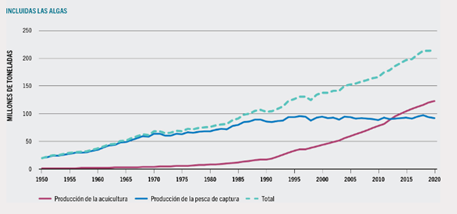
\includegraphics[width=0.75\textwidth]{images/1/EvolucionFAO.png}
    \caption{Evolución de la producción en la industria pesquera 1950-2020}
    \label{fig:EvolucionFAO}
\end{figure}

La acuicultura está representando un cambio de paradigma para proteger nuestros ecosistemas y producir con menos perdidas y de manera más ética. Con esto en mente, se están promoviendo muchos planes de transformación digital en estas industrias, con la inversión en I+D que eso conlleva.

Algunas de las investigaciones que se realizan en este campo tienen relación con el estudio de métodos de crianza que generen menos estrés en el pez. Mejoras en este campo podrían permitir un crecimiento más rápido del alimento vivo aumentando su bienestar y un mejor marco ético en la crianza del animal.

En concreto, para realizar un análisis y parametrizado del estrés del animal, se llevan a cabo diferentes experimentos con el objetivo final de valorar los resultados del cambio de metodologías. Siendo el “Net Test”[2] uno de estos experimentos.

El principal objetivo de este experimento es parametrizar la proactividad de un pez a través de los movimientos que realiza. Junto con este y otros datos del pez como podría ser su color o tamaño, intentar parametrizar y encontrar reglas de como se ha visto afectado por cambios de entorno. Si bien esta prueba no está estandarizada (la definición de movimiento puede variar entre diferentes trabajos académicos), en este trabajo se tratará el caso específico en el que los movimientos contados, son arpeos del espécimen.

En la actualidad esta prueba se realiza de forma manual, siendo necesario que el investigador utilice herramientas de análisis de videos para apuntar cuando se realizan estos movimientos, avanzando fotograma a fotograma. Un ejemplo de este tipo de herramientas son herramientas como BORIS[3].

La existencia de este tipo de herramientas de código abierto es muy positiva para el mundo de la investigación, pero el hecho de tener un funcionamiento completamente manual conlleva un gasto de tiempo y recursos en obtener estos informes de movimientos para cada video.

Con esto en mente se es interesante crear una alternativa que automatice el proceso de conteo para los investigadores que utilizan el NetTest como experimento principal.

\subsection{Objetivos técnicos y académicos}
Los objetivos de este trabajo consisten en:

\begin{enumerate}
    \item Plantear una alternativa capaz de automatizar el NetTest.
    \item Estudiar el uso de tecnologías basadas en procesado y análisis de imagen y técnicas de Deep Learning para implementar esta alternativa
    \item Desarrollar una aplicación completa a través de la alternativa planteada
\end{enumerate}

Los objetivos académicos de este proyecto son:

\begin{enumerate}
    \item Desarrollar una mejor capacidad de análisis de requisitos técnicos a la hora de diseño de aplicaciones.
    \item Profundizar en el entendimiento de técnicas basadas en Deep Learning como las redes neuronales.
    \item Mejorar las aptitudes relacionadas con el análisis de artículos académicos con el objetivo de realizar un estudio del arte suficientemente profundo, cohesionado y coherente con la problemática explicada.
\end{enumerate}


\subsection{Estructura del resto de la memoria}
\section{MARCO TECNOLÓGICO}

El problema que se busca solucionar en este trabajo tiene relación directa con el estudio de la visión por ordenador. Este campo de la Ingeniería busca, 
a través de sistemas de captación y procesamiento de imágenes, generar información y automatizar procesos con ordenadores. \newline Dentro de este área se han desarrollado tecnologías que usamos día a día
\cite{szeliskiComputerVisionAlgorithms2022}:

\begin{itemize}
    \item \textbf{\textit{\acrfullr{ocr}}} para realizar reconocimiento de texto en imágenes y documentos.
    \item \textbf{Detección de fallos en maquinaria} en procesos de fabricación.
    \item \textbf{Fotogrametría} para mapear imágenes a modelos \texttt{3D}.
    \item \textbf{Imagen médica} para uso en operaciones a tiempo real\cite{NEMESIS3DCM}.
    \item \textbf{Detección de objetos} en imágenes o videos.
    \item \textbf{Detección de movimiento} y seguimiento de objetos en escenas.
\end{itemize}

Las aplicaciones que usan herramientas basadas en este tipo de soluciones suelen seguir una estructura similar a la siguiente:

\begin{enumerate}
    \item Capturar información a través de cámaras o flujos de video IP de diferentes características.
    \item (A veces) Realizar un preprocesamiento de las imágenes para adaptarlas al sistema.
    \item Procesar las imágenes para extraer información relevante para el sistema.
    \item Transformar la información extraída a través de algoritmos inteligentes para construir una base de datos que sea útil para el usuario de la aplicación.
\end{enumerate}

En el caso de este trabajo, se tratan problemas de detección de objetos y análisis de cambio. Este tipo de tareas se han llevado a cabo antiguamente a través de algoritmos complejos y deterministas, pero en los últimos 
años, con el auge del aprendizaje automático, se ha creado un nuevo paradigma.

En los siguientes puntos se van a describir de forma breve las técnicas de aprendizaje automático, los sistemas de detección de objetos, seguimiento de cambio y los entornos de desarrollo y despliegue 
de estas técnicas de forma transparente al \texttt{Hardware} disponible así como proyectos relacionados con este trabajo.
\clearpage

\subsection{Aprendizaje Automático y \texttt{Deep Learning}}

\subsubsection{Definición y tipos de tareas}

El campo del aprendizaje automático busca desarrollar soluciones a través de algoritmos y sistemas que permitan a los ordenadores tratar los datos entrantes como el cerebro humano, siendo capaz de 
generalizar las propiedades que les definen y encontrar patrones.

Este aprendizaje automático se realiza sobre un conjunto de datos que aporta el usuario con el objetivo de abstraer diferentes informaciones específicas o agrupar los datos según patrones. Este aprendizaje 
habitualmente se realiza a través de un bucle de tres fases (ver \autoref{fig:FasesAprendizaje}) en las cuales se configura el sistema para aprender, se valida el sistema resultante y se reconfiguran los parámetros para acercarse a un sistema 
que aporte mejores resultados.

\begin{figure}[H]
    \centering
    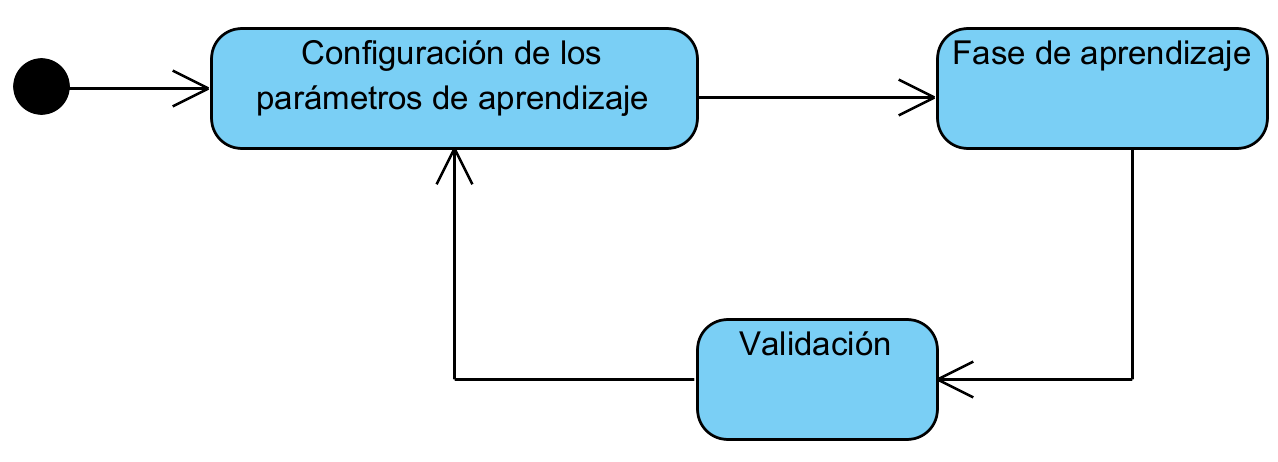
\includegraphics[width=0.7\textwidth]{images/4/Fases.png}
    \caption{Bucle de fases de aprendizaje en un sistema de \texttt{Machine Learning}}
    \label{fig:FasesAprendizaje}
\end{figure}

Dentro del campo existen diferentes ramas dependientes del objetivo del aprendizaje que se busca y los datos con los que vamos a alimentar el sistema:

\begin{itemize}
    \item \textbf{Entrenamiento supervisado}: es un tipo de entrenamiento en el que se conoce la relación entre los datos de entrada y los datos esperados. 
    \item \textbf{Entrenamiento no supervisado}: el objetivo de este aprendizaje es aprender las relaciones de los datos de entrada entre sí.
    \item \textbf{Entrenamiento reforzado}: es una variación del entrenamiento supervisado en el que el sistema recibe feedback sobre los resultados como parte de la fase de aprendizaje. Se utiliza 
    mucho en el ámbito de la robótica.
\end{itemize}

Entre todas las técnicas que implementan este tipo de tareas, uno de los sistemas modernos más conocidos son las redes neuronales.

\subsubsection{Redes Neuronales}

Este campo tiene su origen en una publicación de Warren McCulloch y Walter Pitts en 1943\cite{mccullochLOGICALCALCULUSIDEAS} en el que presentaban la idea de neurona como una unidad lógica básica 
implementable cuyo estado se puede definir como un "todo o nada", lo cual se representa en el campo de las telecomunicaciones con una función escalón como se ve en la \autoref{fig:Escalon}. Este 
trabajo y diseño de neurona sería conocido más tarde como perceptron.

\begin{figure}[H]
    \centering
    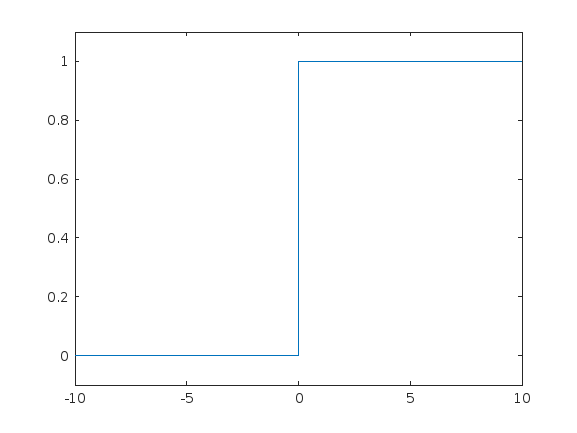
\includegraphics[width=0.3\textwidth]{images/4/Escalon.png}
    \caption{Figura de activación escalón de las primeras neuronas}
    \label{fig:Escalon}
\end{figure}

La estructura básica del perceptron se puede observar en la \autoref{fig:Perceptron} y consiste en un nodo con un número \(\mathcal{N}\) de conexiones entrantes, con un peso asociado \(\mathcal{W}\) 
a cada entrada. El nodo calcula el sumatorio de cada conexión con su respectivo peso. Al resultado de este cálculo se le añade un factor de \texttt{bias} y por último, mediante una función de 
activación como la vista anteriormente, se decide el resultado de salida de la neurona. 

\begin{figure}[H]
    \centering
    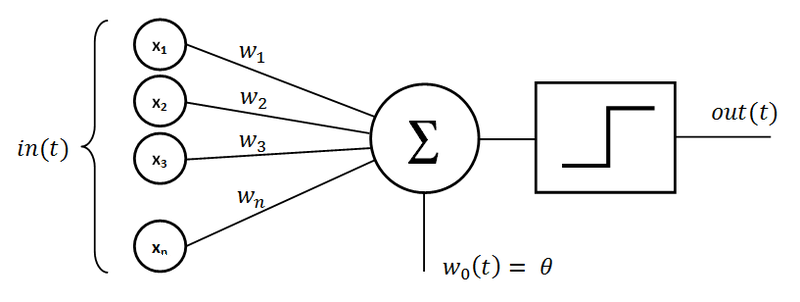
\includegraphics[width=0.5\textwidth]{images/4/perceptron.png}
    \caption{Diagrama general de un perceptron\cite{JgfisherPerceptronPerceptron}}
    \label{fig:Perceptron}
\end{figure}

Más tarde, se conseguiría implementar un diseño electrónico de esta neurona, e interconectar más neuronas entre sí. Estas interconexiones dan lugar a la creación del concepto de \textbf{redes neuronales}, 
siendo una de las primeras redes complejas funcionales de tipo \texttt{\acrfullr{mlp}}. Estos sistemas serían clave para la evolución del aprendizaje automático, apareciendo multitud de 
variaciones en la arquitectura de la red según las necesidades (ver \autoref{fig:ArquitecturasRedes}).

\begin{figure}[H]
    \centering
    \begin{subfigure}[b]{0.25\textwidth}
        \centering
        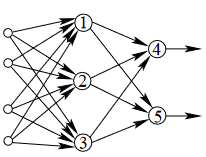
\includegraphics[width=0.9\textwidth]{images/4/FeedForward.png}
        \caption{Red FeedForward}
        \label{fig:a}
    \end{subfigure}
    \begin{subfigure}[b]{0.25\textwidth}
        \centering
        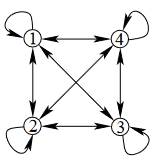
\includegraphics[width=0.7\textwidth]{images/4/Recursiva.png}
        \caption{Red recursiva}
        \label{fig:b}
    \end{subfigure}
    \begin{subfigure}[b]{0.45\textwidth}
        \centering
        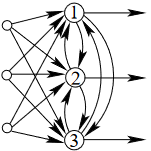
\includegraphics[width=0.4\textwidth]{images/4/FeedForwardLateral.png}
        \caption{Red FeedForward con inhibidores laterales}
        \label{fig:c}
    \end{subfigure}
    \caption{Diferentes ejemplos de arquitecturas simples de redes neuronales\cite{duNeuralNetworksStatistical2013}}
    \label{fig:ArquitecturasRedes}
\end{figure}

El avance progresivo de la capacidad de cómputo de los ordenadores ha permitido el uso de redes neuronales de mayor tamaño, que permiten mayor capacidad de abstracción. Es en este marco donde aparece el término 
\texttt{Deep Learning}, que no indica nada más que el uso de redes neuronales con una cantidad masiva de capas intermedias. Además, son sistemas que trabajan muy bien cuando se implementan con ejecución paralela, 
aunque esto se explicará más adelante.

Este tipo de sistemas han demostrado su gran capacidad de abstracción y rapidez, es por esto mismo que las redes neuronales profundas son una de las principales herramientas que se utilizan hoy en día en 
visión por ordenador.

\clearpage
\subsection{Detección de Objetos con redes neuronales}

La detección de objetos como tarea surge de la necesidad de analizar la existencia de objetos en imágenes y; opcionalmente, localizarlos en las mismas. Para realizar este tipo de tareas se han ido 
desarrollando técnicas tradicionales basadas en algoritmos deterministas, pero, con el auge del aprendizaje automático, a partir de 2012\cite{zouObjectDetection202023} 
el paradigma pasó a centrarse en la creación de sistemas detectores basados en \texttt{Deep Learning} (Sistemas de Redes Neuronales con una gran cantidad de capas ocultas).

Ambas técnicas se basan en la extracción y el análisis de características de las imágenes, esto es, la caracterización de imágenes o zonas de interés a través de algoritmos o filtros. Podemos entender la caracterización 
de una imagen como la parametrización de los elementos que la definen. Dentro de la vista humana existen muchos elementos que se pueden usar para definir una imagen, algunos ejemplos son:
\begin{itemize}
    \item \textbf{Nitidez}.
    \item \textbf{Color}.
    \item \textbf{Presencia de ciertas formas geométricas}.
    \item \textbf{Brillo}.
    \item \textbf{Ruido}
\end{itemize}

Se debe tener en cuenta que estos ejemplos son características que da un humano para una imagen, de forma contraria, las redes neuronales trabajan con características de bajo nivel (P. ej.: existencia de bordes en una zona específica, colores en un área, 
patrones de puntos, etc.) que permitan analizar zonas de la imagen. Sin embargo, las redes neuronales tipo \texttt{\acrshort{mlp}} no fueron pensadas para este tipo de tareas. Esto es debido a que el 
análisis de características en una imagen es una tarea cuya dificultad computacional aumenta de forma exponencial con el aumento de la resolución, ya que, para cualquier imagen, debería haber una neurona de entrada por 
cada pixel y canal de la imagen, sobre cuyos valores la red \texttt{\acrshort{mlp}} aplicaría los cálculos.

Por estos motivos, se buscó una forma de añadir independencia espacial a la entrada de las redes neuronales. Esto se consigue mediante el uso de diferentes arquitecturas, siendo la más importante las redes 
neuronales convolucionales.\newline

\subsubsection{Arquitecturas de redes neuronales tipo \texttt{CNN}}

Las \texttt{\acrfullr{cnn}} definen una arquitectura basada en dos pasos: la extracción de las características de las imágenes y la clasificación de las imágenes según las características. Su estructura básica se 
puede ver \autoref{fig:ArquitecturaCNN} y  se compone de dos subredes que cumplen las dos funciones diferentes para los datos de entrada.

\begin{figure}[H]
    \centering
    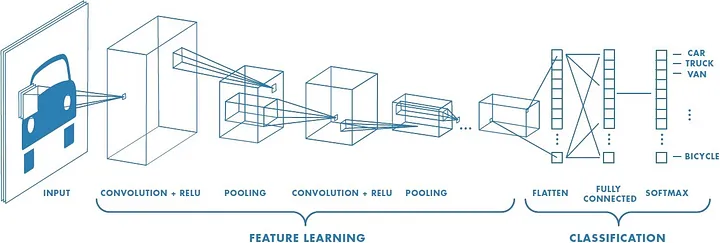
\includegraphics[width=0.9\textwidth]{images/4/ArquitecturaCNN.png}
    \caption{Arquitectura básica de una \texttt{CNN}\cite{sahaComprehensiveGuideConvolutional2022}}
    \label{fig:ArquitecturaCNN}
\end{figure}

\clearpage

La fase de caracterización se compone principalmente de capas neuronales convolucionales y, habitualmente capas de \texttt{pooling}:

\begin{itemize}
    \item Capas convolucionales: tienen como objetivo la extracción de características a través de neuronas que implementan operaciones de convolución sobre las imágenes. 
    Al ser las imágenes tensores, se les aplican filtros convolucionales implementados a través de \texttt{Kernels}. 
    Dependiendo de la característica a buscar, existen diferentes filtros convolucionales y en las fases de entrenamiento se va conformando el \texttt{Kernel} que caracteriza mejor esa zona de la imagen para los datos esperados.

    Un ejemplo de \texttt{Kernel} es un filtro laplaciano gaussiano como el de la \autoref{fig:LaplaceKernel}, que, a través del gradiente, sirve para darle más énfasis a los bordes de la imagen, como se puede ver 
    en la \autoref{fig:LaplaceResultado}.
    \begin{figure}[H]
        \centering
        \(
        \begin{vmatrix}
            1 & 1 & 1 \\
            1 & -8 & 1 \\
            1 & 1 & 1
        \end{vmatrix}
        \)
        \caption{Aspecto de un \texttt{kernel} de Laplace de tamaño \texttt{3x3}}
        \label{fig:LaplaceKernel}
    \end{figure}
    \begin{figure}[H]
        \centering
        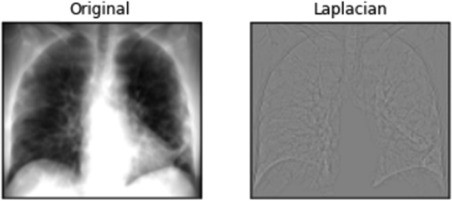
\includegraphics[width=0.7\textwidth]{images/4/KernelsTipicos.jpg}
        \caption{Aplicación de un filtro gaussiano de Laplace a una imagen médica\cite{LaplacianFilterOverview}}
        \label{fig:LaplaceResultado}
    \end{figure}

    Estas capas convolucionales van obteniendo la abstracción de las características transformando los volúmenes de entrada a volúmenes de salida de mayor profundidad pero de menor resolución vertical y horizontal.\newline
    Habitualmente en la parte convolucional se utilizan funciones de activación como la \acrfullr{relu} de la \autoref{fig:relu}.
    \begin{figure}[H]
        \centering
        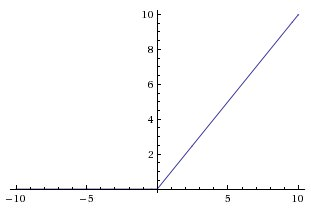
\includegraphics[width=0.5\textwidth]{images/4/relu.jpeg}
        \caption{Función de activación \texttt{ReLU}}
        \label{fig:relu}
    \end{figure}
    \clearpage
    \item Capas de \texttt{pooling}: Su objetivo es ir haciendo sub-muestreo de las capas convolucionales superiores para conformar el volumen de entrada de la siguiente capa convolucional, reduciendo la carga computacional necesaria. 
    Se puede ver su funcionamiento en la \autoref{fig:MuestreoCNN}, donde sub-muestrean un volumen de resolución \texttt{28x28} a una resolución \texttt{14x14}, pero habitualmente se aumenta la profundidad del tensor.
    \begin{figure}[H]
        \centering
        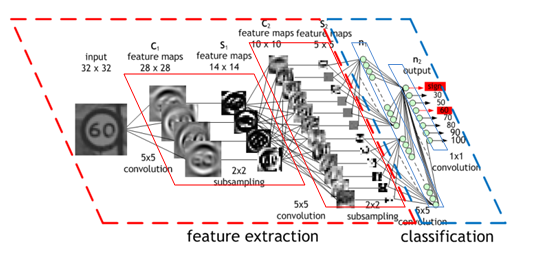
\includegraphics[width=0.6\textwidth]{images/4/EjemploPolling.png}
        \caption{\texttt{CNN} con detalle de la caracterización y el sub-muestreo\cite{ConvolutionalNeuralNetwork}}
        \label{fig:MuestreoCNN}
    \end{figure}
    
    Este sistema se va repitiendo para cada capa de convolución, hasta que en la última capa de \texttt{pooling}, la salida es un vector horizontal cuyo tamaño es el miso que neuronas de entrada tenga la etapa de clasificación. 

\end{itemize}


La fase de clasificación habitualmente se compone de una capa conectada completamente como se ha podido ver en la anterior sección, similar a la idea de una \texttt{\acrshort{mlp}}. Esta 
red toma como entrada un vector aplanado final de la parte de extracción de características y realiza la clasificación. Habitualmente utiliza funciones de activación que son capaces de tener \(\mathcal{N}\) salidas 
una de estas funciones habituales es la \texttt{SoftMax} de la \autoref{fig:softmax}, que mapea un vector de entrada a un vector de salida de probabilidades que escalan según los valores de entrada.

\begin{figure}[H]
    \centering
    \begin{equation*}
        \text{softmax}(z_i) = \frac{e^{z_i}}{\sum_j e^{z_j}}
    \end{equation*}
    \caption{Función de activación \texttt{SoftMax}}
    \label{fig:softmax}
\end{figure}

\vspace{3\baselineskip}

El uso de estas redes neuronales convolucionales para solucionar un problema está asociado al tipo de trabajo a realizar. Cuando se define un problema en el que se va a aplicar esta técnica, normalmente 
cae en tres tipos de categorías presentadas en la \autoref{fig:tareasCNN}. Además, esta selección tiene unas implicaciones en la complejidad computacional de la tarea, ya que la capa de clasificación debe ser cambiada para soportarla.

\begin{itemize}
    \item Clasificación: las imágenes son marcadas dependiendo de si existe o no un elemento específico dentro de ella.
    \item Detección de objetos: regiones locales de la imagen son clasificadas y marcadas dependiendo de la existencia del elemento en cuestión.
    \item Segmentación semántica: se realiza una clasificación por cada pixel para delimitar todos los píxeles que conforman la instancia del objeto.
\end{itemize}

\begin{figure}[H]
    \centering
    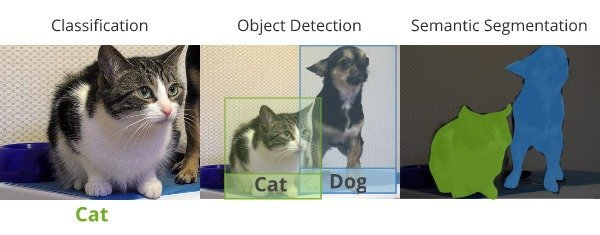
\includegraphics[width=0.6\textwidth]{images/4/TiposTareas.png}
    \caption{Tareas típicas de una \texttt{CNN}\cite{kallfelzsirmacekSEQUENTIALIMAGEPROCESSING2019}}
    \label{fig:tareasCNN}
\end{figure}

Toda red neuronal sobre la que se realice entrenamiento supervisado debe ser entrenada con un conjunto de datos etiquetados de forma coherente a la tarea que se quiera realizar. Por ejemplo, una \texttt{CNN} 
entrenada para clasificar imágenes deberá ser alimentada con etiquetas adecuadas, no con coordenadas sobre la posición del elemento detectado.

Estos conjuntos de datos que se preparan para las redes neuronales se dividen habitualmente en conjuntos con diferentes propósitos en el entrenamiento de la red neuronal:

\begin{itemize}
    \item Conjunto de datos de entrenamiento: es el conjunto de datos sobre el que la red va a aprender, aplicando de forma constante su algoritmo. Pasar por este conjunto entero una vez suele llamarse época 
    de entrenamiento.
    \item Conjunto de datos de prueba: es un conjunto de datos completamente separado que nunca se aplicará a la red en la fase de entrenamiento. Su objetivo es evaluar al final del entrenamiento el 
    rendimiento general de la red en un conjunto de datos que nunca haya visto.
    \item Conjunto de datos de validación: estos datos se utilizan como conjunto de referencia entre épocas, su existencia y uso depende de la arquitectura de red neuronal, ya que existen 
    algunos algoritmos que modifican parámetros del entrenamiento de la red entre épocas.\newline
    Cuando se habla de los parámetros de la red, habitualmente se refieren a cosas como los pesos entre neuronas, la función de activación, el número de capas ocultas, etc\dots Sin embargo, los parámetros 
    que se definen para el entrenamiento como el número de épocas, parámetros del algoritmo de aprendizaje, tamaño de los datos introducidos a la vez, etc., son llamados hiperparámetros.
\end{itemize}

Normalmente se dispone de un conjunto de datos que se divide en entrenamiento, validación y prueba. Es habitual una separación de \texttt{70\%} para el conjunto de entrenamiento, \texttt{15\%} para el conjunto de 
validación y \texttt{15\%} para el conjunto de prueba.

La incorrecta preparación del conjunto de datos puede afectar severamente a los resultados obtenidos. Por lo tanto es habitual intentar evitar redundancia de datos y alimentar a la red con datos que no sean muy 
similares entre sí para que sea capaz de generalizar correctamente en la mayor cantidad de situaciones posibles.\newline
Justo con este propósito podemos encontrar técnicas de aumento de datos, que generan artificialmente datos extra haciendo transformaciones en las imágenes, cambiando el color o incluso aplicando distorsión. 
Esto permite solucionar situaciones en las que se dispongan de pocos datos o los datos sean demasiado parecidos entre sí como para poder asegurar una buena generalización a otros tipos de situaciones.

\clearpage

La evolución de estas \texttt{\acrshort{cnn}} ha sido exponencial y han aparecido arquitecturas que han ido añadiendo mejoras de eficiencia, calidad de resultados y estándares a la hora de crear nuevos 
sistemas. Algunos ejemplos de esto son:
\begin{itemize}
    \item \texttt{R-CNN (Region-CNN)}(2014): introdujo el análisis solo en regiones con datos interesantes.
    \item \texttt{Fast R-CNN} (2015): mejora R-CNN introduciendo búsqueda selectiva, definiendo un número máximo de \texttt{\acrfullr{roi}} a tratar.
    \item \texttt{Faster R-CNN} (2015).
    \item \texttt{\acrfullr{yolo}}\cite{redmonYouOnlyLook2016}: arquitectura extremadamente rápida perteneciente al estado del arte moderno en redes neuronales, que ha ido mejorándose en forma de versiones.
\end{itemize}

Cada arquitectura ha traído consigo mejoras, a veces, a cambio de perdida de rendimiento. Esto es un problema que debe tenerse en cuenta y existen diversos trabajos que tratan simplemente las diferencias 
existentes entre diferentes arquitecturas.

Uno de estos trabajos\cite{hanAdvancedDeepLearningTechniques2018} compara diferentes arquitecturas contra el conjunto de datos de la universidad de Oxford "Pascal2012"\cite{PASCALVisualObject}, que contiene 20 clases de objetos.\newline
Como resultado de este análisis; resumido en la \autoref{ResumenCNN}, se puede observar que \texttt{YOLOv2}, aún no teniendo la mejor precisión, tiene un rendimiento bastante competente. Si nos quedásemos con solo este dato, podríamos llegar a pensar que \texttt{YOLO} 
no tiene por qué ser la mejor elección, pero hay que tener en cuenta el factor de rendimiento, que se mide principalmente en el tiempo que se tarda en realizar la inferencia en una imagen. En este caso, podemos observar 
que \texttt{YOLOv2} es capaz de superar a \texttt{SSD512} obteniendo un mejor \texttt{\acrfullr{map}}(parámetro de caracterización del error medio típico sobre todo el conjunto de datos) con el doble de rendimiento.

\begin{table}[H]
    \begin{center} {\footnotesize
    \begin{tabular}{lcccc}
    \hline
     & \multicolumn{1}{c}{bike} & \multicolumn{1}{c}{bird} & \multicolumn{1}{c}{train} & \multicolumn{1}{c}{mAP}\\
    \hline
    \raisebox{0ex}{Faster R-CNN} & 81.6 & 77.2 & 84.7 & 73.8\\[0ex]
    \raisebox{0ex}{SSD300} & 80.1 & 70.5 & 81.9 & 72.4\\[0ex]
    \raisebox{0ex}{SSD512} & 82.3 & 75.8 & 86.3 & 74.9\\[0ex]
    \raisebox{0ex}{YOLO} & 67.2 & 57.7 & 73.9 & 57.9\\[0ex]
    \raisebox{0ex}{YOLOv2 $544\cdot544$} & 82.0 & 74.8 & 83.8 & 73.4\\[0ex]
    \hline
    \end{tabular} }
    \end{center}
    \caption{Resumen de la comparación entre diferentes arquitecturas de \texttt{CNN} con el conjunto de datos \texttt{PASCAL2012}\cite{hanAdvancedDeepLearningTechniques2018}}
    \label{ResumenCNN}
\end{table}

\begin{table}[H]
    \begin{center} {\footnotesize
    \begin{tabular}{lcc}
    \hline
     & \multicolumn{1}{c}{mAP} & \multicolumn{1}{c}{FPS}\\
    \hline
    \raisebox{0ex}{Faster R-CNN} & 76.4 & 5\\[0ex]
    \raisebox{0ex}{SSD300} & 74.3 & 46\\[0ex]
    \raisebox{0ex}{SSD512} & 76.8 & 19\\[0ex]
    \raisebox{0ex}{YOLO} & 63.4 & 45\\[0ex]
    \raisebox{0ex}{YOLOv2 $544\cdot544$} & 78.6 & 40\\[0ex]
    \hline
    \end{tabular} }
    \end{center}
    \caption{Detalle de rendimiento en \texttt{\acrshort{fps}} en la comparativa de arquitecturas de \texttt{CNN}\cite{hanAdvancedDeepLearningTechniques2018}}
    \label{ResumenCNNFPS}
\end{table}

Estos resultados comparativos, a diferencia de otros artículos\cite{manojkumarPerformanceComparisonReal2023}, son útiles, ya que utilizan reglas tales como la comparación bajo el mismo conjunto de datos e 
indican el tamaño de la imagen de entrada a la red neuronal. Esto permite realizar una comparación realista y en las mismas condiciones.

Podemos observar además, que \texttt{YOLOv2} tiene ciertos problemas al tratar con objetos pequeños. Algunos estudios\cite{bhagyaOverviewDeepLearning2019} ya han observado que es un problema bastante típico de \texttt{YOLO} y es una de las situaciones en las que 
peor funciona.\newline
Estos problemas han ido solucionándose con el tiempo, a través de la mejora y el aumento de rendimiento y puntuación \texttt{\acrshort{map}}. Esto se puede ver en la \autoref{fig:YOLOVersiones}, donde se 
comparan diferentes versiones posteriores a la versión 5 en el conjunto de datos \texttt{COCO}.

\begin{figure}[H]
    \centering
    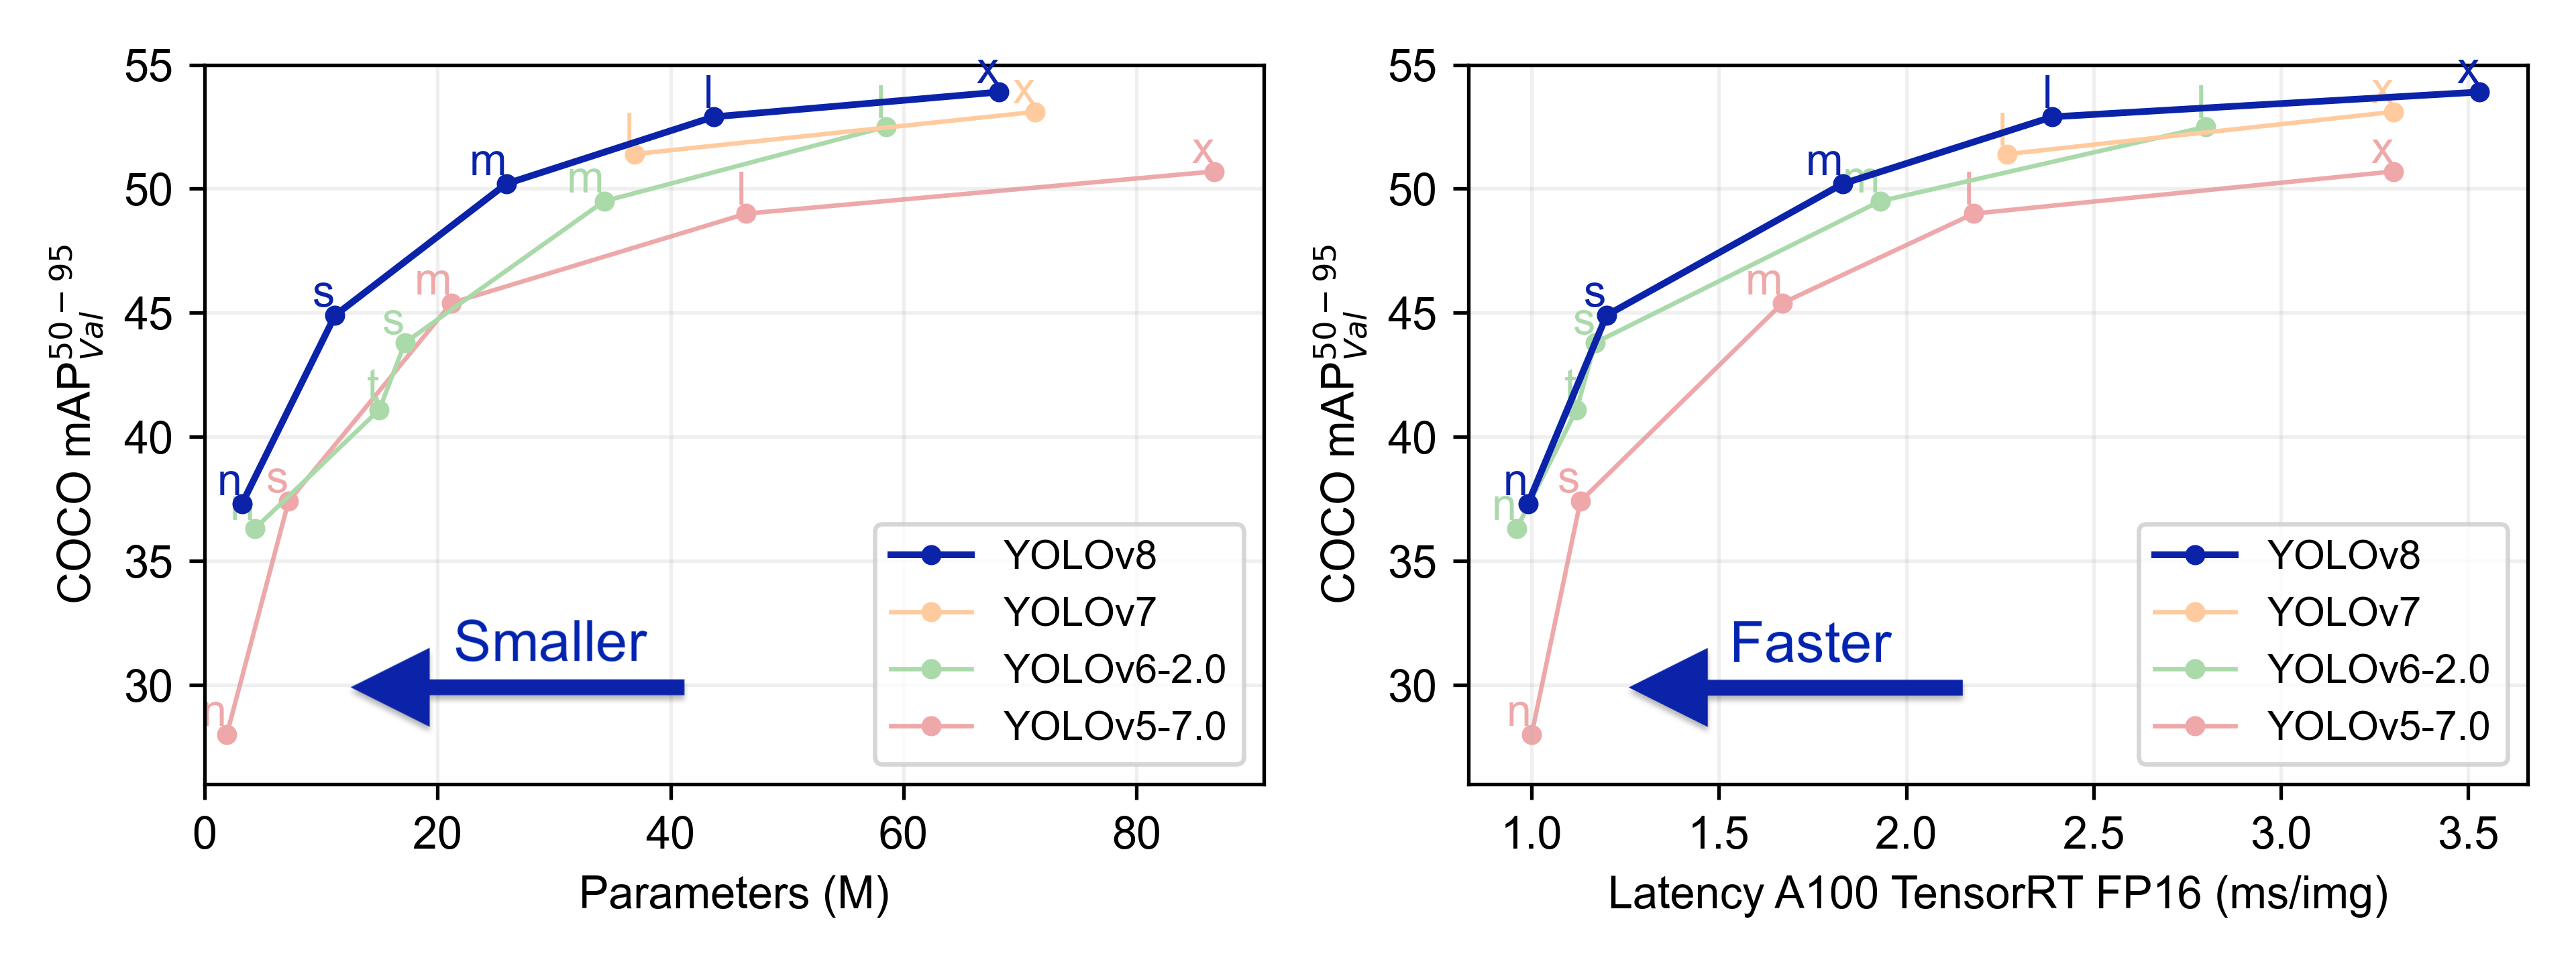
\includegraphics[width=0.8\textwidth]{images/4/YOLOVersiones.png}
    \caption{Rendimiento de diferentes versiones de \texttt{YOLO} superiores a la 5 en el conjunto de datos \texttt{COCO}\cite{ultralyticsYOLOv8}}
    \label{fig:YOLOVersiones}
\end{figure}

Esto ha convertido a \texttt{YOLO} en un estándar de facto en la implementación rápida de soluciones basadas en \texttt{Deep Learning} para muchos investigadores por sus resultados basados en obtener detección en tiempo real.

Actualmente \texttt{YOLO} es un proyecto llevado una la empresa \texttt{ultralytics}, siendo el último modelo \texttt{YOLOv8}. Este modelo está conformado por una capa convolucional personalizada basada en la 
arquitectura \texttt{CSPDarknet53}, basada en conectar diferentes fases de la arquitectura convolucional para obtener un entrenamiento mucho más rápido. Esta capa convolucional se conecta al cuello de \texttt{YOLO}, 
cuya función es utilizar varias salidas de algunas de las secciones de la capa convolucional para tener información de diferentes escalas (cada capa convolucional va transformando la anterior entrada en un vector más y más horizontal).

Lo anterior es común a todos los modelos de \texttt{YOLOv8} independientemente de la tarea que realizan, lo que cambia es la parte final de la red, que, aprovechando la presencia de datos de diferentes escalas, 
utiliza redes neuronales completamente conectadas para diferentes tareas, una para las localizaciones, otra para las probabilidades de clase de cada elemento y otra para trabajar con regiones de interés.

Para facilitar la lectura del documento, en el \hyperref[subsec:A]{anexo A} se realiza una explicación detallada de los parámetros e hiperparámetros habituales de los modelos de \texttt{YOLOv8} y una explicación 
de los estadísticos que parametrizan la calidad de los entrenamientos de la red en los modelos \texttt{YOLOv8}.


\subsubsection{Uso de redes neuronales en acuicultura}

La acuicultura es un trabajo que engloba desde la producción de algas hasta la crianza de marisco en cautiverio. Además, dentro de cada rama podemos tener especies que sean similares y que deban ser diferenciadas.

En la literatura de este ámbito se lleva implementando tecnologías basadas en aprendizaje automático para diferentes tareas, en el caso del uso de \texttt{\acrshort{cnn}} podemos ver sistemas para:
\begin{itemize}
    \item Sistemas de conteo de peces\cite{castillomoralSistemaConteoPeces2022}.
    \item Sistemas de análisis de densidad.
    \item Sistemas de seguimiento\cite{leeDetectionCatfishActivity2024}.
    \item Sistemas de diferenciación y detección de especies en entornos abiertos\cite{xiaSituSeaCucumber2018}\cite{ladeAutomatedFishSpecies2023}: aprovechando la existencia de conjuntos de datos
    \cite{ulucanLargeScaleDatasetFish2020} para experimentos con diferentes peces.
\end{itemize}

Existen ejemplos del uso de estas tecnologías son proyectos como el del \acrfullr{citsem} ``Acuicultura 4.0"\cite{Acuicultura} y diversos trabajos de fin de grado y máster relacionados, pero no para el conteo de movimientos a través de YOLO.

\clearpage
\subsection{Técnicas para el análisis de movimiento en la visión por ordenador}

Estas técnicas son muy importantes en el campo de la vigilancia, para poder percibir el cambio de elementos en la imagen y realizar su seguimiento. Según los autores M.Sonka y V.Hlavac\cite{sonkaImageProcessingAnalysis2013}, los problemas que 
trata se pueden dividir en tres grupos:

\begin{itemize}
    \item Detección de movimiento general, clasificando una imagen con o sin movimiento a través de un descriptor global.
    \item Detección y localización de objetos en movimiento, donde la escena es estática y el objeto se mueve sobre ella.
    \item Uso del movimiento para la reconstrucción 3D de una escena.
\end{itemize}

De los anteriores puntos, el más relevante en este trabajo es la detección y localización de objetos en movimiento (conteo de movimiento de un pez).

Debemos entender que el análisis de movimiento tiene en cuenta el eje temporal entre las imágenes, que puede tener muestras equiespaciadas o no. Es en este eje sobre el que queremos realizar el análisis, pero 
cabe destacar que hay muy poco análisis realizado sobre el uso de aprendizaje automático para estimación de movimiento en video. Los principales sistemas se basan en análisis a través de algoritmos.

\begin{itemize}
    \item \textbf{Análisis diferencial}: un ejemplo de esta técnica es la resta de una imagen número $n$ con la imagen número $n-1$, para obtener una diferencia de en ciertos pixeles y determinar a través de un límite 
    la existencia de movimiento. Uno de los tipos de algoritmos más interesantes en este campo es el análisis de flujo óptico.
    \item \textbf{Correspondencia de puntos de interés}: se basa en la detección y seguimiento a través del eje temporal de ciertos puntos claves, para detectar el movimiento de elementos. Existen operadores para este 
    objetivo, pero no se adaptan bien a cambios demasiado rápidos.
    \item \textbf{Detección de patrones de movimiento}: uno de los pocos sistemas que se basa en entrenar un clasificador capaz de detectar patrones de movimiento, sin embargo son herramientas muy complejas 
    de implementación y tienen un alto coste computacional, ya que normalmente realizan las tres tareas: detección, clasificación y segmentación.
\end{itemize}

La mayoría de herramientas desarrolladas en este campo tienen necesidades muy específicas y no se adaptan bien a cambios demasiado bruscos, la única que puede manejarlos es una herramienta como el análisis de flujo óptico. 
Esto es debido a que se puede usar para analizar cambios entre todos los píxeles de las imágenes.

\subsubsection{Definición y uso del análisis de flujo óptico}

El análisis de flujo óptico u \texttt{OpticalFlow} apareció por primera vez en 1981\cite{hornDeterminingOpticalFlow1981} y se basa en asumir:

\begin{enumerate}
    \item El brillo observado en un punto del objeto es constante en el eje temporal.
    \item Puntos cercanos se mueven de la misma manera.
\end{enumerate}

El problema es que en las imágenes reales las reglas sobre el brillo y la suavidez del cambio es habitual que no sean respetadas. Esto puede ser por diversos motivos como poco \texttt{framerate} o movimientos 
muy cercanos a la cámara que generen cambios bruscos en los pixeles.

Es una técnica que se usa mucho en las carreteras, por la existencia de entornos muy estáticos. Se puede ver un ejemplo de su aplicación en la \autoref{fig:OpticalFlowEjemplo}.

\begin{figure}[H]
    \centering
    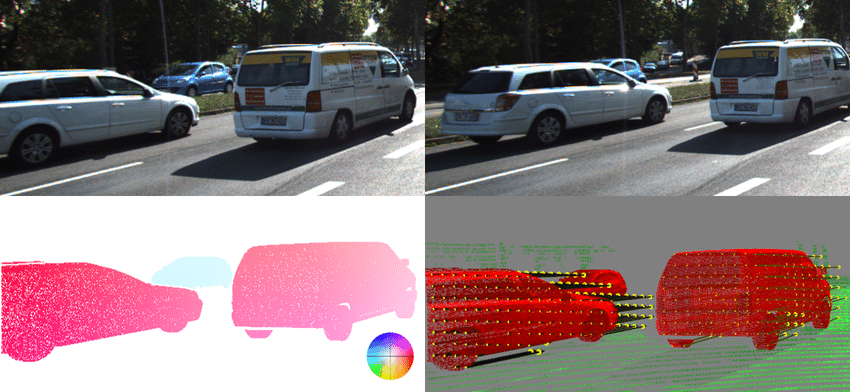
\includegraphics[width=0.8\textwidth]{images/4/OpticalFlow.png}
    \caption{Análisis del flujo óptico entre 2 fotogramas de una escena\cite{schusterCombiningStereoDisparity2018}}
    \label{fig:OpticalFlowEjemplo}
\end{figure}

Actualmente, existen tres algoritmos principales para calcular el flujo óptico de una escena:

\begin{itemize}
    \item Método Horn-Schunck: devuelve una estimación global.
    \item Método de Lucas-Kanade: asume que el flujo va a ser constante en los vecinos, y con esto, realiza una serie de estimaciones locales.
    \item Método combinado local-global: calcula el flujo óptico en zonas rectangulares de la imagen.
\end{itemize}

\subsubsection{Uso del análisis del flujo óptico en entornos de acuicultura}

El análisis de flujo óptico se ha usado en acuicultura de forma diversa:

\begin{itemize}
    \item Analizar comportamientos de grupo, por ejemplo, para determinar la actividad de un conjunto de peces de forma global\cite{kobayashiAquaColonyFully2023}.
    \item Realizar una detección, conteo y seguimiento de peces en un tanque en la India, mezclando \texttt{YOLOv5} con \texttt{OpticalFlow}\cite{paiComputerVisionBased2022}. Este método dio buenos resultados porque 
    la distancia del pez a la cámara era lo suficientemente grande como para que no hubiese movimientos demasiado grandes como se puede ver en la \autoref{fig:DatosOpticalEstudio}.
\end{itemize}

\begin{figure}[H]
    \centering
    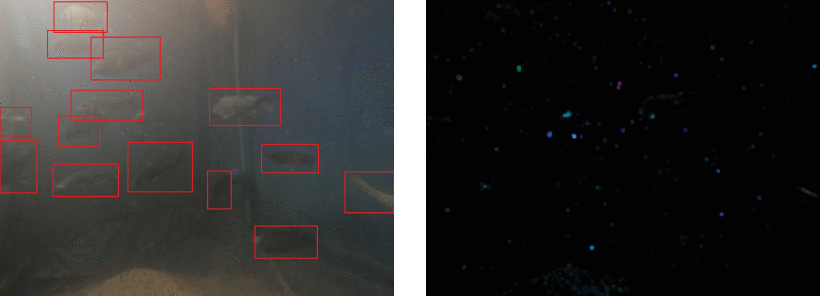
\includegraphics[width=0.9\textwidth]{images/4/OpticalFlowIndia.png}
    \caption{Datos obtenidos por OpticalFlow respetando las reglas de distancia sobre peces\cite{paiComputerVisionBased2022}}
    \label{fig:DatosOpticalEstudio}
\end{figure}
\clearpage


\subsection{Herramientas de desarrollo y despliegue en \texttt{HardWare} transparente}

\begin{itemize}
    \item \textbf{Librerías de desarrollo para Redes Neuronales}: Para trabajar en la creación de redes neuronales, se usan principalmente dos librerías: \texttt{Keras} y \texttt{PyTorch}.
    \texttt{Keras} es una librería de alto nivel, mientras que \texttt{PyTorch} es de bajo nivel y tiene mejores herramientas de manejo de errores y de control del rendimiento de la red creada. 
    Aparte de esto, \texttt{PyTorch} está pensado para su uso directamente en \texttt{Python} y soporta entrenamiento en sistemas distribuidos.


    En el caso de \texttt{YOLO}, la empresa \texttt{Ultralytics} retomó el proyecto y creo las versiones a partir de \texttt{YOLOv5}. El objetivo de esto ha sido crear una librería para 
    que el usuario no tenga que interactuar con las librerías de bajo nivel. Esto nos permite entrenar, validar y desplegar modelos a través de modelos base.
    \item \textbf{Transfer Learning y Fine Tunning}: Entrenar una red neuronal desde 0 es demasiado complejo, por ejemplo, una red \texttt{YOLOv8} de tamaño pequeño tiene \texttt{11.2} millones de pesos que 
    deben ser entrenados y ajustados. Estos pesos son contabilizando las capas convolucionales y la capa de clasificación.\newline
    Pero lo habitual es obtener un modelo ya entrenado, cuyas capas convolucionales sean capaces de extraer características típicas de cualquier imagen y, solo entrenar la parte de clasificación. 
    Esto reduce mucho el coste computacional de entrenamiento y por lo tanto, el tiempo requerido para llegar al objetivo deseado con la red. Esta técnica se conoce como \texttt{Transfer Learning} 
    y se puede ver en la \autoref{fig:TransferLearning}.
    
    \begin{figure}[H]
        \centering
        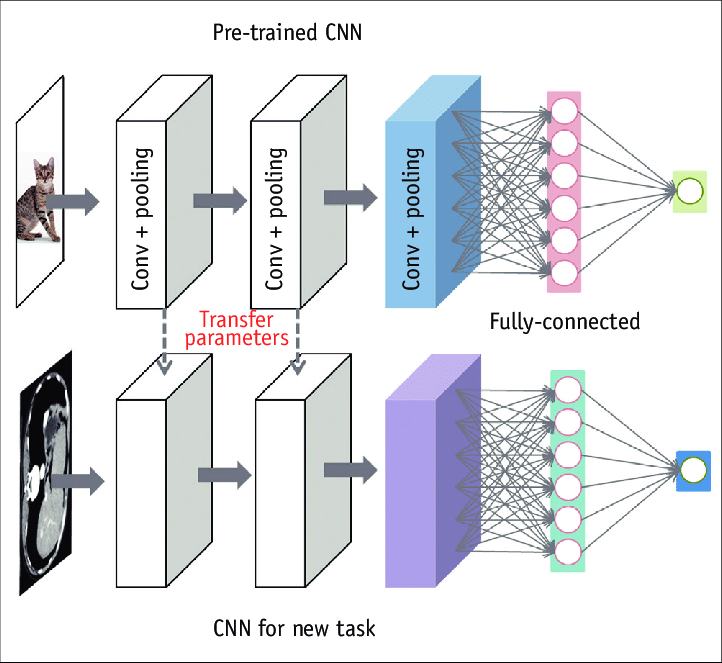
\includegraphics[width=0.65\textwidth]{images/4/TransferLearning.png}
        \caption{Uso de parámetros realizando \texttt{Transfer Learning}\cite{doBasicsDeepLearning2020}}
        \label{fig:TransferLearning}
    \end{figure}

    Posteriormente, cuando se alcanza el rendimiento esperado, se pueden desbloquear los pesos de las capas de convolución y hacer entrenamiento de toda la red. Esta fase se llama \texttt{Fine Tunning}. 
    Su objetivo es ajustar la capa de convolución también para solo analizar las características de la imagen más relevantes para la tarea.
    \item \textbf{Herramientas comunes para el análisis de flujo óptico}: En la mayoría de lenguajes existen librerías que implementan los algoritmos de análisis de flujo óptico, pero, al ser herramientas de 
    caracterización de imagen, existen muchas facilidades en entornos matemáticos como MATLAB o de procesado de datos como el lenguaje de programación \texttt{Python}, más concretamente la librería de \texttt{OpenCV}.
    
    \clearpage
    
    \item \textbf{Abstracción de la red neuronal al \texttt{HardWare}}: A la hora de desplegar una red neuronal, se debe diseñar una estrategia para 
    poder aprovechar todos los recursos del sistema que va a ejecutar la red. Esto es debido a que una red neuronal se aprovecha de la computación en paralelo, ya que principalmente 
    resuelve problemas y multiplicaciones con matrices.

    En este sentido, los despliegues más eficientes son los que son capaces de aprovechar elementos como las \texttt{\acrfullr{gpu}}, que se centran en este tipo de operaciones. Al contrario 
    que una \texttt{\acrfullr{cpu}}, la \texttt{\acrfullr{gpu}} cuenta con más núcleos de cómputo de menor potencia como se puede ver en la \autoref{fig:GPUCPU}.

    \begin{figure}[H]
        \centering
        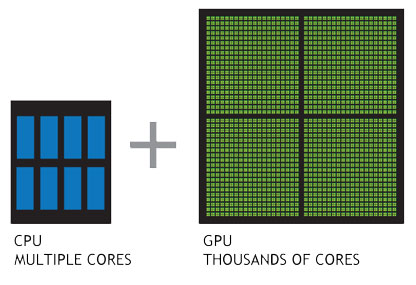
\includegraphics[width=0.5\textwidth]{images/4/GPUCores.jpg}
        \caption{Diferencia de cantidad de núcleos en una \texttt{CPU} y una \texttt{GPU}\cite{GPUVsCPU}}
        \label{fig:GPUCPU}
    \end{figure}

    En este sentido, según la plataforma de desarrollo de red neuronal que se utilice, el despliegue podrá aprovechar la gráfica dependiendo de factores como:
    
    \begin{itemize}
        \item Marca: \texttt{NVidia}, \texttt{AMD} o \texttt{Intel}.
        \item Generación del \texttt{HardWare}.
        \item Sistema Operativo en el que se despliega el sistema.
    \end{itemize}

    Por ejemplo, una red neuronal desarrollada en PyTorch solo soporta gráficas de \texttt{AMD} si el sistema operativo es \texttt{Linux}. Es por este motivo 
    que han surgido librerías abiertas que permiten el uso de una aceleración por \texttt{HardWare} común a muchos más dispositivos. Ejemplo de esto son los modelos 
    desarrollados en el entorno \texttt{ONNX}.
    De hecho, algunas empresas como \texttt{Intel} desarrollan sus propias librerías de herramientas para permitir compatibilidad con sus sistemas de aceleración. Estas librerías 
    suelen contener además, herramientas de transformación entre modelos para aportar más transparencia al usuario final y evitar problemas de compatibilidad.
\end{itemize}

\newpage
\thispagestyle{abstract}
\mbox{}
\newpage
\section{DESCRIPCIÓN DE LA SOLUCIÓN PROPUESTA}
Se busca desarrollar una aplicación completa que sirva como sistema en gran medida automatizado para obtener una estimación 
de los movimientos realizados por truchas en videos de experimentos \textit{NetTest}. Para realizar esta tarea, se diseñará 
una arquitectura dividida en tres sistemas específicos como se puede ver en la \autoref{fig:ArquitecturaBasicaSolucion}.

\begin{itemize}
    \item Interfaz gráfica de usuario: permitirá al usuario seleccionar el video a analizar, observar los resultados y guardarlos.
    \item Capa de análisis del video: a través de técnicas como el \texttt{Machine Learning} o el análisis de flujo óptico, parametrizará 
    los movimientos de las truchas que aparezcan en el video.
    \item Capa de procesado de datos: obtendrá la caracterización realizada por la capa de análisis y a través de la transformación y 
    procesado de los datos, devolverá los datos que se deban mostrar en la interfaz gráfica. Además realizará la estimación final del número 
    de movimientos por trucha.
\end{itemize}
\begin{figure}[H]
    \centering
    \includegraphics[width=\textwidth]{images/6/IdeaAplicación.png}
    \caption{Arquitectura básica de la solución propuesta}
    \label{fig:ArquitecturaBasicaSolucion}
\end{figure}

El bucle de uso principal consistirá en la selección de un video a procesar, el análisis del mismo, la transformación de los datos resultantes, 
la estimación de los movimientos y la devolución de los datos al usuario a través de la interfaz gráfica.\newline
El usuario podrá elegir verificar los datos o guardar directamente un archivo con los resultados. Realizado esto, el usuario podrá volver a la 
pantalla inicial para seleccionar otro video para continuar con el proceso.

La solución se implementará de manera que se puedan aprovechar al máximo los recursos del sistema, permitiendo una reducción en el tiempo global 
que toma procesar un experimento.

En los siguientes puntos, se explicarán los datos con los que se va a trabajar y se detallará los pasos seguidos para el desarrollo de la solución propuesta.

Para explicar la implementación de la propuesta, se empezará por los componentes internos del módulo de obtención de datos, luego se detallaran 
los procesos de transformación de datos y finalmente el desarrollo de la aplicación completa con interfaz.


\clearpage

\section{DESCRIPCIÓN DE LOS DATOS}

Como se ha comentado anteriormente, la búsqueda por mejorar las condiciones animales en los procesos de crianza ha fomentado la investigación en 
diferentes marcadores biológicos relacionados con el estrés.

El \acrfullr{pran}\cite{ObservatorioUPM}, perteneciente a la \acrfullr{ETSIAAB}, realiza investigaciones en estas líneas, siendo una principal el bienestar animal en peces, 
usando experimentos como el \textit{NetTest}.

A partir de estas labores anteriores de investigación, se han podido obtener materiales para este trabajo, siendo principalmente videos del experimento junto a sus etiquetas. Para obtener 
estos datos, en sucesivos trabajos del \acrshort{pran} se ha utilizado la herramienta \textit{BORIS}\cite{friardBORISFreeVersatile2016}, que ha permitido anotar diferentes momentos en los que 
ha sucedido un movimiento.

En concreto, el grabado y etiquetado manual se llevó a cabo por los técnicos Juan Enrique Barrios Sánchez\cite{barriossanchezPruebaRedEvaluando2023}  y Almudena Gallego Fernández, bajo la supervisión de los investigadores 
Álvaro De la LLave-Propín y Morris Villarroel Robinson.

Por lo tanto, el etiquetado manual no siempre se ha llevado a cabo por la misma persona, con lo que puede existir un factor de subjetividad que añade error humano a la medición de los 
movimientos de los peces.

\subsection{Conjunto de datos disponibles: videos}

Los videos se pueden separar en 2 subconjuntos dependiendo del momento en el que se realizó la grabación, lo cual se ve reflejado en la calidad de la misma y la facilidad para identificar el movimiento 
del pez a lo largo de los fotogramas.

\subsubsection{Videos antiguos}

Para este tipo de videos se cuenta en total con un conjunto de 6 videos completos de un experimento \textit{NetTest} sobre todos los peces de un grupo, pero no se tiene más información relevante sobre 
los especímenes que aparecen en los videos.

Se tratan de videos en formato \texttt{16:9}, con resolución \texttt{1920x1080}, con la cámara posicionada fija verticalmente encima de una mesa donde se lleva a cabo el experimento. Esto se puede ver 
en la \autoref{fig:ExperimentoAntiguo}. En este caso, el experimento se lleva a cabo con redes negras, lo cual puede ser problemático teniendo en cuenta que los peces tienen 
tonalidades similares al marrón y gris.

\begin{figure}[h]
    \centering
    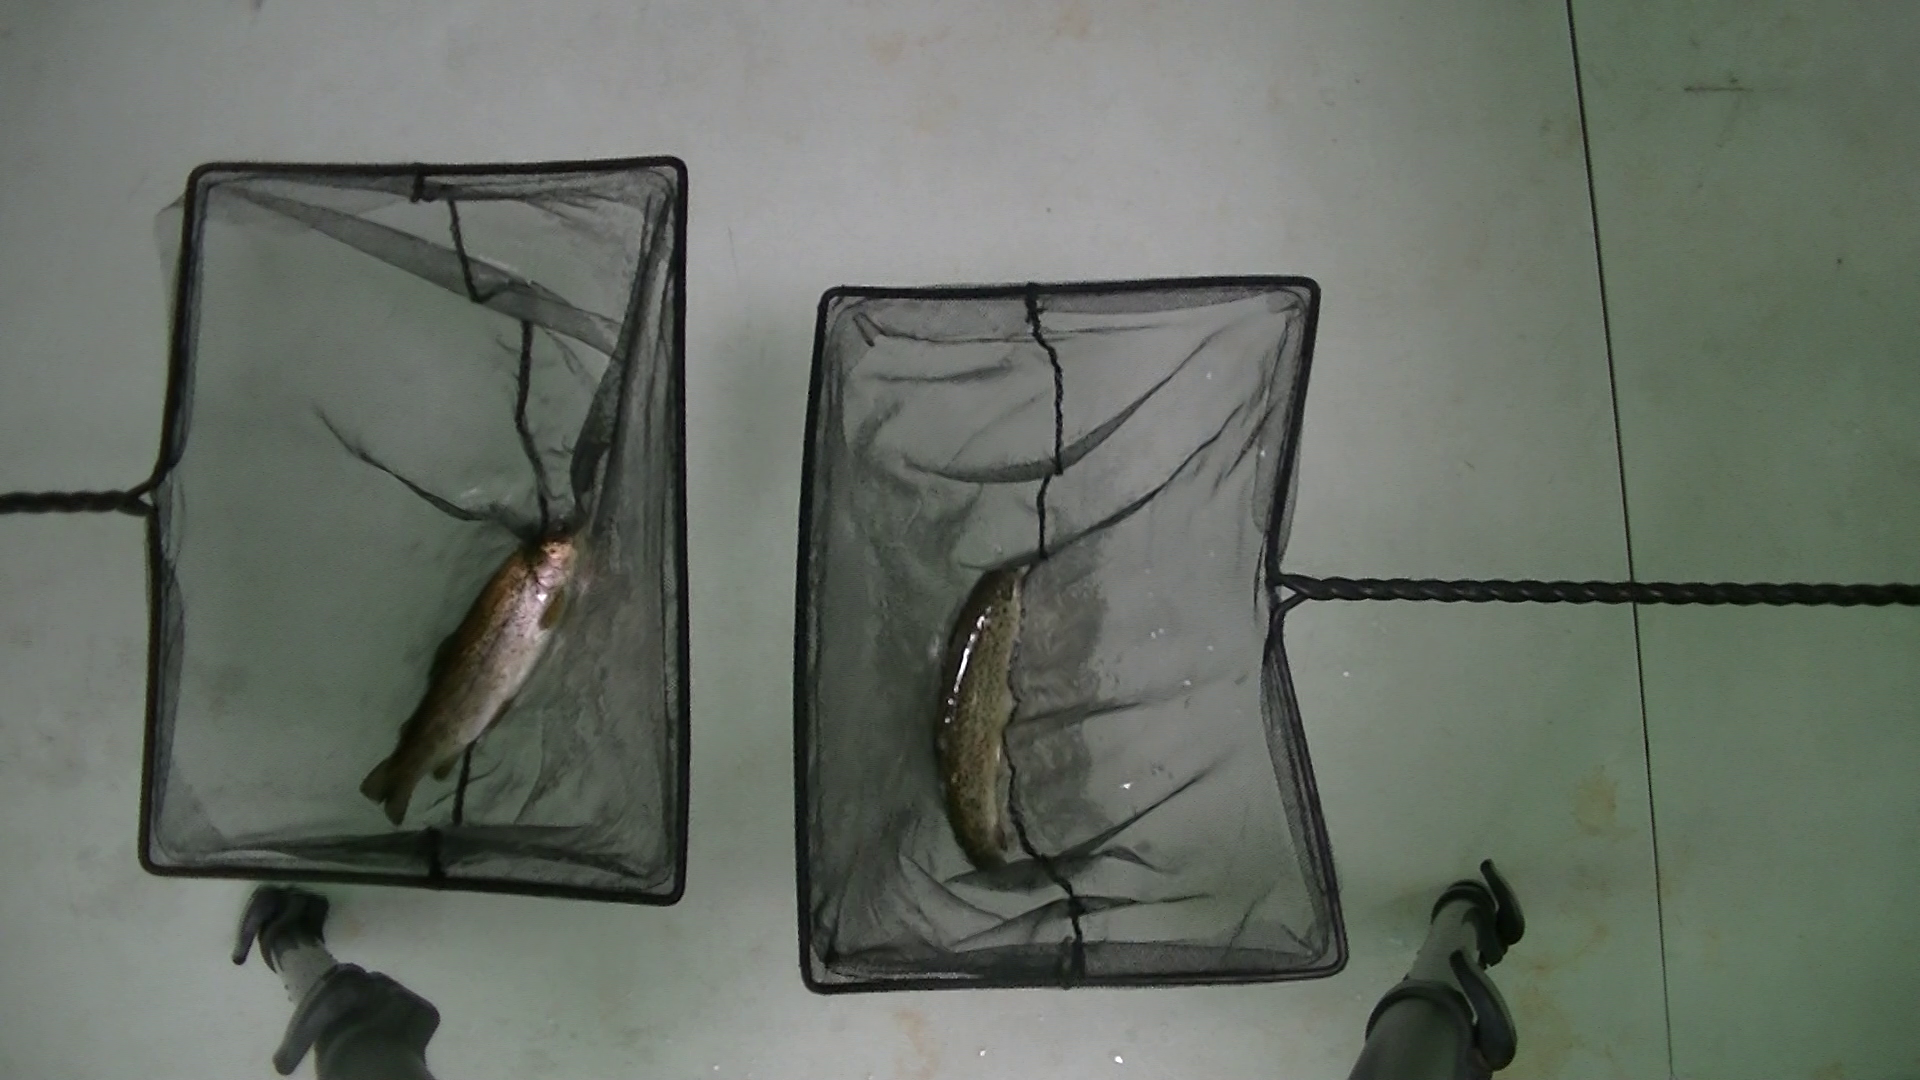
\includegraphics[width=0.70\textwidth]{images/3/ExperimentoAntiguo.png}
    \caption{Aspecto de los videos más antiguos}
    \label{fig:ExperimentoAntiguo}
\end{figure}

Las especificaciones de la cámara en el momento de grabación son desconocidas, pero a través de los detalles de los archivos se observa que son archivos con extensión 
\textit{\acrfullr{mts}}, grabados a 25 \acrshort{fps} y con una tasa de datos por segundo de \texttt{16.96 Mbps}.

En estos videos, se realizan el experimento 5 veces con 2 peces a la vez para maximizar el tiempo. Por lo tanto, puede ser necesario segmentarlo manualmente.

Como último punto importante, en estos videos se puede observar que se realiza la variación del \textit{NetTest} que dura 1 minuto aproximadamente.

\subsubsection{Videos nuevos}

Este es el conjunto de datos más amplio y detallado. Cuenta en total con 4 experimentos \textit{NetTest}, en los que se realiza el experimento a 10 jaulas en total (10 peces por jaula en parejas). 
Cada jaula consta de un  video que muestra el experimento entero y luego una serie de subvideos que los investigadores de \acrshort{pran} han sacado recortando el original para eliminar 
momentos en los que no hay ningún experimento en pantalla. Esta estructura final se puede ver en la \autoref{fig:EstrucutraNuevos}.

\begin{figure}[h]
    \centering
    \begin{subfigure}[b]{0.5\textwidth}
    \dirtree{%
    .1 \vdots.
    .1 \textbf{Net Test 1}.
    .2 \vdots.
    .1 \textbf{Net Test 2}.
    .2 \vdots.
    .2 \textbf{Jaula 7}.
    .3 \textbf{23 NT R2 J7}.
    .3 \textbf{23 NT R2 J7 P1-2}.
    .3 \vdots.
    .3 \textbf{23 NT R2 J7 P9-10}.
    .2 \vdots.
    .1 \textbf{Net Test 3}.
    .2 \vdots.
    .1 \textbf{Net Test 4}.
    .2 \vdots.
    }
    \end{subfigure}
    \caption{Estructura de los  videos nuevos}
    \label{fig:EstrucutraNuevos}
\end{figure}

Hay que tener en cuenta que para los videos siempre se sigue el orden \textit{\acrfullr{ltr}}. Por ejemplo, para el video \verb|23_NT_R2_J2_P1_2|, el pez de la izquierda será el pez número 1 y 
el pez de la derecha el número 2.

Los videos mantienen las características de formato en \texttt{16:9}, con resolución \texttt{1920x1080} y cámara apuntando verticalmente a la mesa del experimento 
(\autoref{fig:ExperimentoNuevo}), sin embargo, podemos ver que se ha pasado a usar una red verde que aporta cierto contraste respecto al cuerpo del pez. Aparte de esto, 
el marco de la red también ha cambiado y tiene un color plateado. En otros experimentos como los del \textit{NetTest}3 también se observa el uso de redes negras.

\begin{figure}[H]
    \centering
    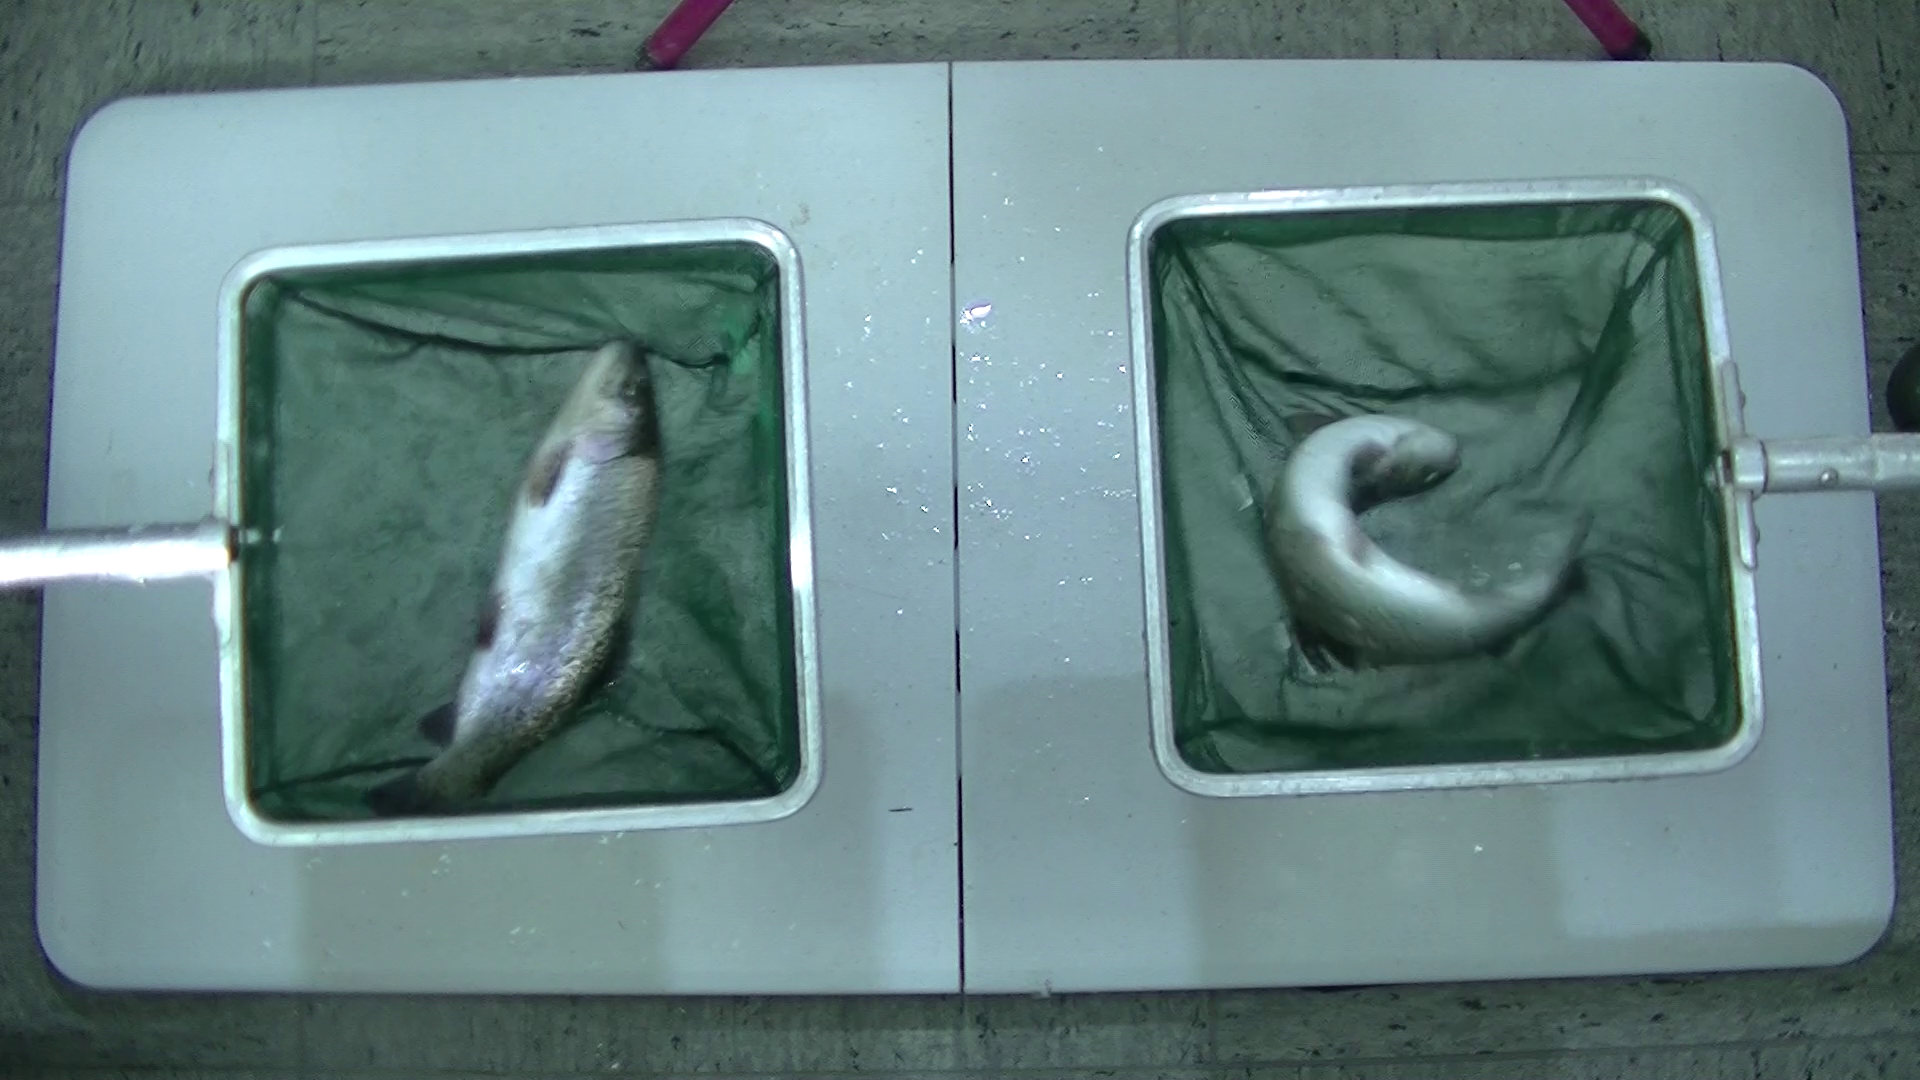
\includegraphics[width=0.7\textwidth]{images/3/ExperimentoNuevo.png}
    \caption{Aspecto de los videos nuevos}
    \label{fig:ExperimentoNuevo}
\end{figure}

Las especificaciones de la cámara para estos videos siguen siendo desconocidas, pero se puede asumir que los parámetros han cambiado por el aumento de la luminosidad de la imagen.
Además, se ha movido un poco la colocación de la mesa y la línea negra queda justo en el medio entre las dos truchas con las que se realiza el experimento.

Respecto a datos técnicos del video, el contenedor ha cambiado a \textit{\acrfullr{mov}}, se mantienen los 25 \acrshort{fps} y la tasa de datos aumenta hasta los \texttt{21 Mbps}.

Los videos obtenidos en este caso también contienen videos de experimentos en grupo, es decir, varios experimentos a varias parejas de truchas. Sin embargo, a diferencia de los videos antiguos, 
en este caso los experimentos \textit{NetTest} duran 15 segundos aproximadamente.

\subsection{Conjunto de datos disponibles: etiquetas}

Por motivos ajenos a este trabajo, no se cuentan con las etiquetas manuales correspondientes a los videos antiguos. Esto implica que no se tiene un marco de referencia para 
contar los movimientos de los videos más antiguos.

\subsubsection{Videos nuevos}

Existen dos archivos \texttt{Excel}, el primero de ellos contiene toda la información sobre los experimentos:
\begin{itemize}
    \item Chip de cada individuo del experimento por grupo, pez y \textit{NetTest}.
    \item Pez de cada grupo y \textit{NetTest}.
    \item Todos los fotogramas en los que cada pez ha realizado un movimiento, tomando como referencia el fotograma 0 del video no recortado.
    \item Momento en el tiempo del video en el que sucede cada movimiento, tomando como referencia el tiempo del video no recortado.
\end{itemize}

De todos los datos, los útiles van a ser los referentes a los movimientos, que se pueden ver en la \autoref{fig:Excel1}. Esto se debe a que los datos sobre el chip no nos aportan información.

\begin{figure}[H]
    \centering
    \fbox{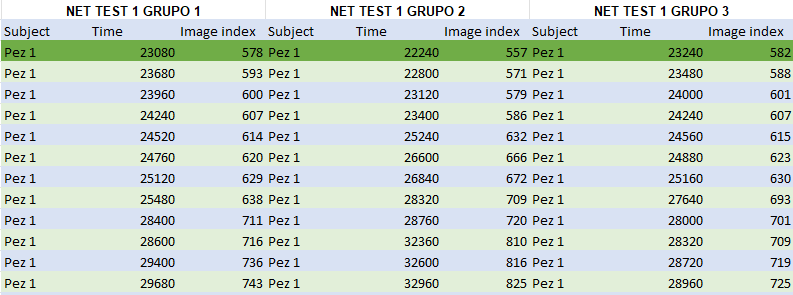
\includegraphics[width=0.7\textwidth]{images/3/Excel1.png}}
    \caption{Columnas del \texttt{Excel} con los datos de los fotogramas en los que sucede un movimiento}
    \label{fig:Excel1}
\end{figure}
El segundo archivo \texttt{Excel} nos proporciona información ya procesada por los investigadores del \acrshort{pran}, en los cuales aparecen 
los movimientos finales totales para cada pez según grupo y número de experimento \textit{NetTest}. Un ejemplo de una sección del archivo se 
puede ver en la \autoref{fig:Excel2}.

\begin{figure}[H]
    \centering
    \fbox{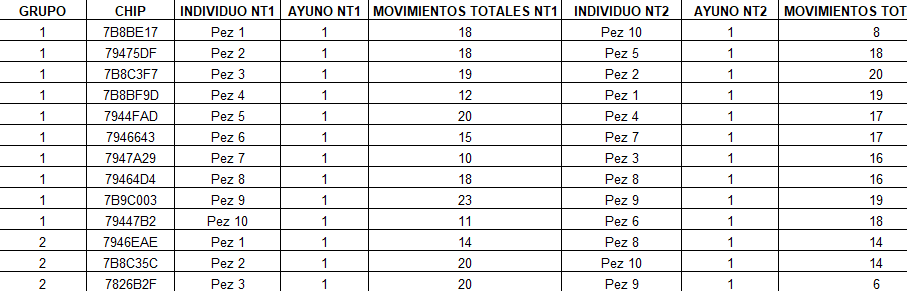
\includegraphics[width=0.7\textwidth]{images/3/Excel2.png}}
    \caption{Sección del archivo de movimientos finales para los videos nuevos}
    \label{fig:Excel2}
\end{figure}


\newpage
\thispagestyle{abstract}
\mbox{}
\newpage
\section{REQUISITOS Y RESTRICCIONES DE DISEÑO}

Como proyecto de ingeniería, el análisis previo de requisitos y restricciones del sistema se ha realizado para modelar el comportamiento esperado 
resultante del desarrollo de la solución propuesta

Dentro del análisis de requisitos, se han diferenciado entre funcionales(definiciones del comportamiento del sistema) y no funcionales(definiciones de atributos de control de calidad).

\subsection{Análisis de requisitos}
\begin{table}[H]
    \begin{center}
        \begin{tabular}{p{0.1\textwidth} | p{0.7\textwidth} p{0.1\textwidth}}
            Req. ID & Descripción de requisito funcional & Prioridad\\
            \hline
            0& Los cálculos automáticos deben ser transparentes a los conocimientos del usuario & Alta\\
            \hline
            1& El usuario deberá poder seleccionar el nivel de agresividad del sistema & Media\\
            \hline
            2& Se deberá llevar un registro por usuario de las predicciones anteriores & Baja\\
            \hline
            3& El usuario debe poder cambiar de usuario & Baja\\
            \hline
            3& El usuario debe poder ver cuáles usuarios existen & Baja\\
            \hline
            4& La inferencia debe hacerse posterior a la selección y confirmación del video & Alta\\
            \hline
            5& El usuario deberá poder seleccionar diferentes formatos de video sobre los que inferir de forma transparente & Alta\\
            \hline
            6& Si ocurre un error en la selección de fichero, se informará por un pop-up & Alta\\
            \hline
            7& La inferencia se realizará de forma transparente al usuario en una pantalla de carga & Alta\\
            \hline
            8& La inferencia se podrá cancelar para evitar perdidas de tiempo & Media\\
            \hline
            9& En la pantalla de carga se informará de cuanto queda para acabar la inferencia & Alta\\
            \hline
            10& Si ocurre un error en la inferencia se deberá informar con un pop-up y volver a la pantalla inicial & Alta\\
            \hline
            11& Se deberá hacer la inferencia en paralelo para no colgar la aplicación & Alta\\
            \hline
            12& Si se completa la inferencia, deberá pasarse a la pantalla de resultados & Alta\\
            \hline
            13& En la pantalla de resultados el usuario deberá poder elegir guardarlos en csv y excel & Alta\\
            \hline
            14& En la pantalla de resultados el usuario debe poder verificar los resultados obtenidos & Alta\\
            \hline
            15& En la pantalla de resultados el usuario debe poder añadir o eliminar movimientos de los resultados obtenidos & Media\\
            \hline
            16& En la pantalla de resultados el usuario debe poder volver a la pantalla inicial & Media\\
            \hline
            17& En la pantalla de resultados el usuario puede elegir guardar estos resultados en su perfil (sin guardar el video, solo el registro de movimientos y el nombre del video) & Bajo\\
            \hline
            18& Si el usuario guarda un resultado por primera vez, ese nuevo usuario se quedará registrado en la aplicación  & Bajo\\
            \hline
        \end{tabular} 
    \end{center}
    \caption{Análisis de requisitos funcionales}
    \label{ReqFuncionales}
\end{table}

\begin{table}[H]
    \begin{center}
        \begin{tabular}{p{0.1\textwidth} | p{0.7\textwidth} p{0.1\textwidth}}
            Req. ID & Descripción de requisito no funcional & Prioridad\\
            \hline
            0& Descripción 0\newline prueba de meter mas texto en mas lineas & Alta\\
            \hline
            1& Descripción 1 & Alta\\
            \hline
            2& Descripción 2 & Alta\\
            \hline
            3& Descripción 3 & Alta\\
            \hline
            4& Descripción 4 & Alta\\
            \hline
            5& Descripción 5 & Alta\\
            \hline
            6& Descripción 6 & Alta\\
            \hline
        \end{tabular} 
    \end{center}
    \caption{Análisis de requisitos no funcionales}
    \label{ReqNoFuncionales}
\end{table}

\clearpage

\subsection{Análisis de restricciones}

\begin{table}[H]
    \begin{center}
        \begin{tabular}{p{0.1\textwidth} | p{0.8\textwidth}}
            Rest. ID & Descripción de restricción\\
            \hline
            0& Descripción 0\newline prueba de meter mas texto en mas lineas\\
            \hline
            1& Descripción 1\\
            \hline
            2& Descripción 2\\
            \hline
            3& Descripción 3\\
            \hline
            4& Descripción 4\\
            \hline
            5& Descripción 5\\
            \hline
            6& Descripción 6\\
            \hline
        \end{tabular} 
    \end{center}
    \caption{Análisis de restricciones}
    \label{Restricciones}
\end{table}
\section{DESARROLLO DEL TRABAJO}

\subsection{Descripción de la solución propuesta}

Se busca desarrollar una aplicación completa que sirva como sistema en gran medida automatizado para obtener una estimación 
de los movimientos realizados por truchas en videos de experimentos \textit{NetTest}. Para realizar esta tarea, se diseñará 
una arquitectura dividida en tres sistemas específicos como se puede ver en la \autoref{fig:ArquitecturaBasicaSolucion}.

\begin{itemize}
    \item Interfaz gráfica de usuario: permitirá al usuario seleccionar el video a analizar, observar los resultados y guardarlos.
    \item Capa de análisis del video: a través de técnicas como el \texttt{Machine Learning} o el análisis de flujo óptico, parametrizará 
    los movimientos de las truchas que aparezcan en el video.
    \item Capa de procesado de datos: obtendrá la caracterización realizada por la capa de análisis y a través de la transformación y 
    procesado de los datos, devolverá los datos que se deban mostrar en la interfaz gráfica. Además realizará la estimación final del número 
    de movimientos por trucha.
\end{itemize}
\begin{figure}[H]
    \centering
    \includegraphics[width=0.9\textwidth]{images/6/IdeaAplicación.png}
    \caption{Arquitectura básica de la solución propuesta}
    \label{fig:ArquitecturaBasicaSolucion}
\end{figure}

El bucle de uso principal consistirá en la selección de un video a procesar, el análisis del mismo, la transformación de los datos resultantes, 
la estimación de los movimientos y la devolución de los datos al usuario a través de la interfaz gráfica.\newline
El usuario podrá elegir verificar los datos o guardar directamente un archivo con los resultados. Realizado esto, el usuario podrá volver a la 
pantalla inicial para seleccionar otro video para continuar con el proceso.

La solución se implementará de manera que se puedan aprovechar al máximo los recursos del sistema, permitiendo una reducción en el tiempo global 
que toma procesar un experimento.

En los siguientes puntos, se explicará el desarrollo que se ha seguido para la implementación de la propuesta, empezando por los componentes internos 
del módulo de obtención de datos, luego su procesado en una arquitectura secuencial y finalmente la implementación en una aplicación completa.

\clearpage
\subsection{Pruebas de concepto: \texttt{OpticalFlow} y \texttt{YOLO}}

El desarrollo del módulo de procesado del video afectaba al tratamiento de datos que se iba a realizar posteriormente, por esto mismo se decidió 
tratarlo como el primer problema a solucionar.

Dentro de este módulo se busca automatizar la obtención de datos y parametrización del movimiento de las truchas dentro del video.

En este sentido se plantearon dos alternativas para su desarrollo usando diferentes tecnologías:

\begin{enumerate}
    \item \textbf{Solución basada en \textit{OpticalFlow}}: La idea general de este método es caracterizar el movimiento de la trucha respecto al 
    fondo de la imagen.\newline
    Si tenemos en cuenta que el análisis por \texttt{OpticalFlow} nos da como resultado una serie de vectores que representan el cambio en los 
    píxeles de la imagen, cabe la posibilidad que con el suficiente preprocesado y estimación de la posición de la trucha, obtener una serie de 
    vectores globales que represen el movimiento de los bordes de la trucha entre fotogramas. La representación de esta idea se puede ver en la \autoref{fig:IdeaOF}.

    \begin{figure}[H]
        \centering
            \begin{subfigure}[b]{\textwidth}
                \centering
                \begin{subfigure}[b]{0.25\textwidth}
                    \centering
                    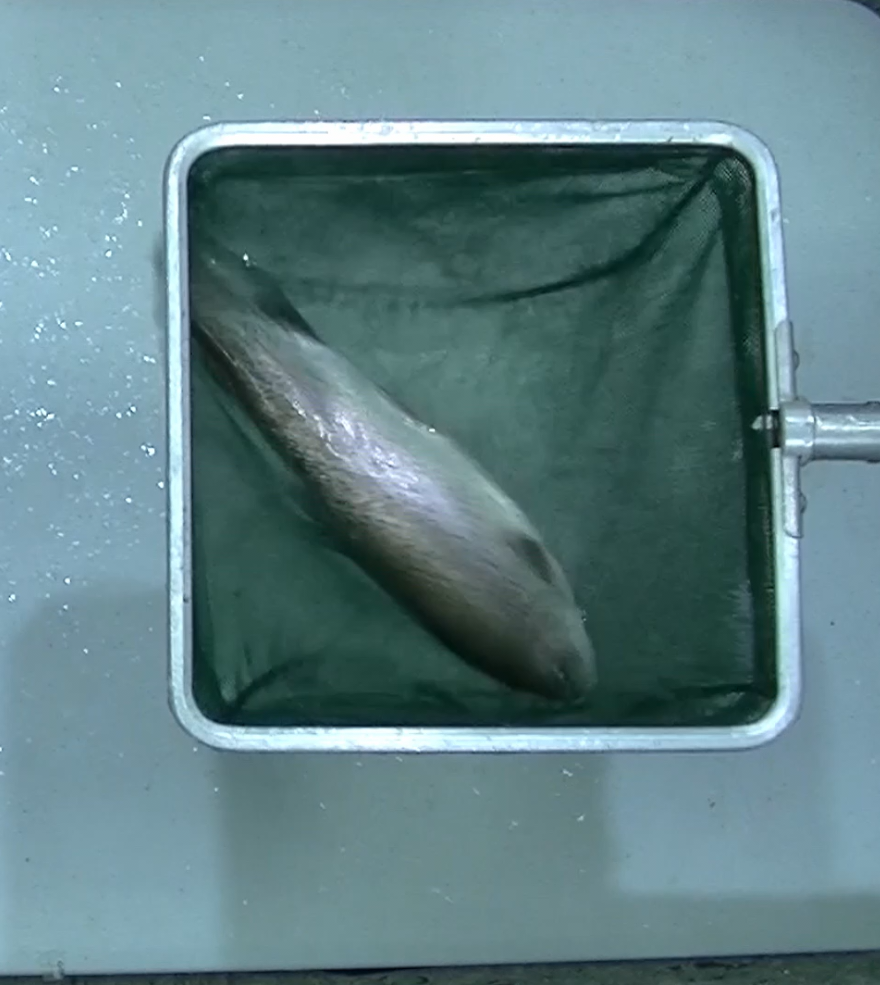
\includegraphics[width=0.8\textwidth]{images/6/SinOptical2.png}
                    \label{fig:SinOptical2}
                \end{subfigure}
                \begin{subfigure}[b]{0.25\textwidth}
                    \centering
                    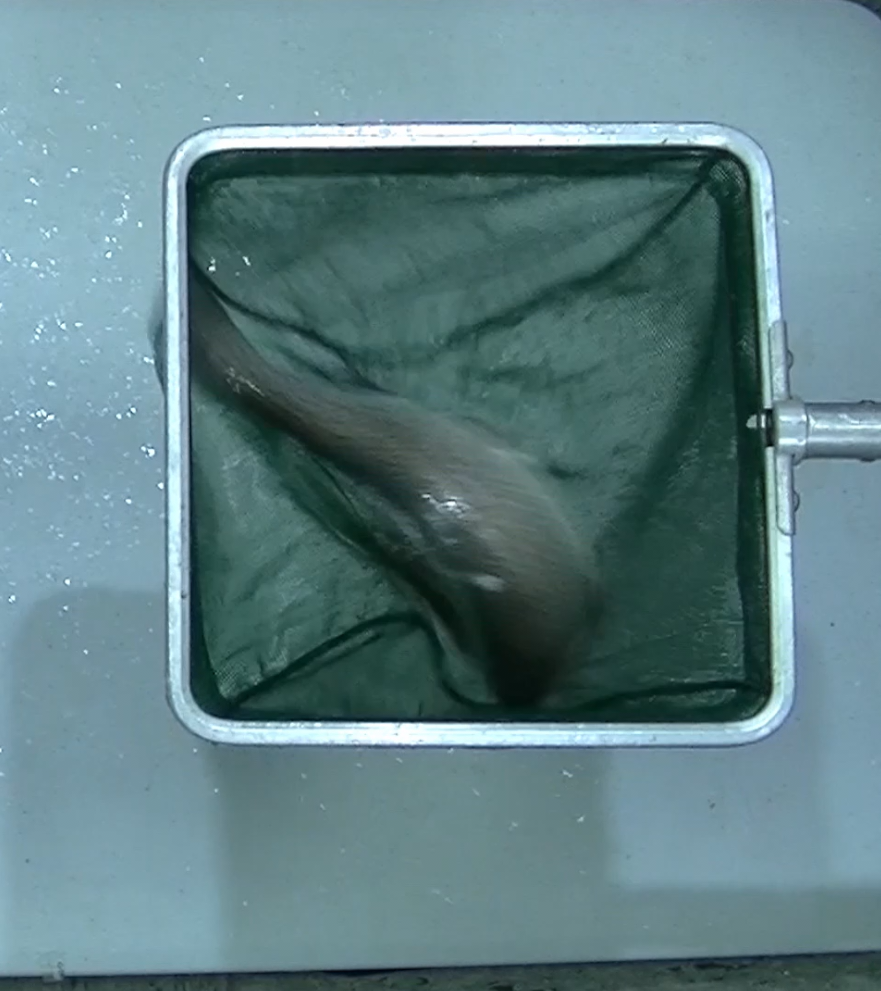
\includegraphics[width=0.8\textwidth]{images/6/SinOptical3.png}
                    \label{fig:SinOptical3}
                \end{subfigure}
                \begin{subfigure}[b]{0.25\textwidth}
                    \centering
                    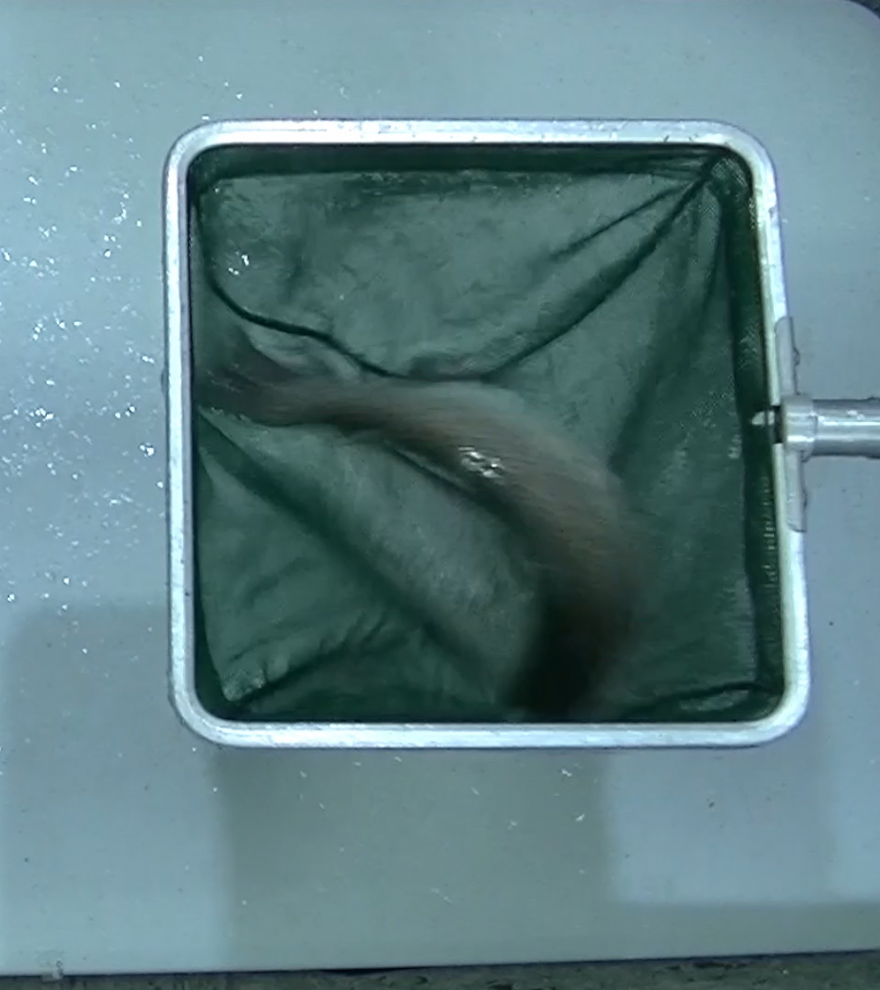
\includegraphics[width=0.78\textwidth]{images/6/SinOptical4.png}
                    \label{fig:SinOptical4}
                \end{subfigure}
                \caption{Fotogramas de entrada}
                \label{fig:FotogramasEntrada}
            \end{subfigure}
            \begin{subfigure}[b]{\textwidth}
                \centering
                \begin{subfigure}[b]{0.25\textwidth}
                    \centering
                    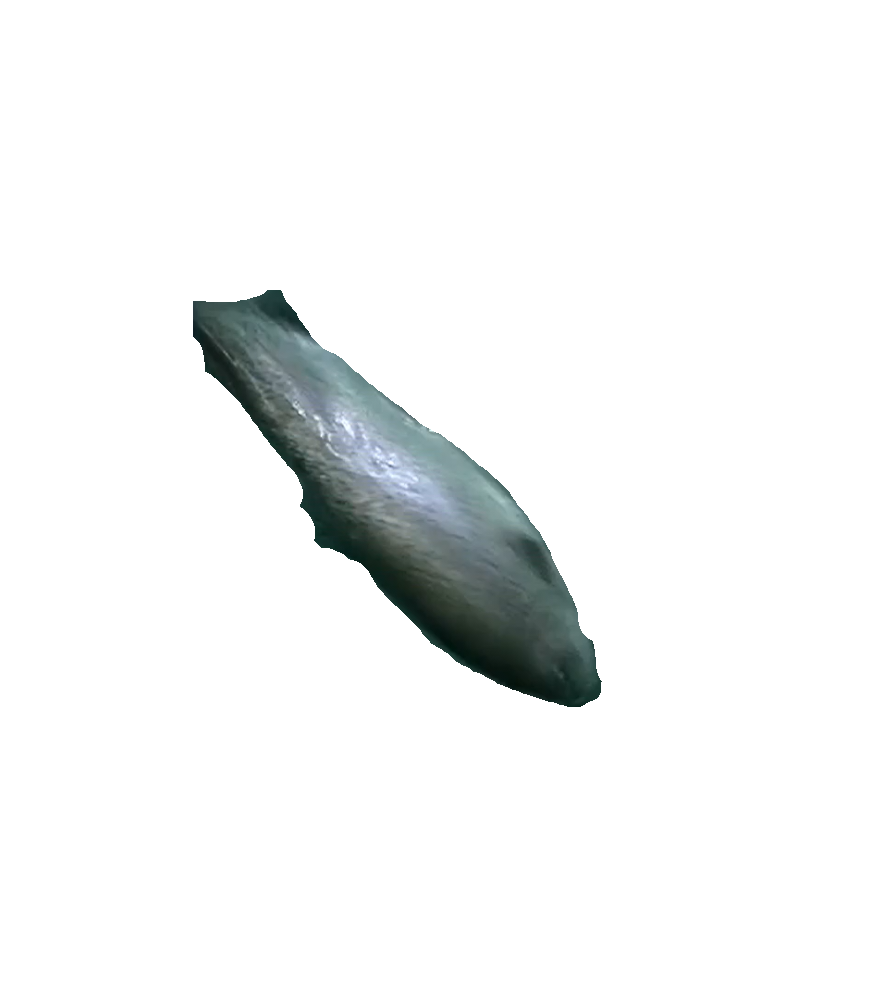
\includegraphics[width=0.8\textwidth]{images/6/Vacio2.png}
                    \label{fig:Vacio2}
                \end{subfigure}
                \begin{subfigure}[b]{0.25\textwidth}
                    \centering
                    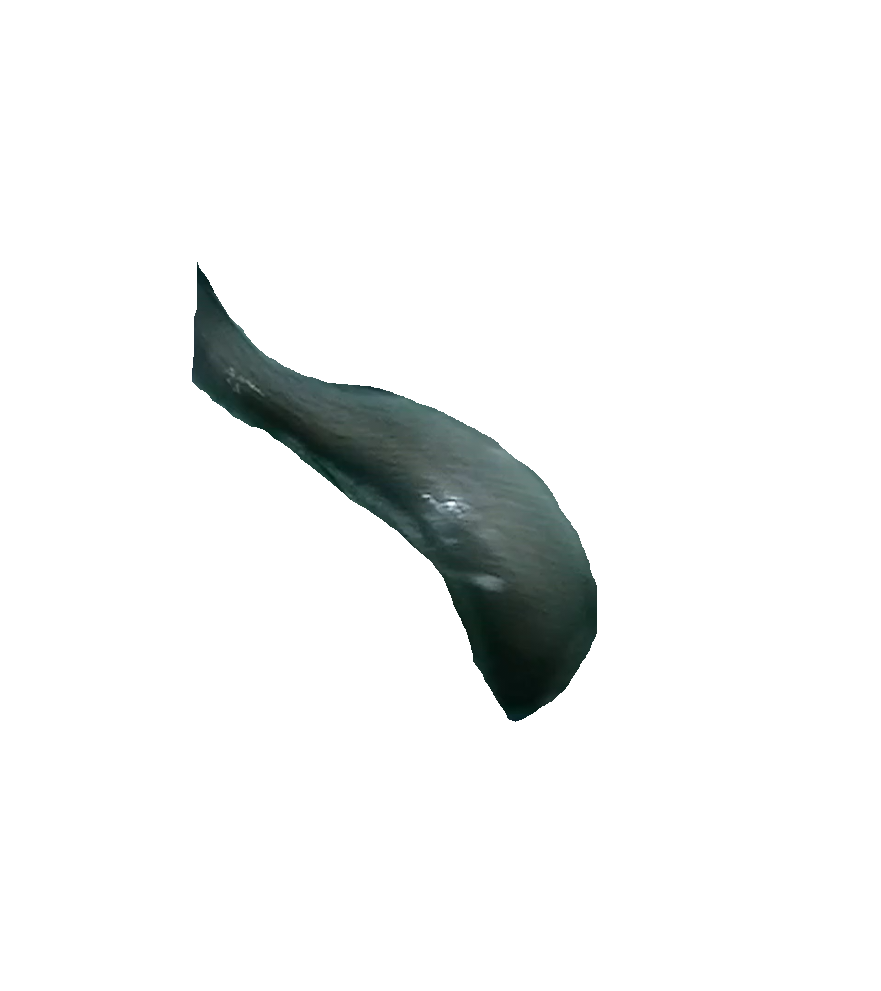
\includegraphics[width=0.8\textwidth]{images/6/Vacio3.png}
                    \label{fig:Vacio3}
                \end{subfigure}
                \begin{subfigure}[b]{0.25\textwidth}
                    \centering
                    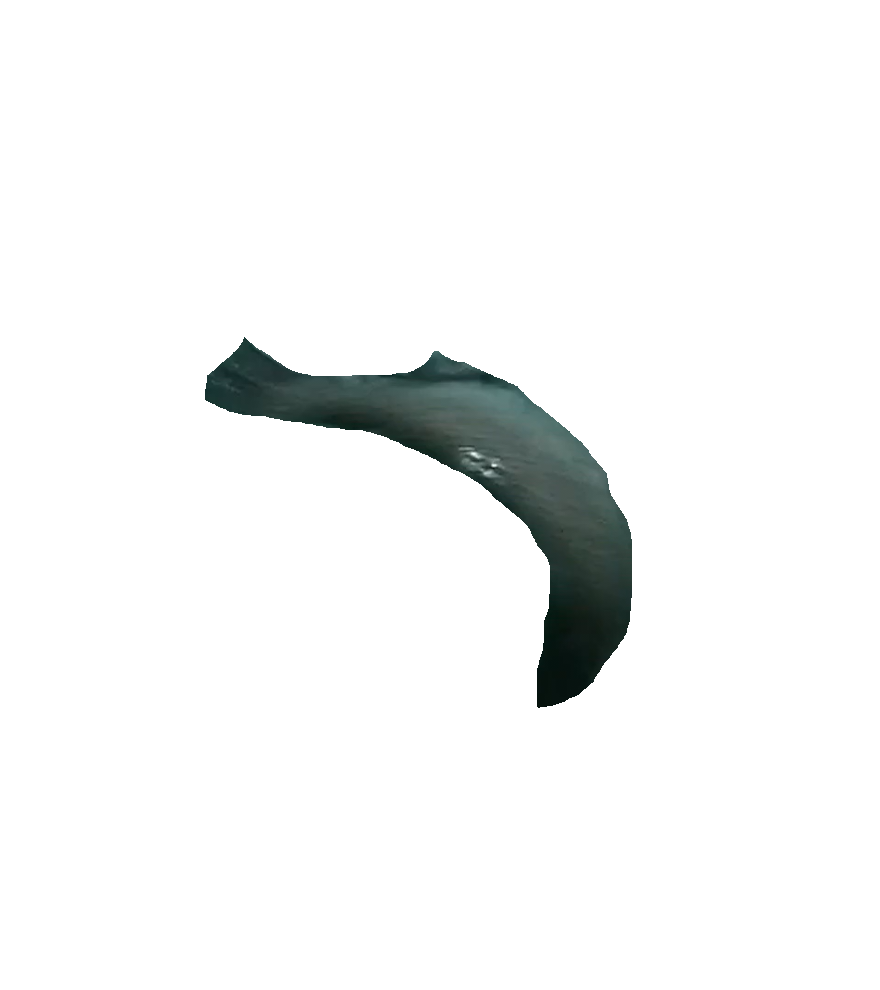
\includegraphics[width=0.8\textwidth]{images/6/Vacio4.png}
                    \label{fig:Vacio4}
                \end{subfigure}
                \caption{Fotogramas con el fondo eliminado}
                \label{fig:FotogramasSilueta}
            \end{subfigure}
            \begin{subfigure}[b]{\textwidth}
                \centering
                \begin{subfigure}[b]{0.25\textwidth}
                    \centering
                    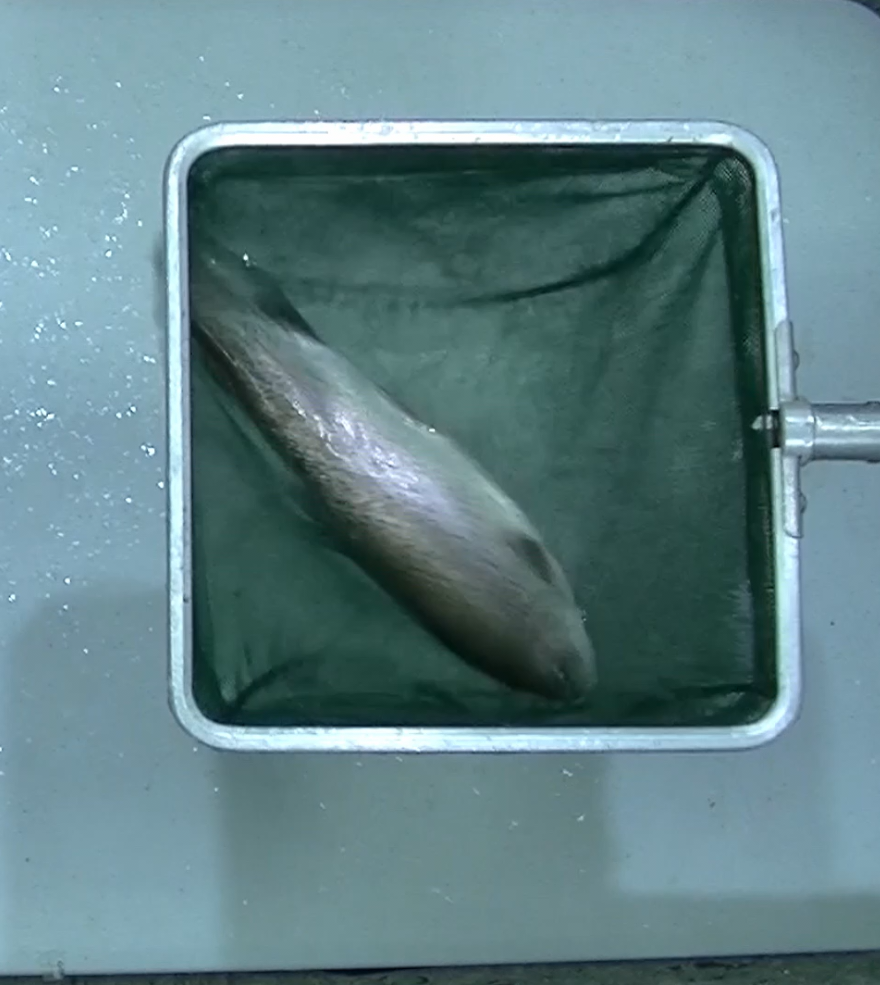
\includegraphics[width=0.8\textwidth]{images/6/SinOptical2.png}
                    \label{fig:Opt2}
                \end{subfigure}
                \begin{subfigure}[b]{0.25\textwidth}
                    \centering
                    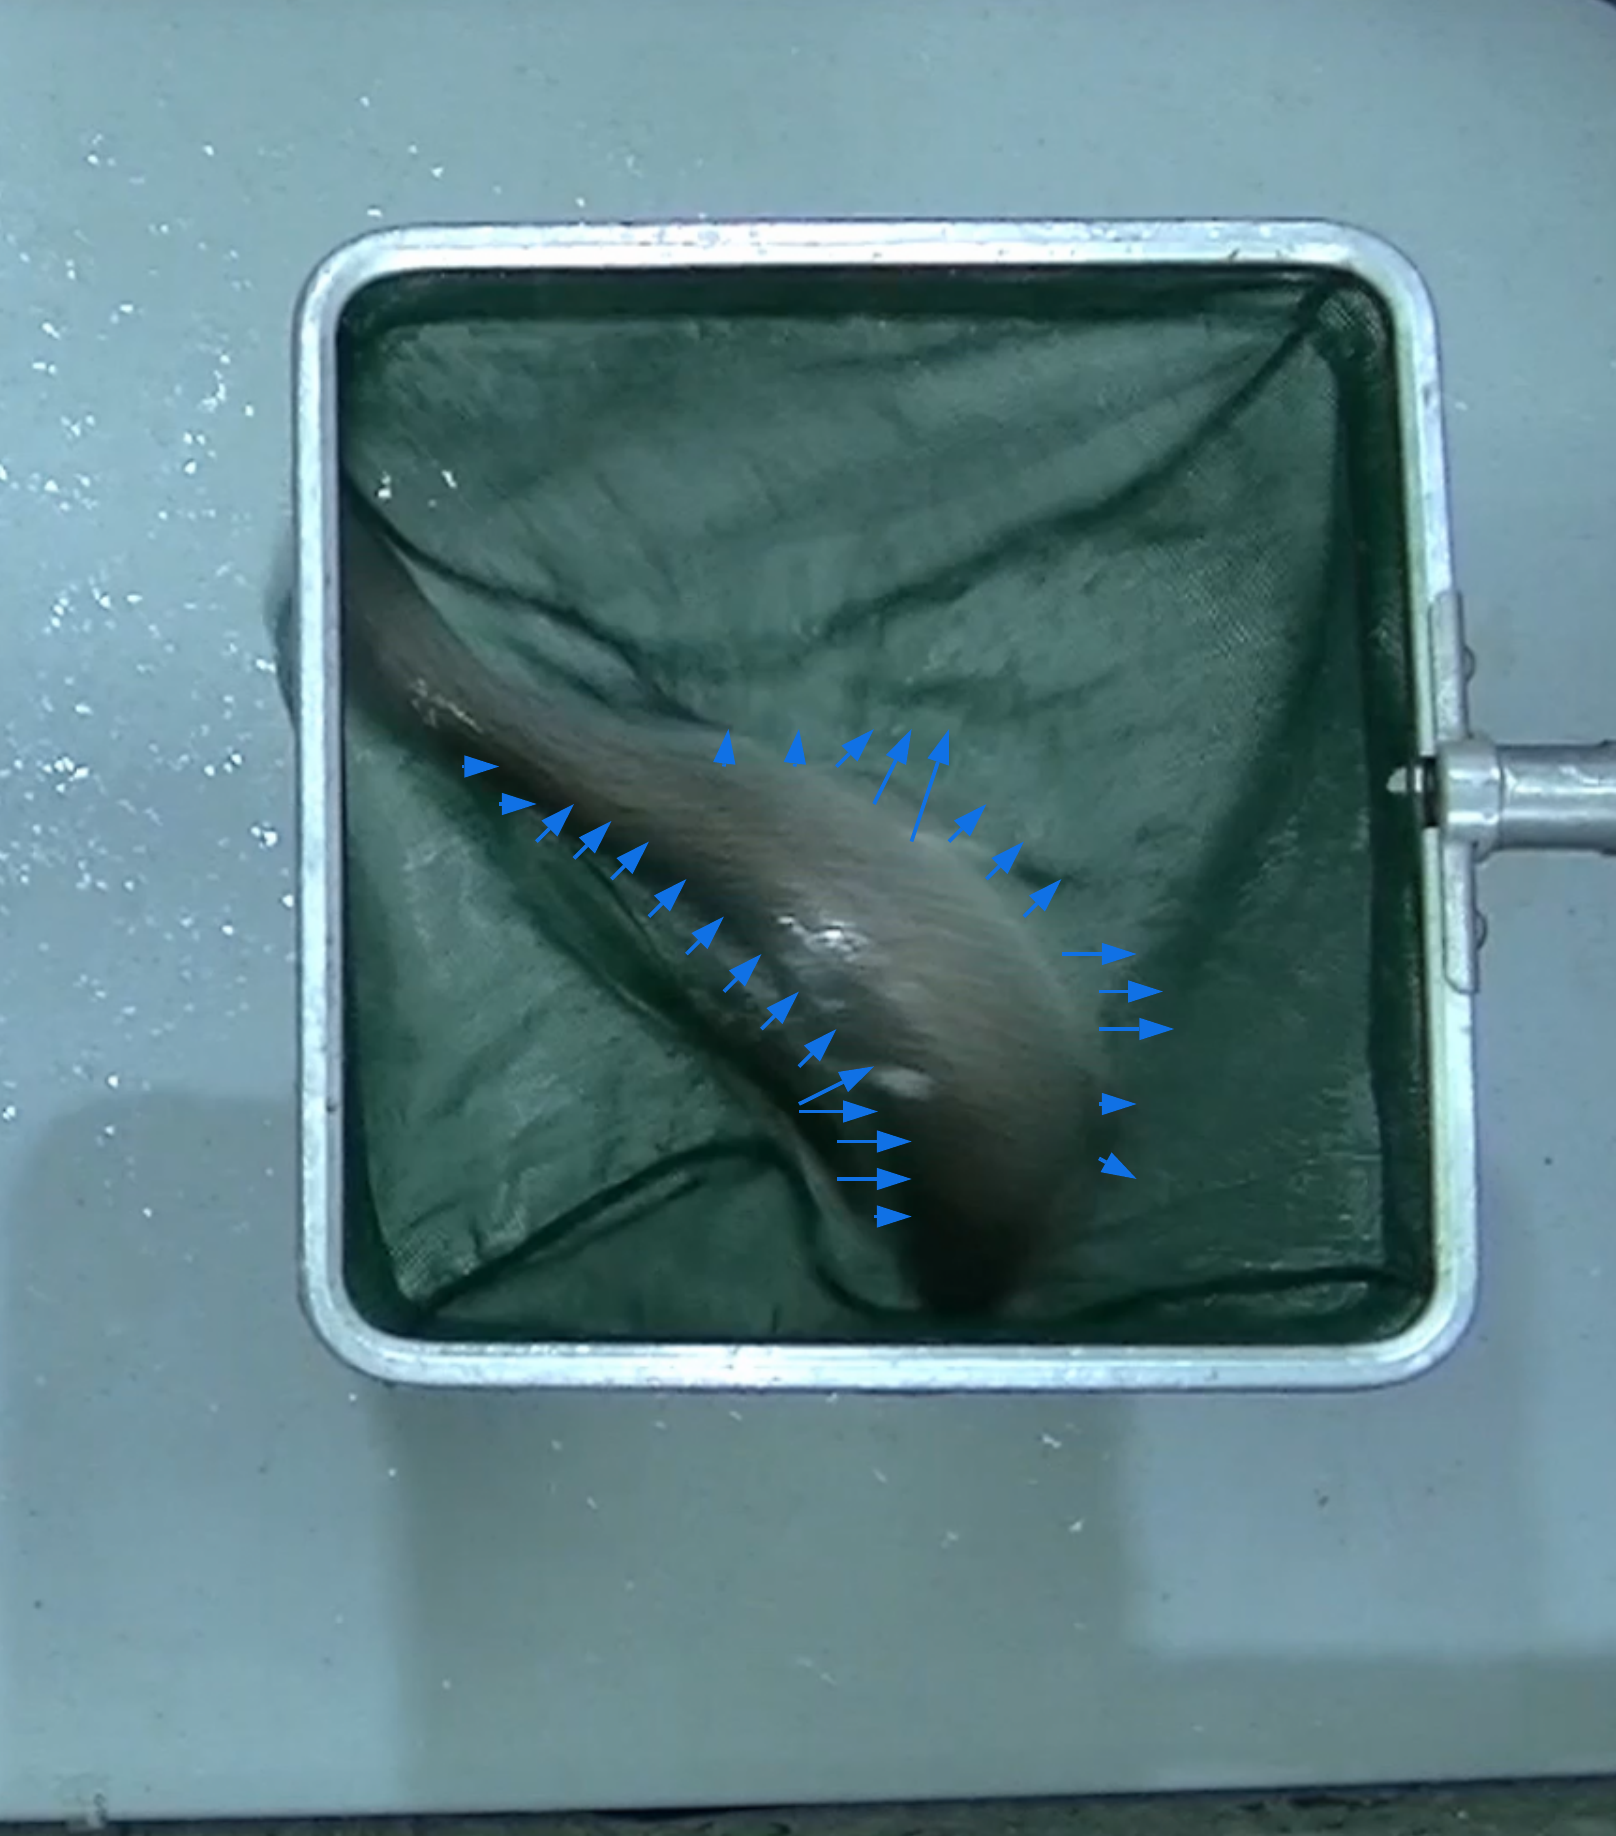
\includegraphics[width=0.8\textwidth]{images/6/ConOptical3.png}
                    \label{fig:Opt3}
                \end{subfigure}
                \begin{subfigure}[b]{0.25\textwidth}
                    \centering
                    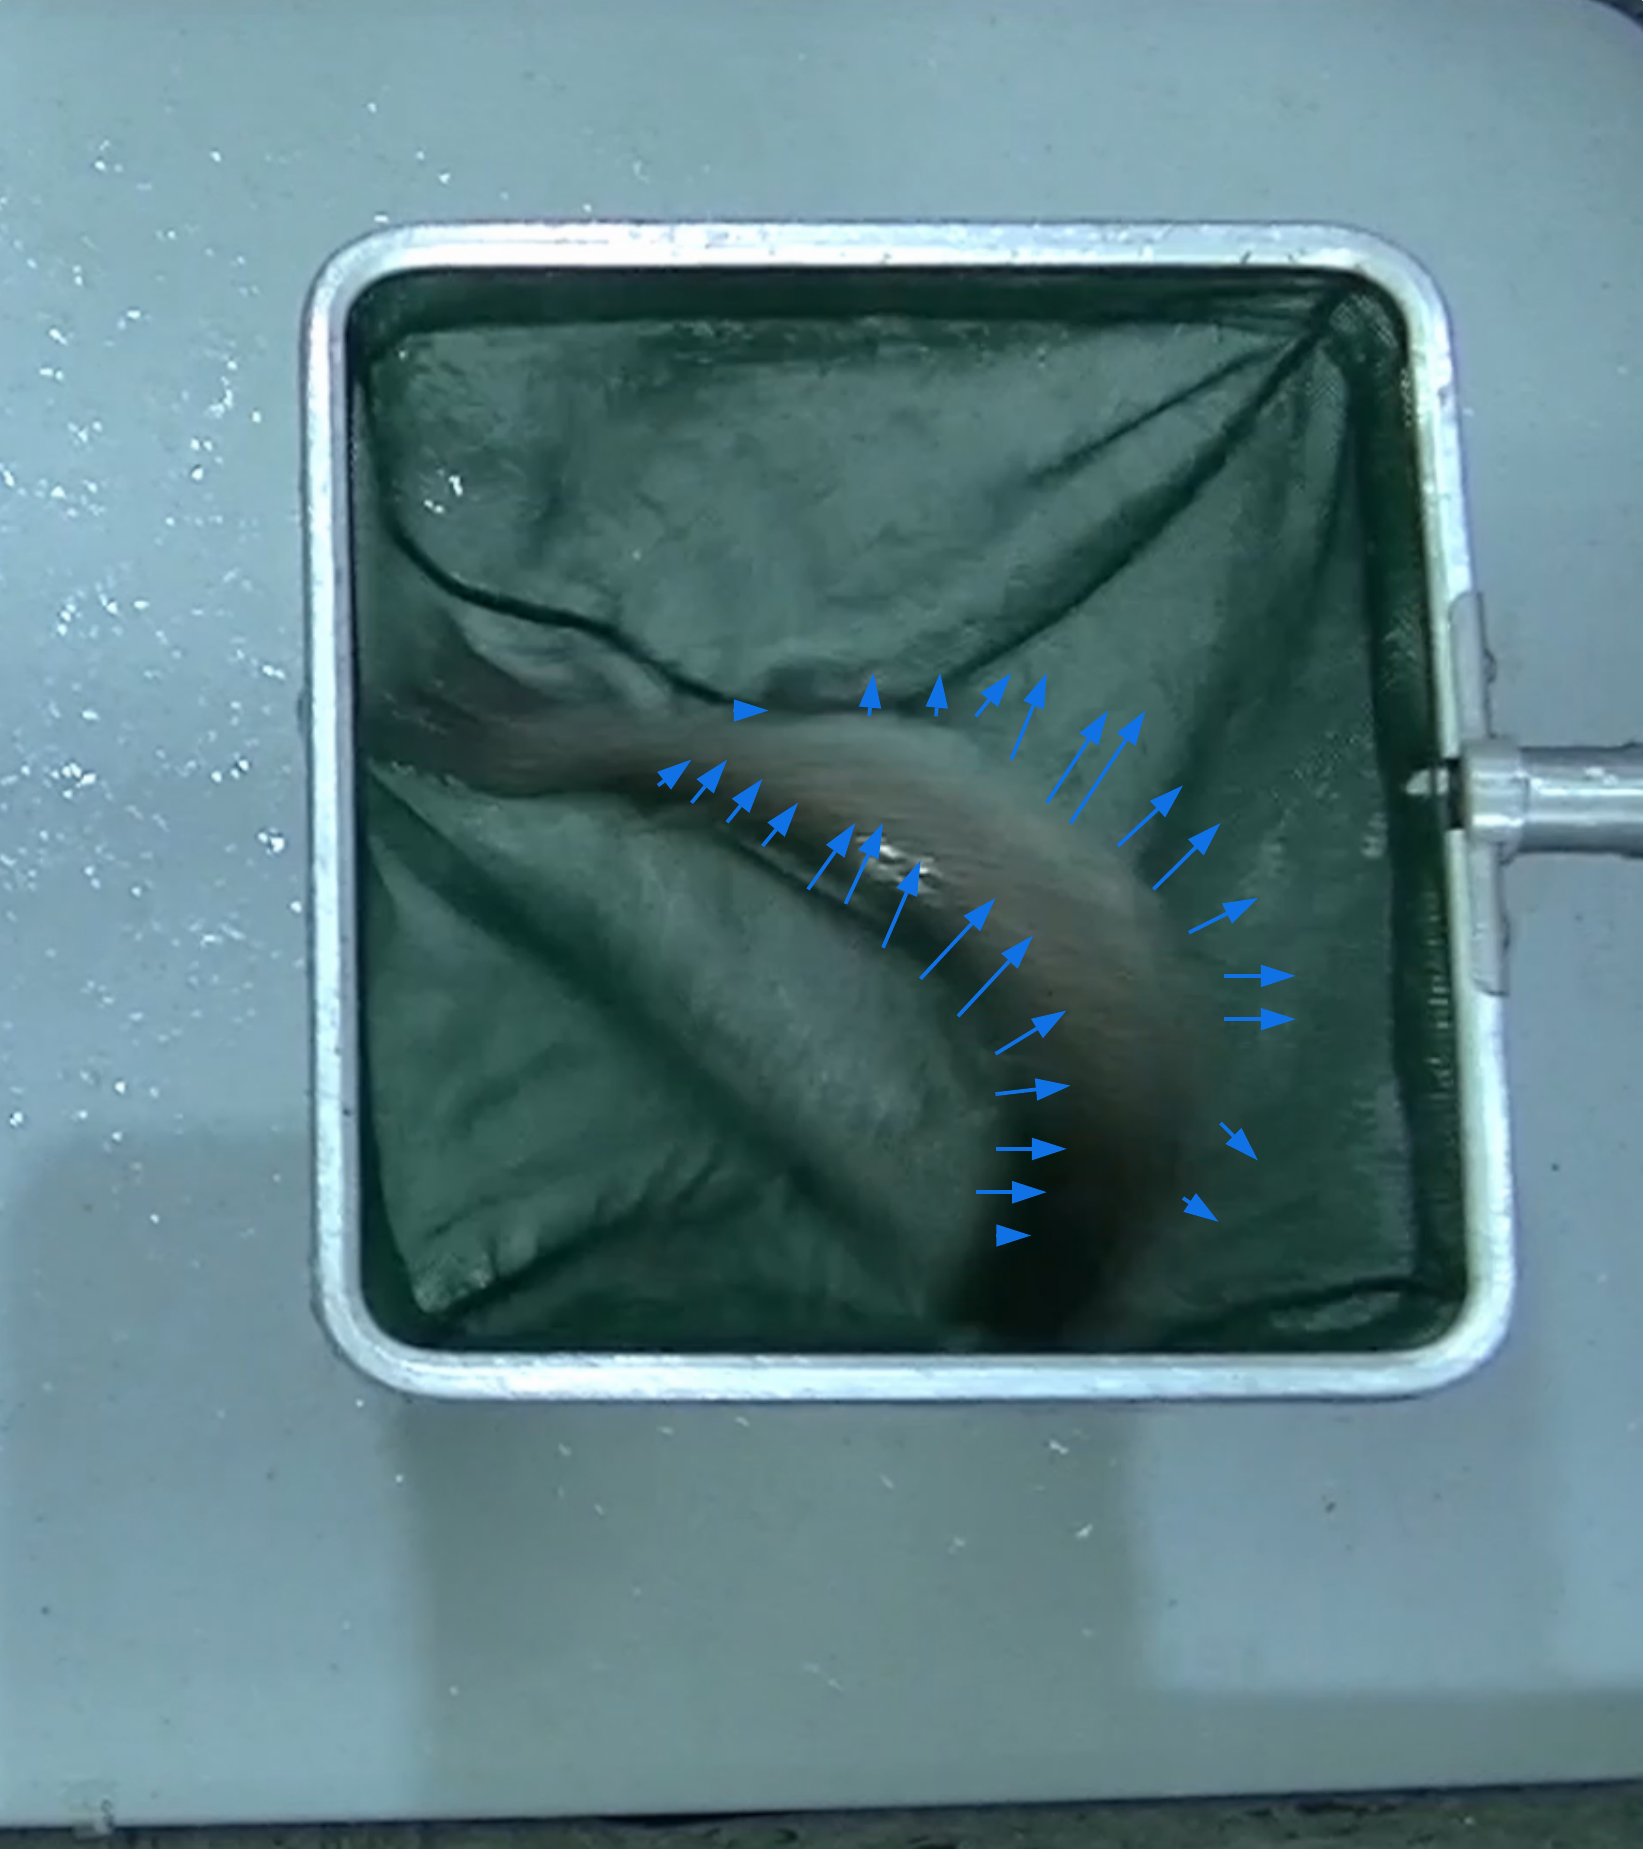
\includegraphics[width=0.8\textwidth]{images/6/ConOptical4.png}
                    \label{fig:Opt4}
                \end{subfigure}
                \caption{Fotogramas con el fondo eliminado}
                \label{fig:FotogramasSalidaOF}
            \end{subfigure}
    \caption{Idea general basada en \texttt{OpticalFlow} para el módulo de procesamiento del video}
    \label{fig:IdeaOF}
    \end{figure}

    Como se puede observar, la idea es obtener un conjunto de vectores en el contorno del pez que nos permitan 
    saber diferentes datos:
    \begin{itemize}
        \item Si se ha movido o no: a través de la suma de todos los vectores y la obtención del 
        módulo del vector global. Si este valor es mayor que cierto umbral, se podría indicar que está sucediendo 
        un movimiento entre los dos fotogramas.
        \item Hacia donde se ha movido: a través del análisis de la dirección del vector global; y si está ocurriendo 
        un movimiento, podemos decir hacia donde está ocurriendo y aportar más información.
    \end{itemize}

    \item \textbf{Solución basada en el uso de \textit{YOLO} como herramienta de análisis}: A través del uso de una \texttt{\acrshort{cnn}} 
    se procesa el video, obteniendo información sobre los objetos detectados como truchas.\newline
    Para realizar esto, hay que definir la tarea que realizaría la red:
    \begin{itemize}
        \item Clasificación: no es útil, ya que no aporta información sobre la posición de los objetos detectados en la imagen.
        \item Segmentación: puede ser útil, pero para entrenar la red en esta tarea, los datos etiquetados deben ser segmentos de la imagen. 
        Esto puede llevar demasiado tiempo y; como se verá más tarde, no es la única tarea que pueda aportar información para la automatización.
        \item Detección: es la más interesante, ya que nos permite conseguir unos tiempos de procesado por imagen muy bajos a la vez que nos da datos 
        relacionados con la posición y el tamaño aproximado de una caja rectangular que envuelva al pez.
    \end{itemize}
    
    Siendo la más viable la tarea de detección, se entrenaría un modelo \texttt{YOLO} para que sea capaz de detectar las truchas. Esto se realizaría 
    conformando un conjunto de datos de imágenes de truchas y sus respectivas etiquetas, que en este caso son dos esquinas de una caja (\texttt{Bounding Box}) que engloba el 
    objeto que se quiere detectar.\newline
    La red neuronal a la hora de realizar la inferencia nos devolvería objetos detectados de esa clase marcados con \texttt{Bounding Boxes} como se puede ver en el ejemplo de la \autoref{fig:IdeaYOLOGeneral}.
    
    A través de estas \texttt{Bounding Boxes}, podemos parametrizar un movimiento como la reducción del área o movimientos de la posición de la \texttt{Bounding Boxes}.

    \begin{figure}[H]
        \centering
        \begin{subfigure}[t]{0.39\textwidth}
            \centering
            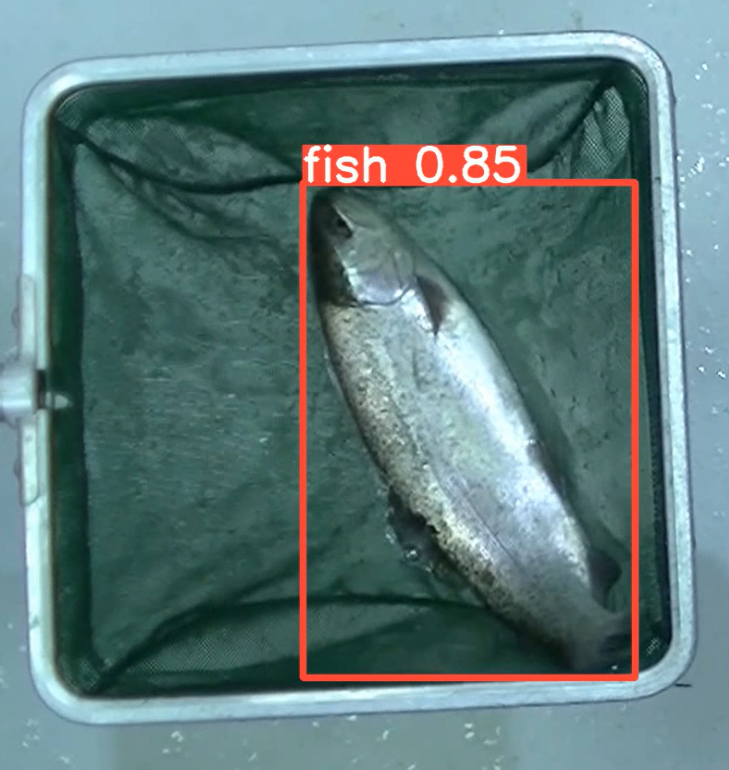
\includegraphics[width=0.8\textwidth]{images/6/EjemploYOLO.png}
            \caption{Imagen procesada por \texttt{YOLO}}
        \end{subfigure}
        \begin{subfigure}[t]{0.59\textwidth}
            \centering
            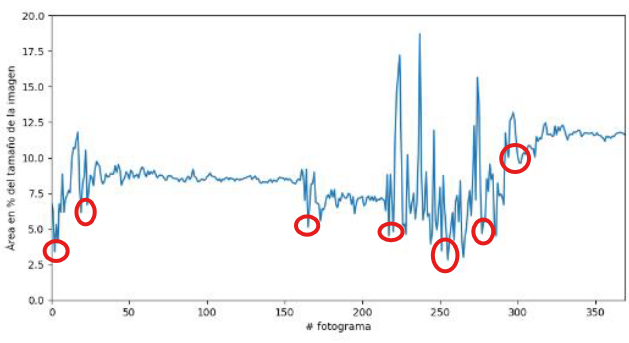
\includegraphics[width=0.99\textwidth]{images/6/YOLOEjemploResultados.png}
            \caption{Idea de estimación de movimiento a través de los resultados de las \texttt{Bounging Boxes}, marcando en rojo los movimientos}
        \end{subfigure}
        \caption{Idea general basada en \texttt{YOLO} para el módulo de procesamiento del video}
        \label{fig:IdeaYOLOGeneral}
    \end{figure}

    Hay que tener en cuenta que sería necesario hacer una validación de los entrenamientos realizados para conseguir cumplir con las necesidades. 
    Esto es debido a que al contrario que el \texttt{OpticalFlow}, las redes neuronales no son deterministas y dependiendo del fotograma sobre el que se realice inferencia, 
    podemos obtener resultados alejados de los esperados.
\end{enumerate}

\vspace{1\baselineskip}
Para decidir cuál método podía dar mejores resultados, se probaron las diferentes tecnologías aplicadas en el video \verb|23_NT_R1_J1_P7_8.mp4|. Este video dura 15 segundos y contiene dos peces, uno a 
la izquierda y otro a la derecha.

\clearpage
\subsubsection{Pruebas de concepto con \texttt{OpticalFlow}}

Para realizar las pruebas se utilizó el entorno de \texttt{MATLAB} en la versión \texttt{2023B}. En esta aplicación se disponen de 2 funciones principales 
que implementan análisis de flujo óptico: 
\begin{itemize}
    \item Método de Horn-Schunck: método de análisis denso (aplicado para todos los píxeles de la imagen).
    \item Método de Lucas-Kanade: método de análisis local (aplicado a áreas de píxeles que se asumen que tienen el mismo movimiento).
\end{itemize}

Ambas pruebas demostraron que los videos con los que se estaba trabajando tenían una tasa de fotogramas demasiado baja para la cantidad de movimiento que podía ocurrir entre fotogramas. 
Esto se puede observar en el flujo óptico percibido cuando suceden cambios bruscos del pez como en la \autoref{fig:HSOpticalFlow} para el método Horn-Schunck y en la \autoref{fig:LKOpticalFlow} 
para el método Lucas-Kanade.

\begin{figure}[H]
    \centering
    \begin{subfigure}[b]{0.49\textwidth}
        \centering
        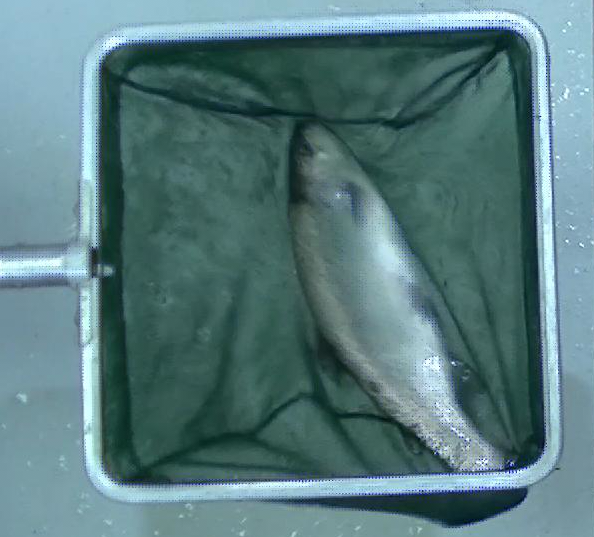
\includegraphics[width=0.95\textwidth]{images/6/6.2.1/HSIzquierda1.png}
    \end{subfigure}
    \begin{subfigure}[b]{0.49\textwidth}
        \centering
        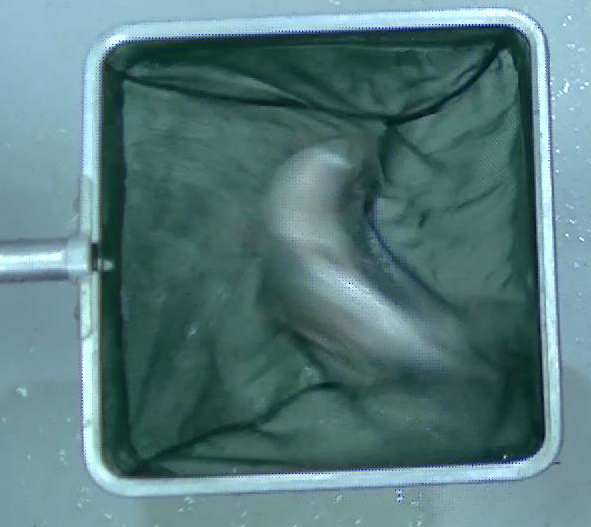
\includegraphics[width=0.95\textwidth]{images/6/6.2.1/HSIzquierda2.png}
    \end{subfigure}
    \caption{Flujo óptico detectado entre dos fotogramas por el método Horn-Schunck en los videos del \textit{NetText}}
    \label{fig:HSOpticalFlow}
\end{figure}

\begin{figure}[H]
    \centering
    \begin{subfigure}[b]{0.45\textwidth}
        \centering
        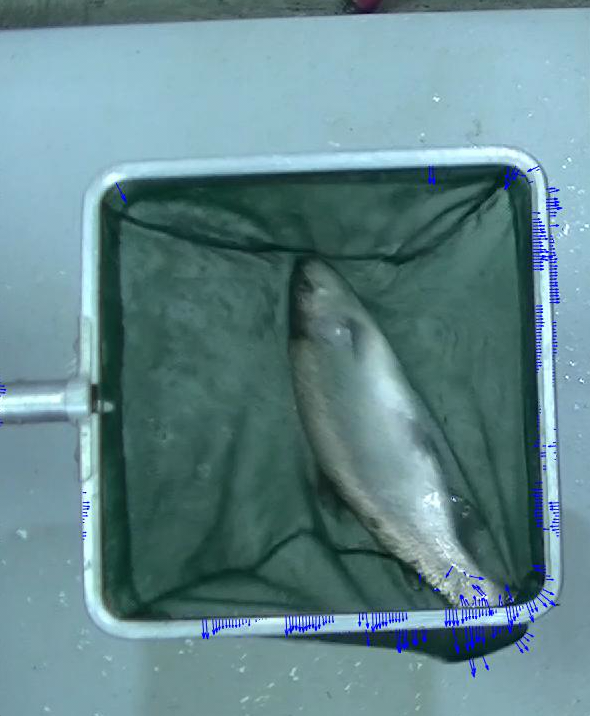
\includegraphics[width=0.8\textwidth]{images/6/6.2.1/LKIzquierda1.png}
    \end{subfigure}
    \begin{subfigure}[b]{0.45\textwidth}
        \centering
        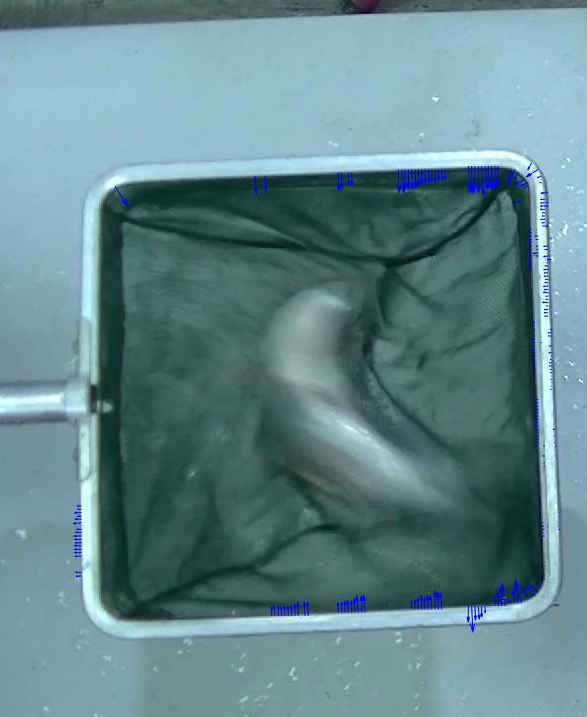
\includegraphics[width=0.8\textwidth]{images/6/6.2.1/LKIzquierda2.png}
    \end{subfigure}
    \caption{Flujo óptico detectado entre dos fotogramas por el método Lucas-Kanade en los videos del \textit{NetText}}
    \label{fig:LKOpticalFlow}
\end{figure}

El principal problema del método Horn-Schunck es que se ve muy afectado por el ruido, en el caso de este experimento, ese ruido aparece por el poco \texttt{bitrate} que tiene el video 
en comparación con la velocidad de movimiento que tienen las truchas. Aparte de esto, es un método computacionalmente muy costoso. en el caso de este video de 15 segundos tardó cerca de 10 
minutos en realizar el análisis completo del flujo óptico, lo cual incumple el requisito 18.

Vemos cierta mejoría usando el método de Lucas-Kanade, pero al realizar el análisis de forma local en zonas con similitudes, en cuanto la trucha hace un movimiento, el análisis deja de funcionar 
sobre la parte de la imagen en la que se sitúa la trucha. Aún siendo bastante rápido (sin llegar a ser tiempo real), esta situación elimina la posibilidad de utilizar este método para la 
parametrización del movimiento de la trucha.

En ambos métodos se ha comprobado que mejorarían los resultados aplicando umbralizaciones a la imagen. También sería necesario un preprocesado para delimitar la sección de 
imagen sobre la que es de interés realizar el análisis de flujo óptico (la zona de la red que contiene la trucha). Aún con lo comentado anteriormente, el único método que puede aportar algún 
tipo de información de manera consistente para todo el video es el método de Horn-Schunck.

\subsubsection{Pruebas de concepto con \texttt{YOLO}}

Para realizar esta prueba, creo un conjunto de datos con el que entrenar a través de fotogramas del video \verb|23_NT_R1_J1_P1_2.mp4|. Esto se realizó a través de la herramienta \texttt{\acrfullr{cvat}}.\newline
Esta herramienta de código abierto\cite{cvat.aicorporationComputerVisionAnnotation2023} es mantenida por los creadores de la librería \texttt{OpenCV}. Dispone de una versión online limitada al número de 
archivos que se pueden subir a \texttt{500 MB} y en otros aspectos, pero también dispone de una versión desplegable por \texttt{Docker}. Uno de sus puntos fuertes y el motivo de su uso en este trabajo es 
la compatibilidad con muchos formatos de exportación de etiquetas.

Como parte de este proyecto y como sistema que sirviese de soporte para guardar todos los conjuntos de datos necesarios, se desplegó como contenedor en el servidor \acrfullr{nas} del \acrfullr{gamma}.

Con esta aplicación se realizó el etiquetado de 24 imágenes para realizar un primer entrenamiento, el conjunto de datos se dividió de la siguiente manera:
\begin{itemize}
    \item 16 imágenes para el conjunto de entrenamiento.
    \item 4 imágenes para el conjunto de validación.
    \item 4 imágenes para el conjunto de pruebas
\end{itemize}

Posteriormente se realizó el entrenamiento de la red neuronal \texttt{YOLOv8} versión \texttt{nano}, que es la más pequeña y rápida de entrenar

\vspace{3\baselineskip}
Hay que hablar del entrenamiento, conjunto de datos usado, verificación de resultados, tiempo de procesado, viabilidad de solución, estimación de movimiento a través de las áreas de las bounding 
boxes.

Finalmente hablar de los resultados publicados en el congreso de Álvaro y su respectiva cita.

\clearpage
\subsection{Pruebas de desarrollo: sistema \texttt{StandAlone} con \texttt{YOLO}}



\clearpage
\subsection{Desarrollo de aplicación completa}
\subsection{Desarrollo de aplicación completa}

El siguiente objetivo del trabajo fue desarrollar una aplicación completa que permitiese a los usuarios obtener los resultados de forma fácil. Esto fue decidido principalmente por dos razones:

\begin{itemize}
    \item Era necesario cumplir el requisito que afecta al nivel de conocimiento necesario para manejar la herramienta. Con una aplicación que tuviese interfaz gráfica, se podría manejar mucho mejor que 
    obligar al usuario a usar una consola de comandos o a conocer como funcionar las diferentes dependencias de las librerías usadas.
    \item Servía como oportunidad para mejorar los servicios que era capaz de proporcionar el sistema, además de poder diseñar la aplicación para poder aprovechar de forma eficiente los recursos del 
    \texttt{HardWare}.
\end{itemize}

Para desarrollar esta aplicación primero se seleccionó la librería de \acrfullr{gui}. Este paso fue importante porque existen muchas posibles librerías en el entorno de \texttt{Python}, pero cada una 
aporta diferentes utilidades y abstracciones, siendo las más comunes:
\begin{itemize}
    \item \texttt{TKinter}: es el \texttt{framework} más usado en \texttt{Python}. Es una librería simple y que no se suele usar para manejar datos multimedia, ya que es muy simple.
    \item \texttt{PyQT}: librería que internamente usa el \texttt{framework} \texttt{QT}. Es mucho más potente y capaz de manejar videos y elementos complejos.
    \item \texttt{Kivy}: librería pensada para el desarrollo de aplicaciones móviles.
    \item \texttt{PySimpleGUI}: es una librería \texttt{wrapper} sobre \texttt{Tkinter} y similares, por lo tanto es muy simple, pero limita mucho.
    \item \texttt{Remi}: se usa para crear interfaces web.
    \item \texttt{DearPyGUI}\cite{HoffstadtDearPyGuiDear}: librería muy reciente que se centra en dar al usuario la máxima eficiencia posible, usando aceleración \texttt{HardWare} a través de \texttt{OpenGL}.
\end{itemize}

\vspace{2\baselineskip}

Al estar trabajando con redes neuronales, queremos que la interfaz gráfica utilice la menor cantidad de recursos posible y de la manera más eficiente. Además, como se verá en los siguientes puntos, 
se implementaron partes multimedia en la aplicación, por lo tanto fue necesaria una librería centrada en la eficiencia, lo cual dejaba como posibles opciones 
\texttt{PyQT} y \texttt{DearPyGUI}, sin embargo por motivos personales del autor, la librería seleccionada fue \texttt{DearPyGUI}.

La selección se debe a la experiencia del autor en otros trabajos con la misma librería para realizar aplicaciones de manejo de cámaras IP. Al conocer ya la librería, se reducirían 
los posibles problemas y la necesidad de mirar documentación. Además de esta experiencia pasada, quedó patente que \texttt{DearPyGUI} es capaz de manejar los recursos del ordenador de forma muy eficiente.

\clearpage
\subsubsection{Diseño de interfaz para la aplicación}

Para realizar el diseño de la aplicación, se diseñó a través de la herramienta \texttt{DrawIO}, un esquema general del flujo y ventanas de la aplicación (completo en el \hyperref[esquema:FlujoVentanas]{anexo c}).\newline
Usando este esquema como idea general, se fue desarrollando la aplicación poco a poco, desde la ventana inicial hasta la ventana de datos

\begin{itemize}
    \item Ventana inicial de la interfaz
\end{itemize}
\newpage
\thispagestyle{abstract}
\mbox{}
\newpage
\section{VALIDACIÓN DE RESULTADOS}

Como proyecto de ingeniería, se debe llevar a cabo un análisis de cumplimiento de los requerimientos del sistema desarrollado a través de métricas. Para la validación se van a evaluar las 
diferentes partes del trabajo.

Primeramente, a través del entrenamiento de la red neuronal, se ha buscado minimizar el error asociado a las \texttt{Bounding Boxes}, ya que el sistema usa esto como base para calcular movimientos. 
En este sentido, con el último conjunto de datos y 600 épocas, se han conseguido alcanzar un error de \texttt{0.2} y \texttt{0.9} en el conjunto de datos de entrenamiento y validación respectivamente, siendo 
este resultado uno de los mejores de todos los entrenamientos y con un conjunto de validación mucho más realista. Los resultados de la validación se pueden ver en la \autoref{fig:ValidacionRed}.

\begin{figure}[H]
    \centering
    \begin{subfigure}[b]{0.7\textwidth}
        \centering
        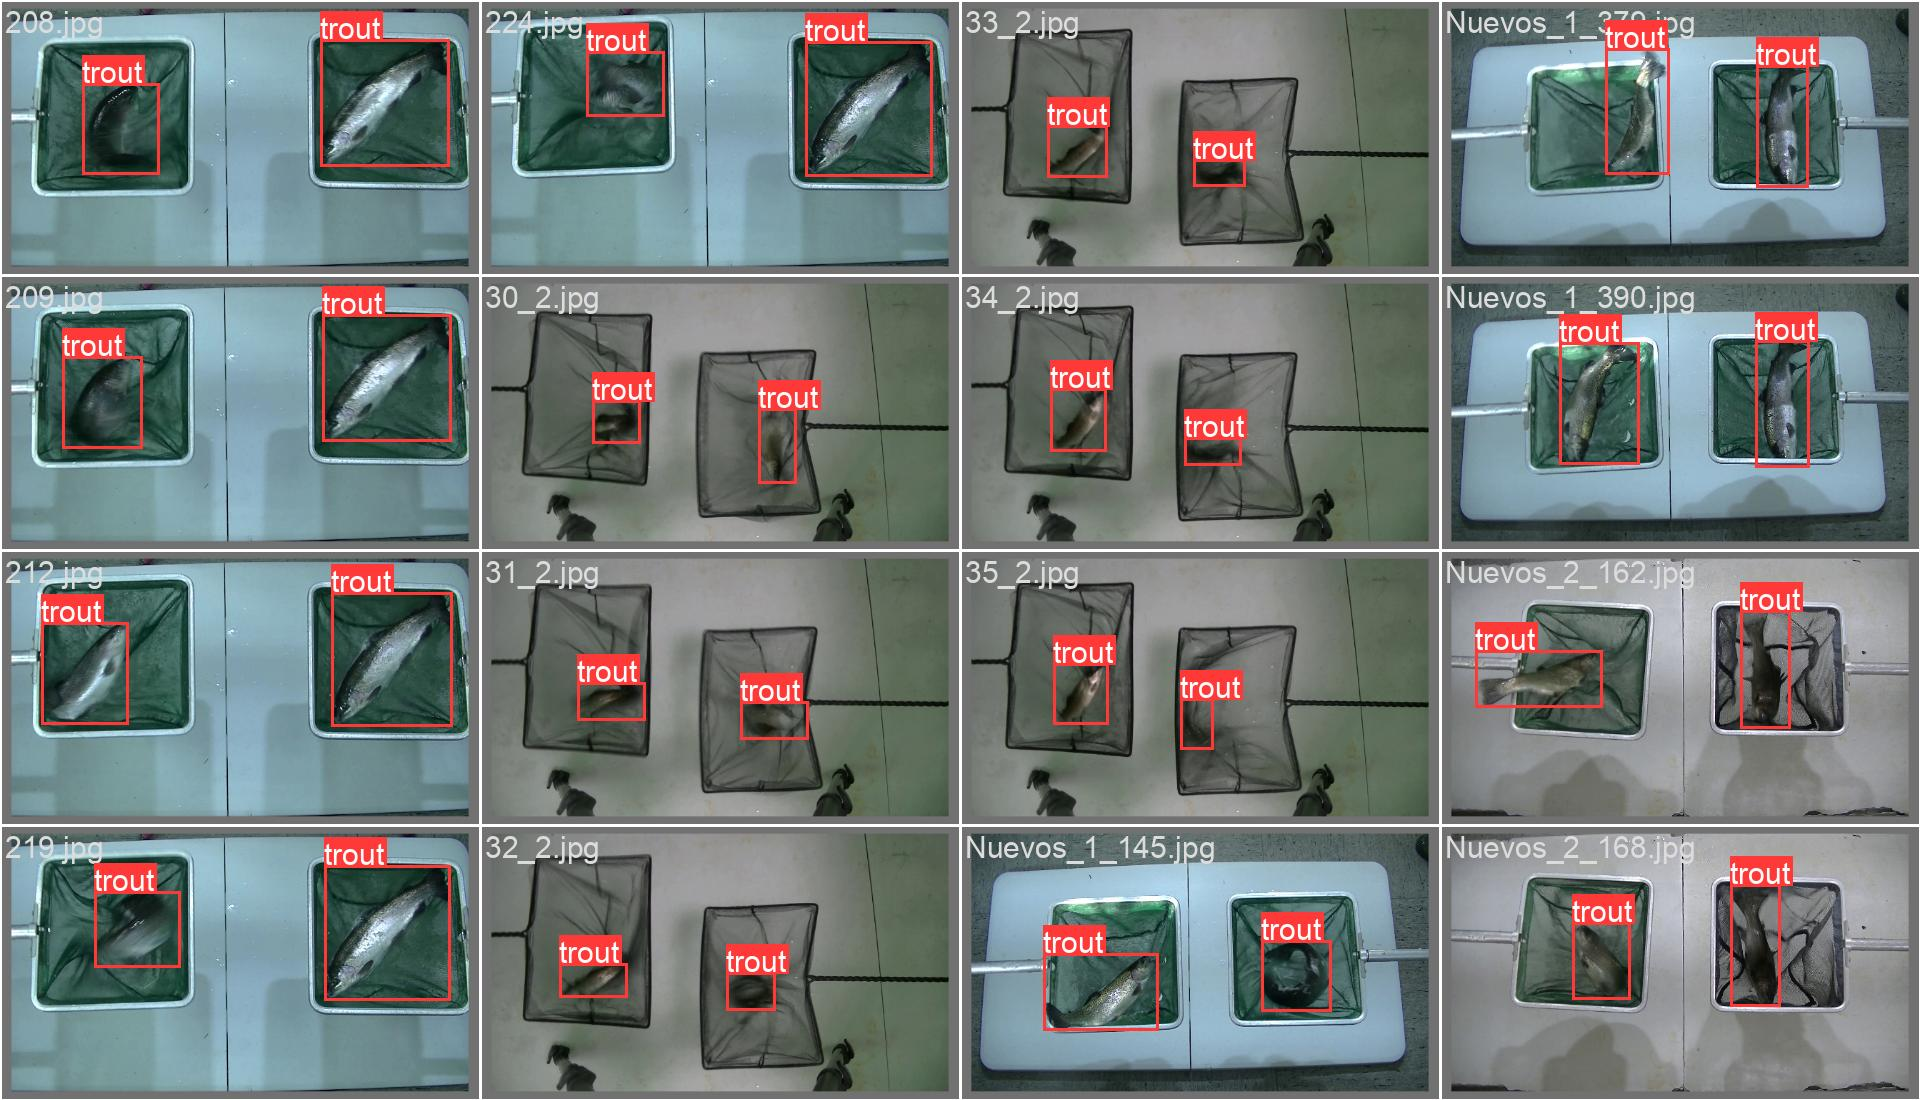
\includegraphics[width=0.95\textwidth]{images/7/labels.jpg}
        \caption{Etiquetas del conjunto de validación final}
    \end{subfigure}
    \begin{subfigure}[b]{0.7\textwidth}
        \centering
        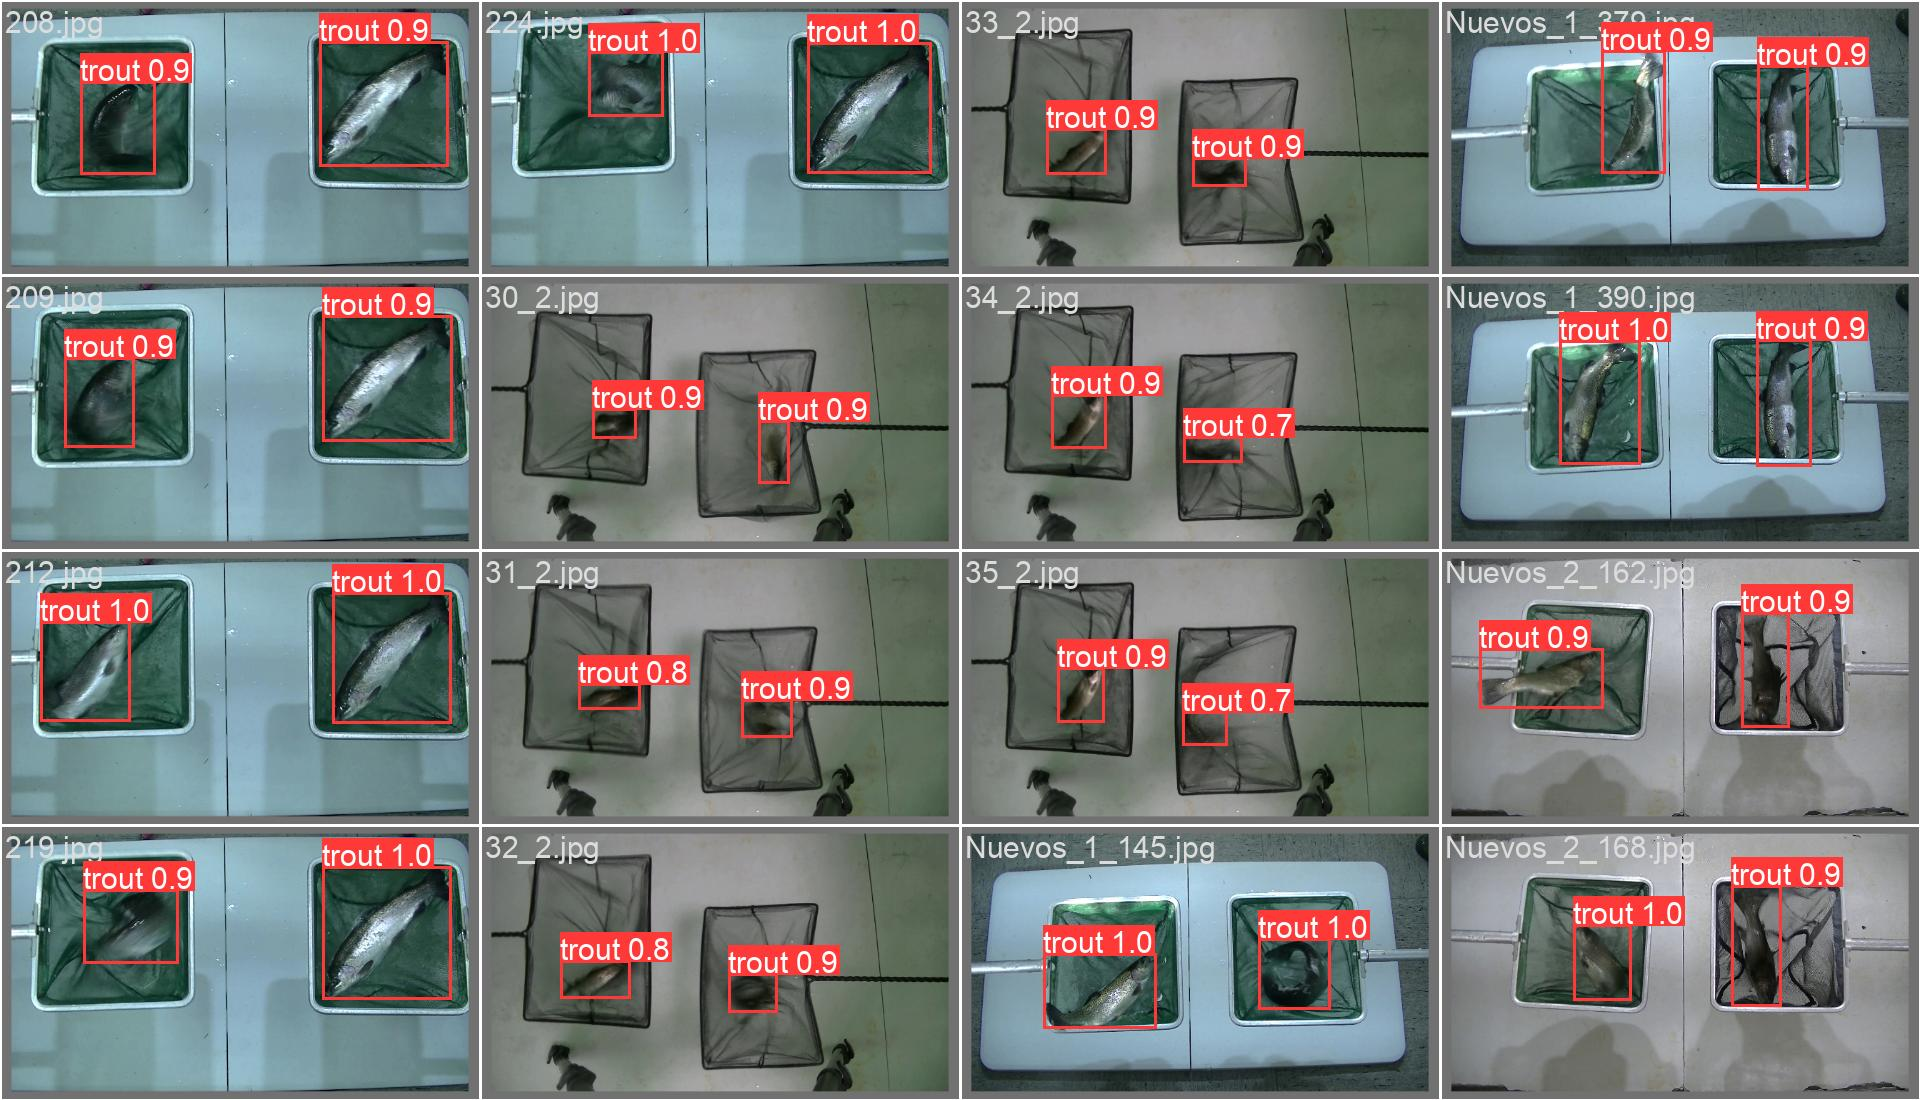
\includegraphics[width=0.95\textwidth]{images/7/pred.jpg}
        \caption{Predicciones sobre el conjunto de validación final}
    \end{subfigure}
    \caption{Resultados finales sobre el conjunto de validación}
    \label{fig:ValidacionRed}
\end{figure}

Aparte de los resultados de validación, como ya se ha dicho en el trabajo y se puede ver en \hyperref[train:final]{las gráficas de resultados del anexo c}, se buscaba maximizar otras métricas como son 
el \texttt{recall} a niveles altos para obtener una cantidad elevada de verdaderos 
positivos. Finalmente, también se ha conseguido alcanzar una precisión \texttt{mAP50-95} muy elevada (0.82) teniendo en cuenta la variabilidad del conjunto de datos, lo cual nos indica una precisión 
general de la red muy buena.

\clearpage

Seguidamente, se realizó la validación del número de movimientos utilizando las etiquetas proporcionadas por los investigadores como ya se comentó en el análisis de los datos. Para esto, se utilizó la aplicación en el conjunto de 
videos del \textit{NetText}1 al \textit{NetText}4, a través de las jaulas 1 a la 4, excluyendo los videos que contenían el primer y el segundo pez (ya que para entrenamiento se han usado los videos \verb|23_NT_R1_J1_P1_2|, \verb|23_NT_R2_J1_P1_P2|, \verb|23_NT_R3_J1_P1_P2| 
y \verb|23_NT_R3_J2_P1_P2|).

Al principio de este trabajo, se pensó que las etiquetas de los investigadores eran incorrectas, ya que al revisar manualmente el movimiento de los videos, el número de movimientos no era ni cercano. Sin embargo, según se realizaba el 
análisis de los videos, se observó que extrañamente, las etiquetas asociadas a la trucha izquierda eran más similares a los movimientos de la derecha y viceversa.

Analizando los coeficientes de correlación y graficando la relación lineal de los datos de la \autoref{fig:EtiquetadosMal}, se observó que efectivamente, los datos etiquetados simplemente no estaban en \acrshort{ltr}, sino al revés. Por lo tanto se arreglaron 
los datos para la .

\begin{figure}[H]
    \centering
    \begin{subfigure}[b]{0.7\textwidth}
        \centering
        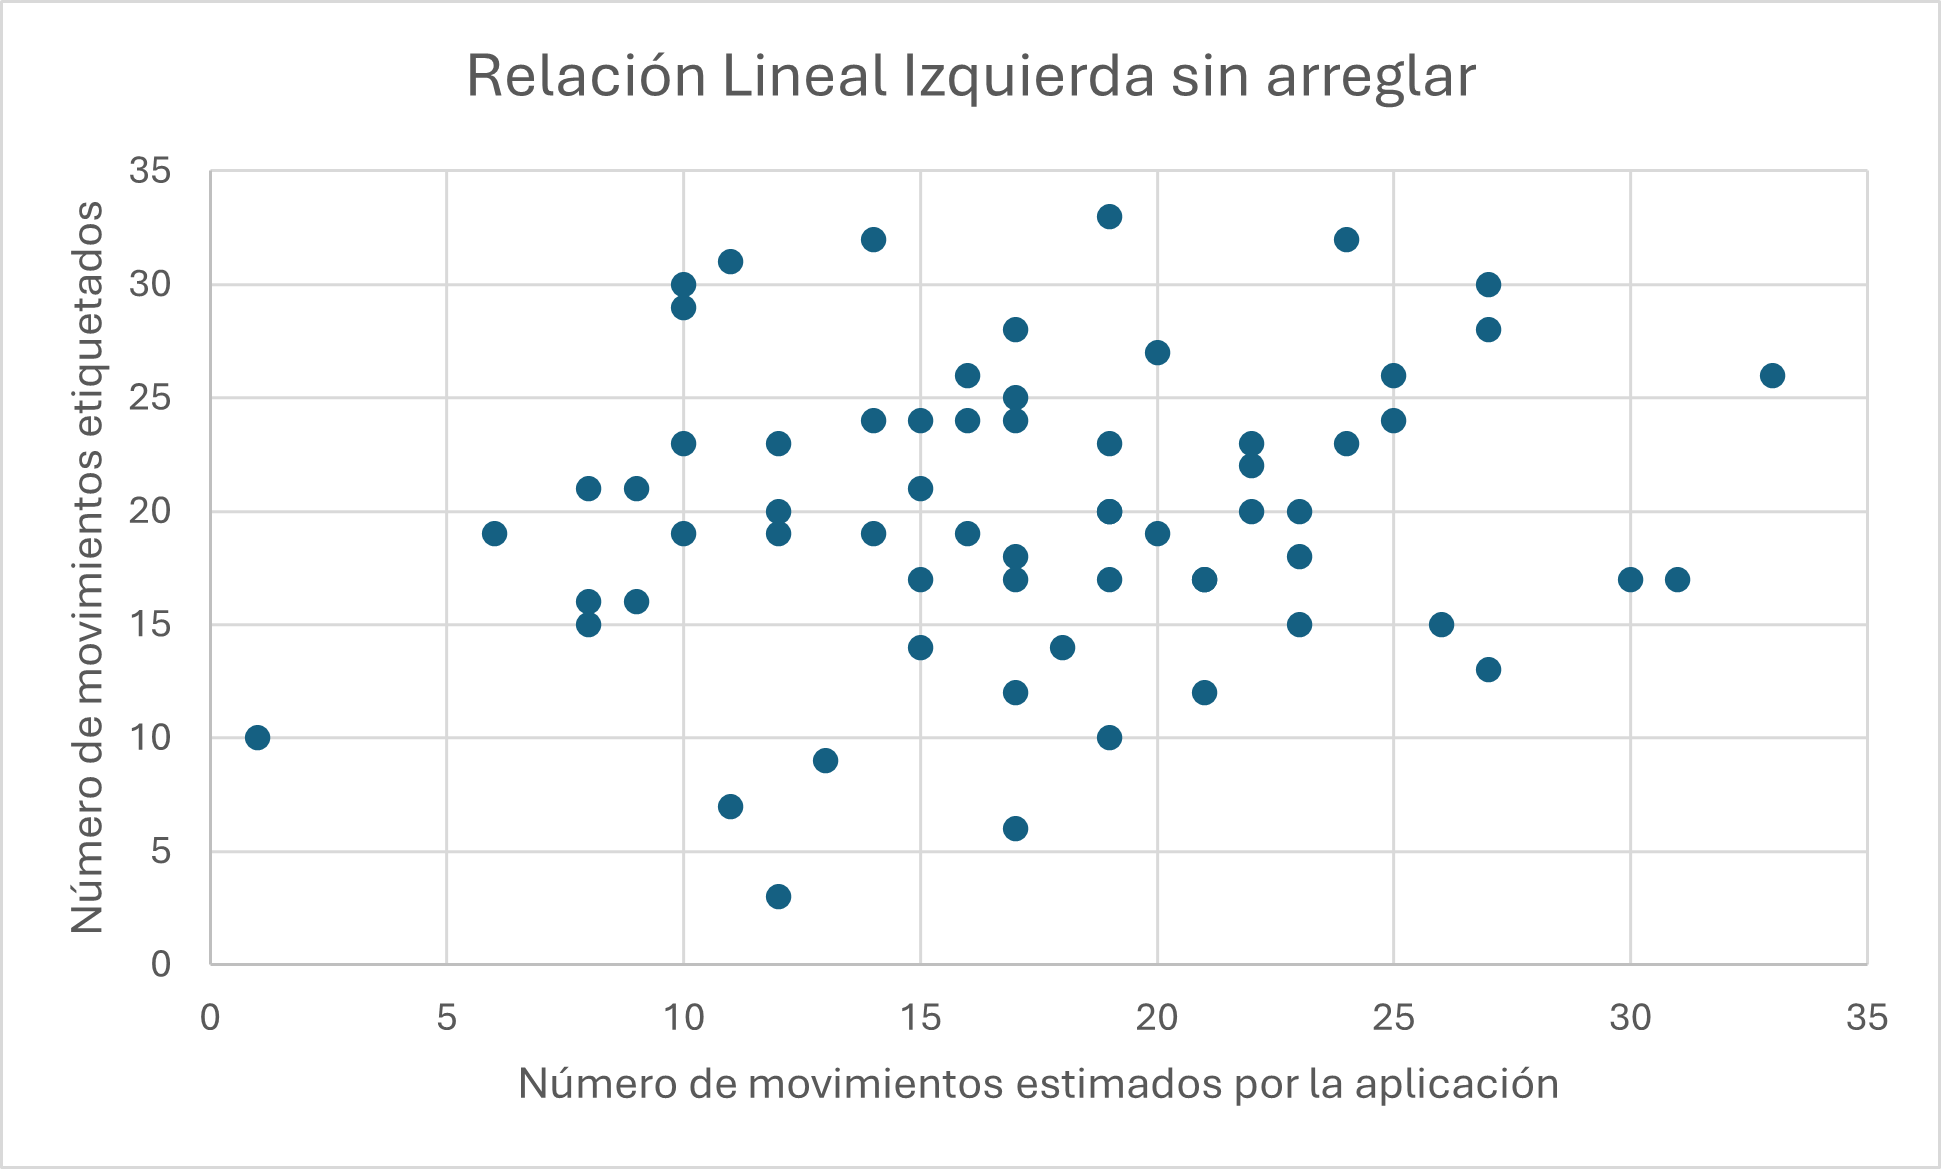
\includegraphics[width=0.9\textwidth]{images/7/IzquierdaMal.png}
        \caption{Relación lineal de los movimientos estimados y etiquetados en la izquierda sin el arreglo(Coeficiente R = 0,154365645)}
    \end{subfigure}
    \begin{subfigure}[b]{0.7\textwidth}
        \centering
        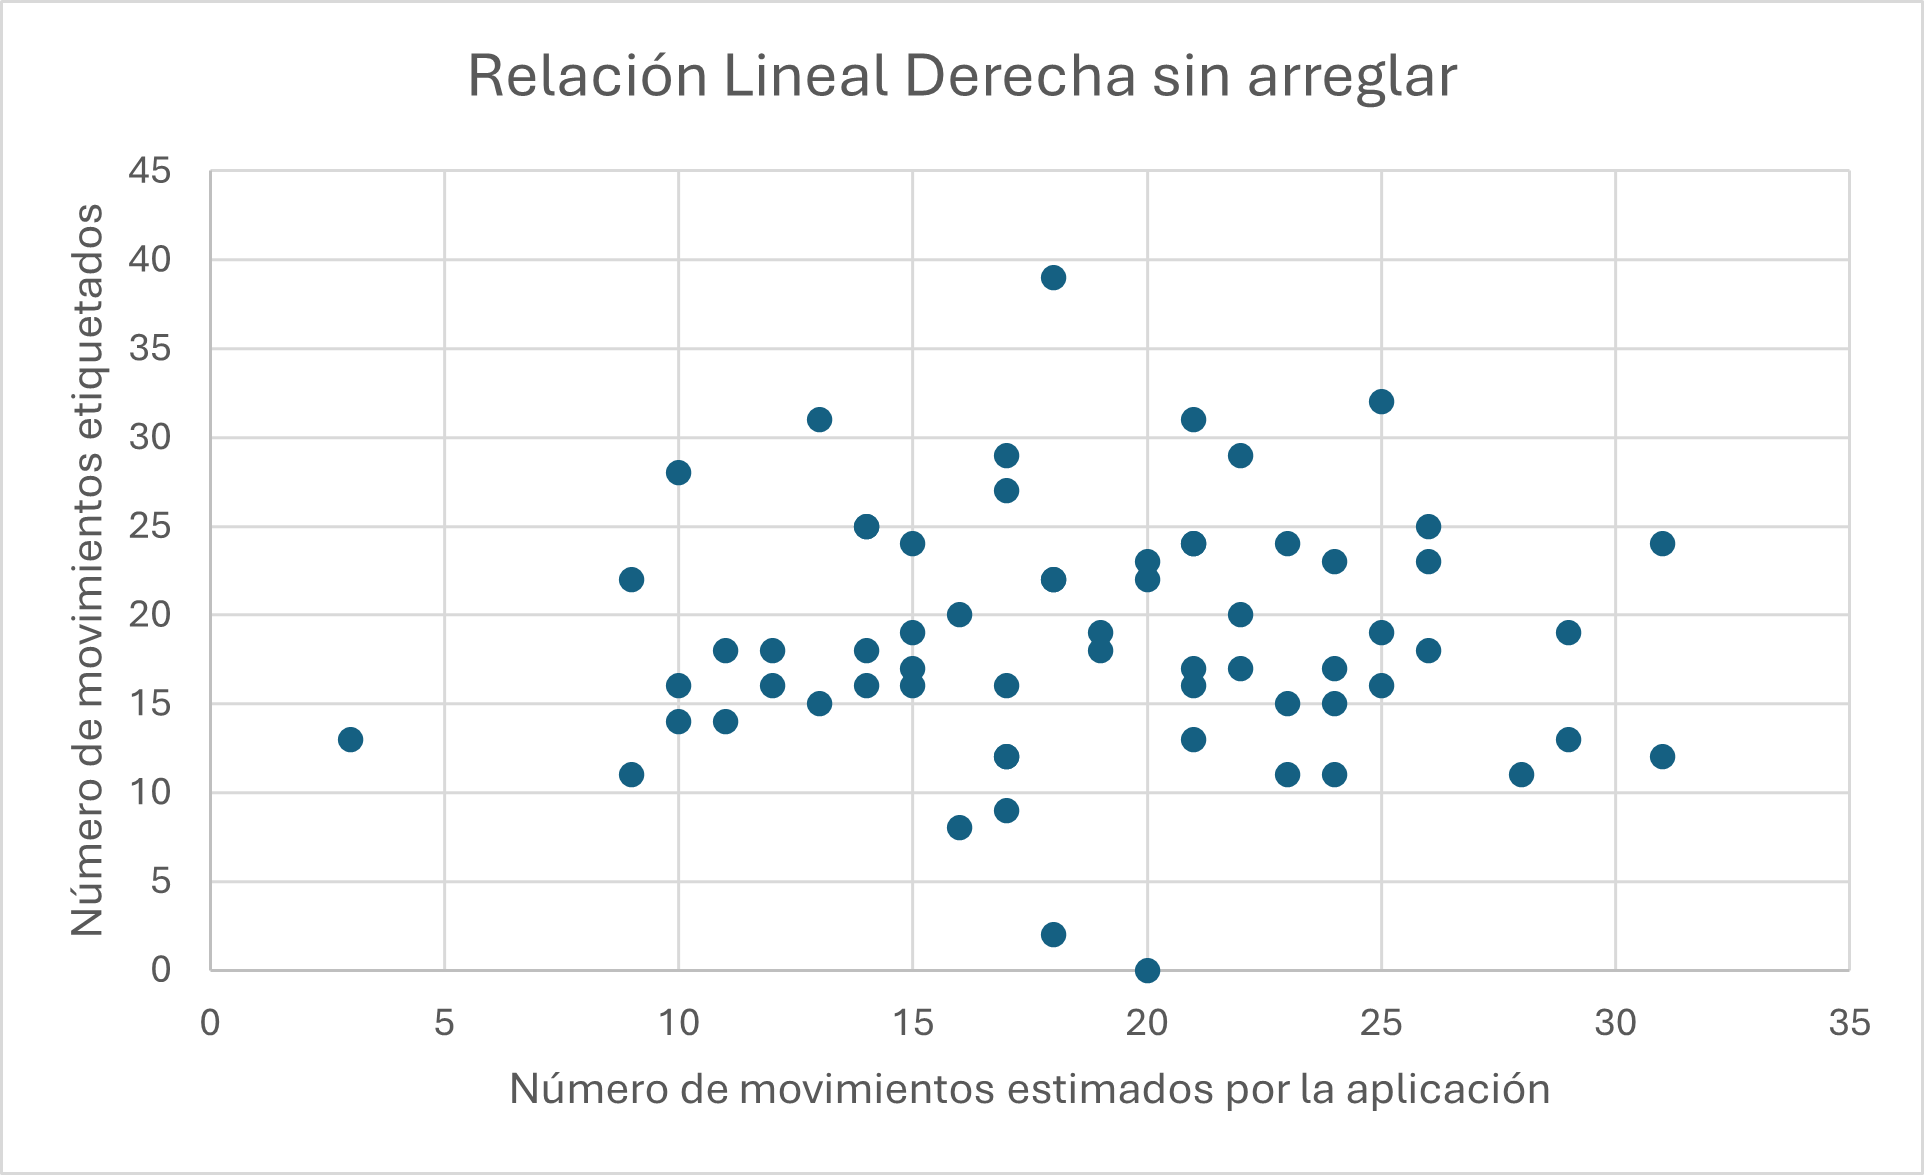
\includegraphics[width=0.9\textwidth]{images/7/DerechaMal.png}
        \caption{Relación lineal de los movimientos estimados y etiquetados en la derecha sin el arreglo(Coeficiente R = 0,032476833)}
    \end{subfigure}
    \caption{Relación de los datos estimados con los etiquetados asumiendo \texttt{LTR}}
    \label{fig:EtiquetadosMal}
\end{figure}

\begin{figure}[H]
    \centering
    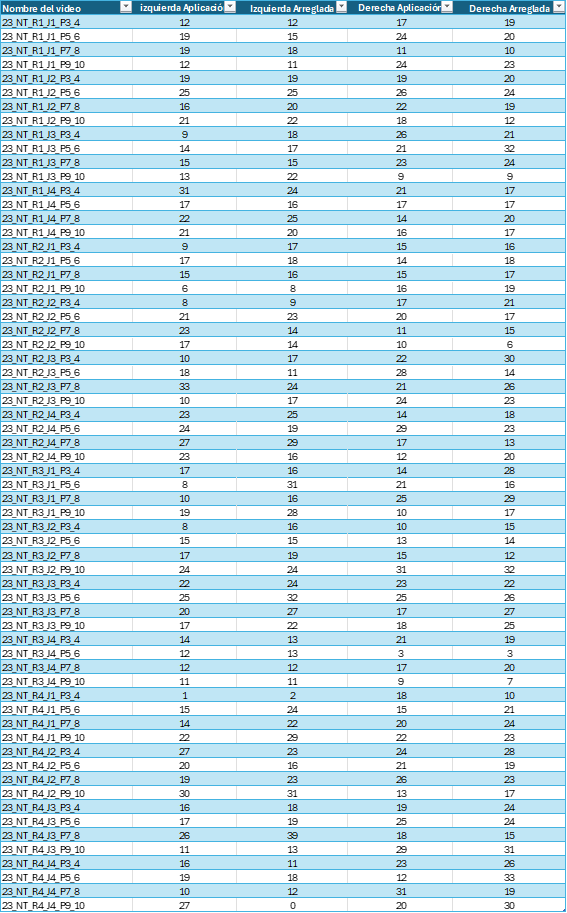
\includegraphics[width=0.85\textwidth]{images/7/ValidacionMovimientos.png}
    \caption{Tabla comparativa entre los movimientos estimados y los movimientos etiquetados}
    \label{fig:TablaResultados}
\end{figure}
\clearpage
Si se calcula según el arreglo de los datos, se obtienen las gráficas de la \autoref{fig:EtiquetadosBien}, donde se puede observar que la correlación de la aplicación y el algoritmo desarrollado es muy bueno para ser una primera versión.

\begin{figure}[H]
    \centering
    \begin{subfigure}[b]{0.7\textwidth}
        \centering
        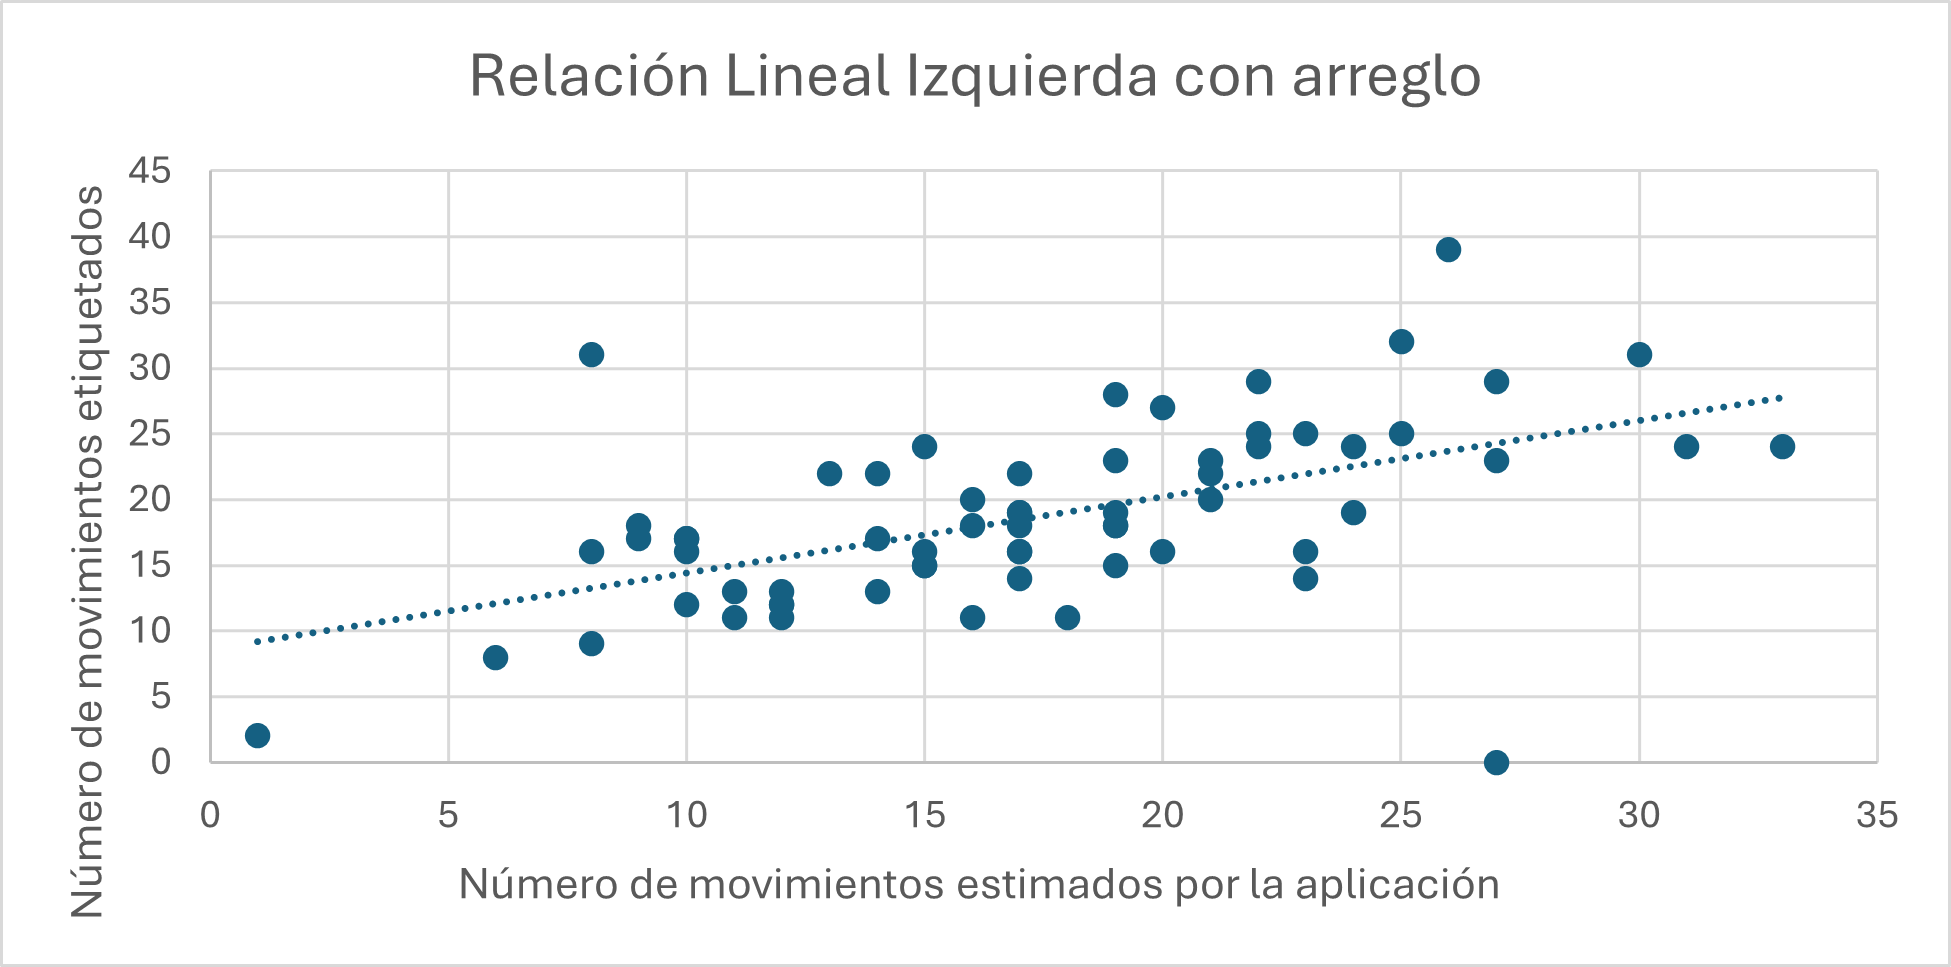
\includegraphics[width=0.9\textwidth]{images/7/IzquierdaBien.png}
        \caption{Relación lineal de los movimientos estimados y etiquetados en la izquierda con el arreglo(Coeficiente R = 0,539455863)}
    \end{subfigure}
    \begin{subfigure}[b]{0.7\textwidth}
        \centering
        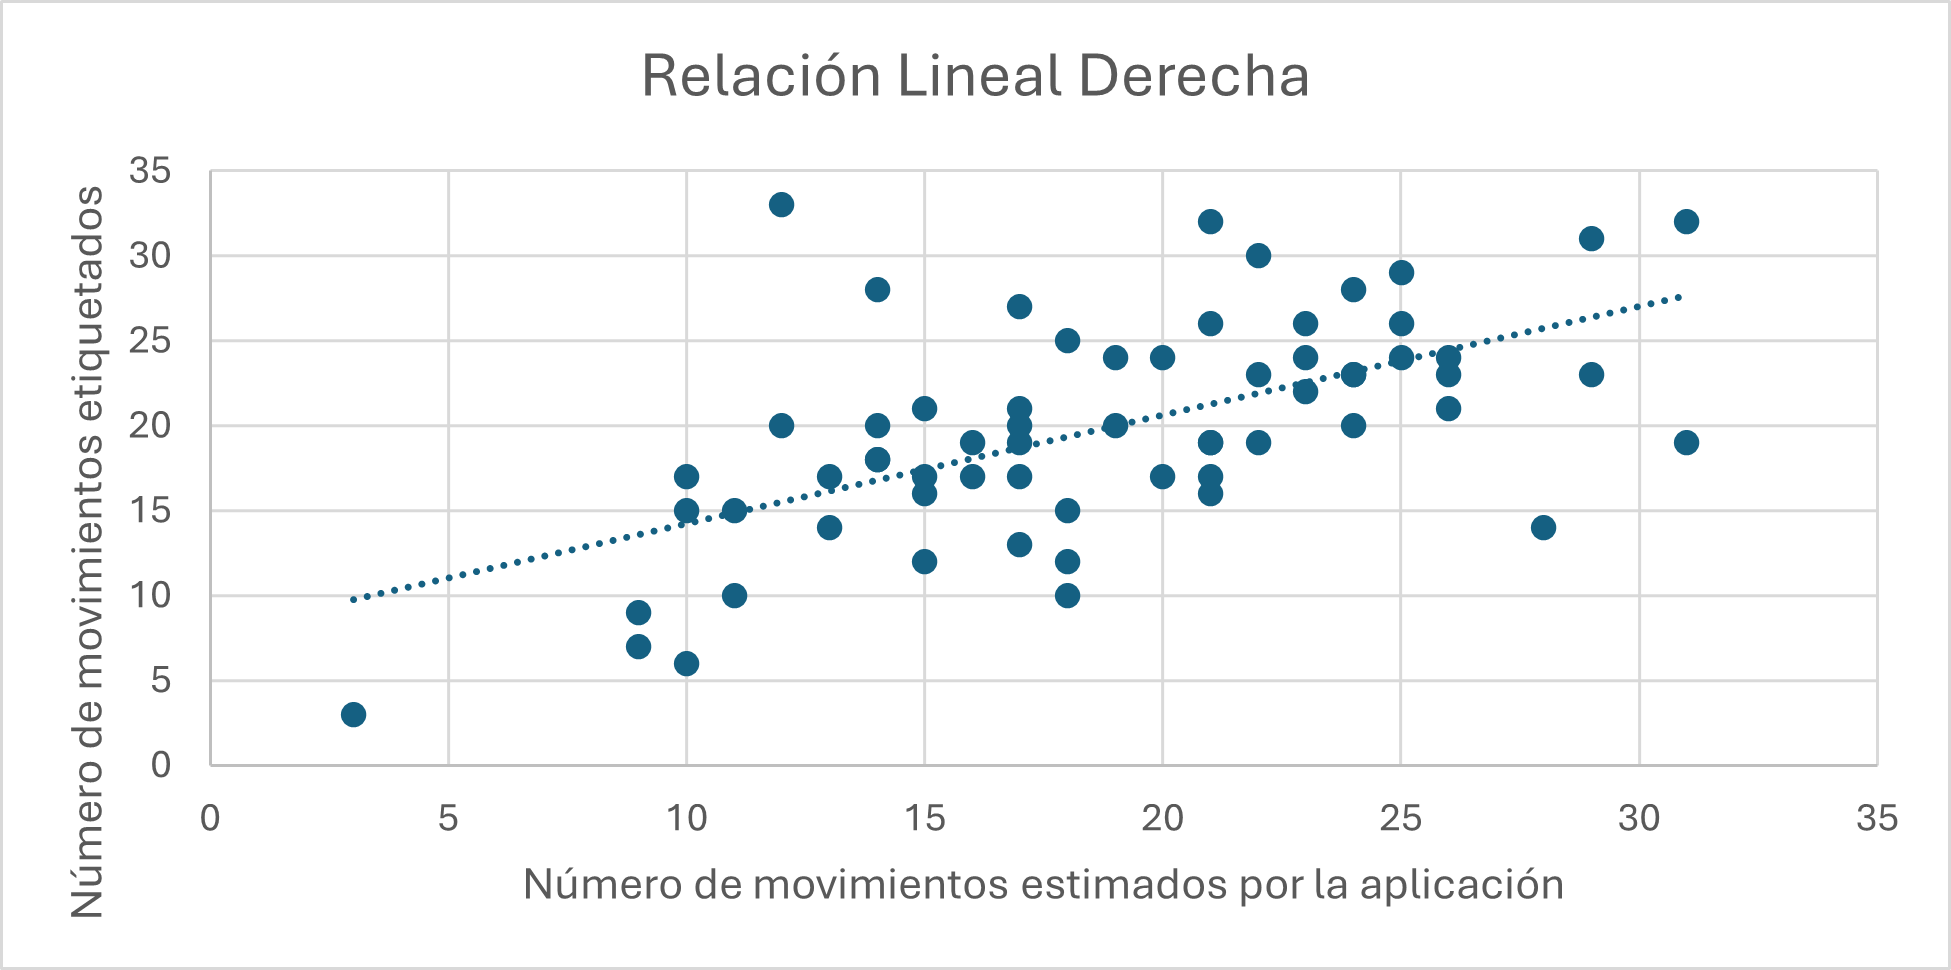
\includegraphics[width=0.9\textwidth]{images/7/DerechaBien.png}
        \caption{Relación lineal de los movimientos estimados y etiquetados en la derecha con el arreglo(Coeficiente R = 0,584222239)}
    \end{subfigure}
    \caption{Relación de los datos estimados con los etiquetados aplicando el arreglo}
    \label{fig:EtiquetadosBien}
\end{figure}
\vspace{3\baselineskip}
Finalmente, se ha calculado los respectivos histogramas de la \autoref{fig:HistogramasError}, en donde se puede observar la distribución del error en la validación. Se puede observar que la mayor parte del error está entre -20\% y el 30\%.

\begin{figure}[H]
    \centering
    \begin{subfigure}[b]{0.7\textwidth}
        \centering
        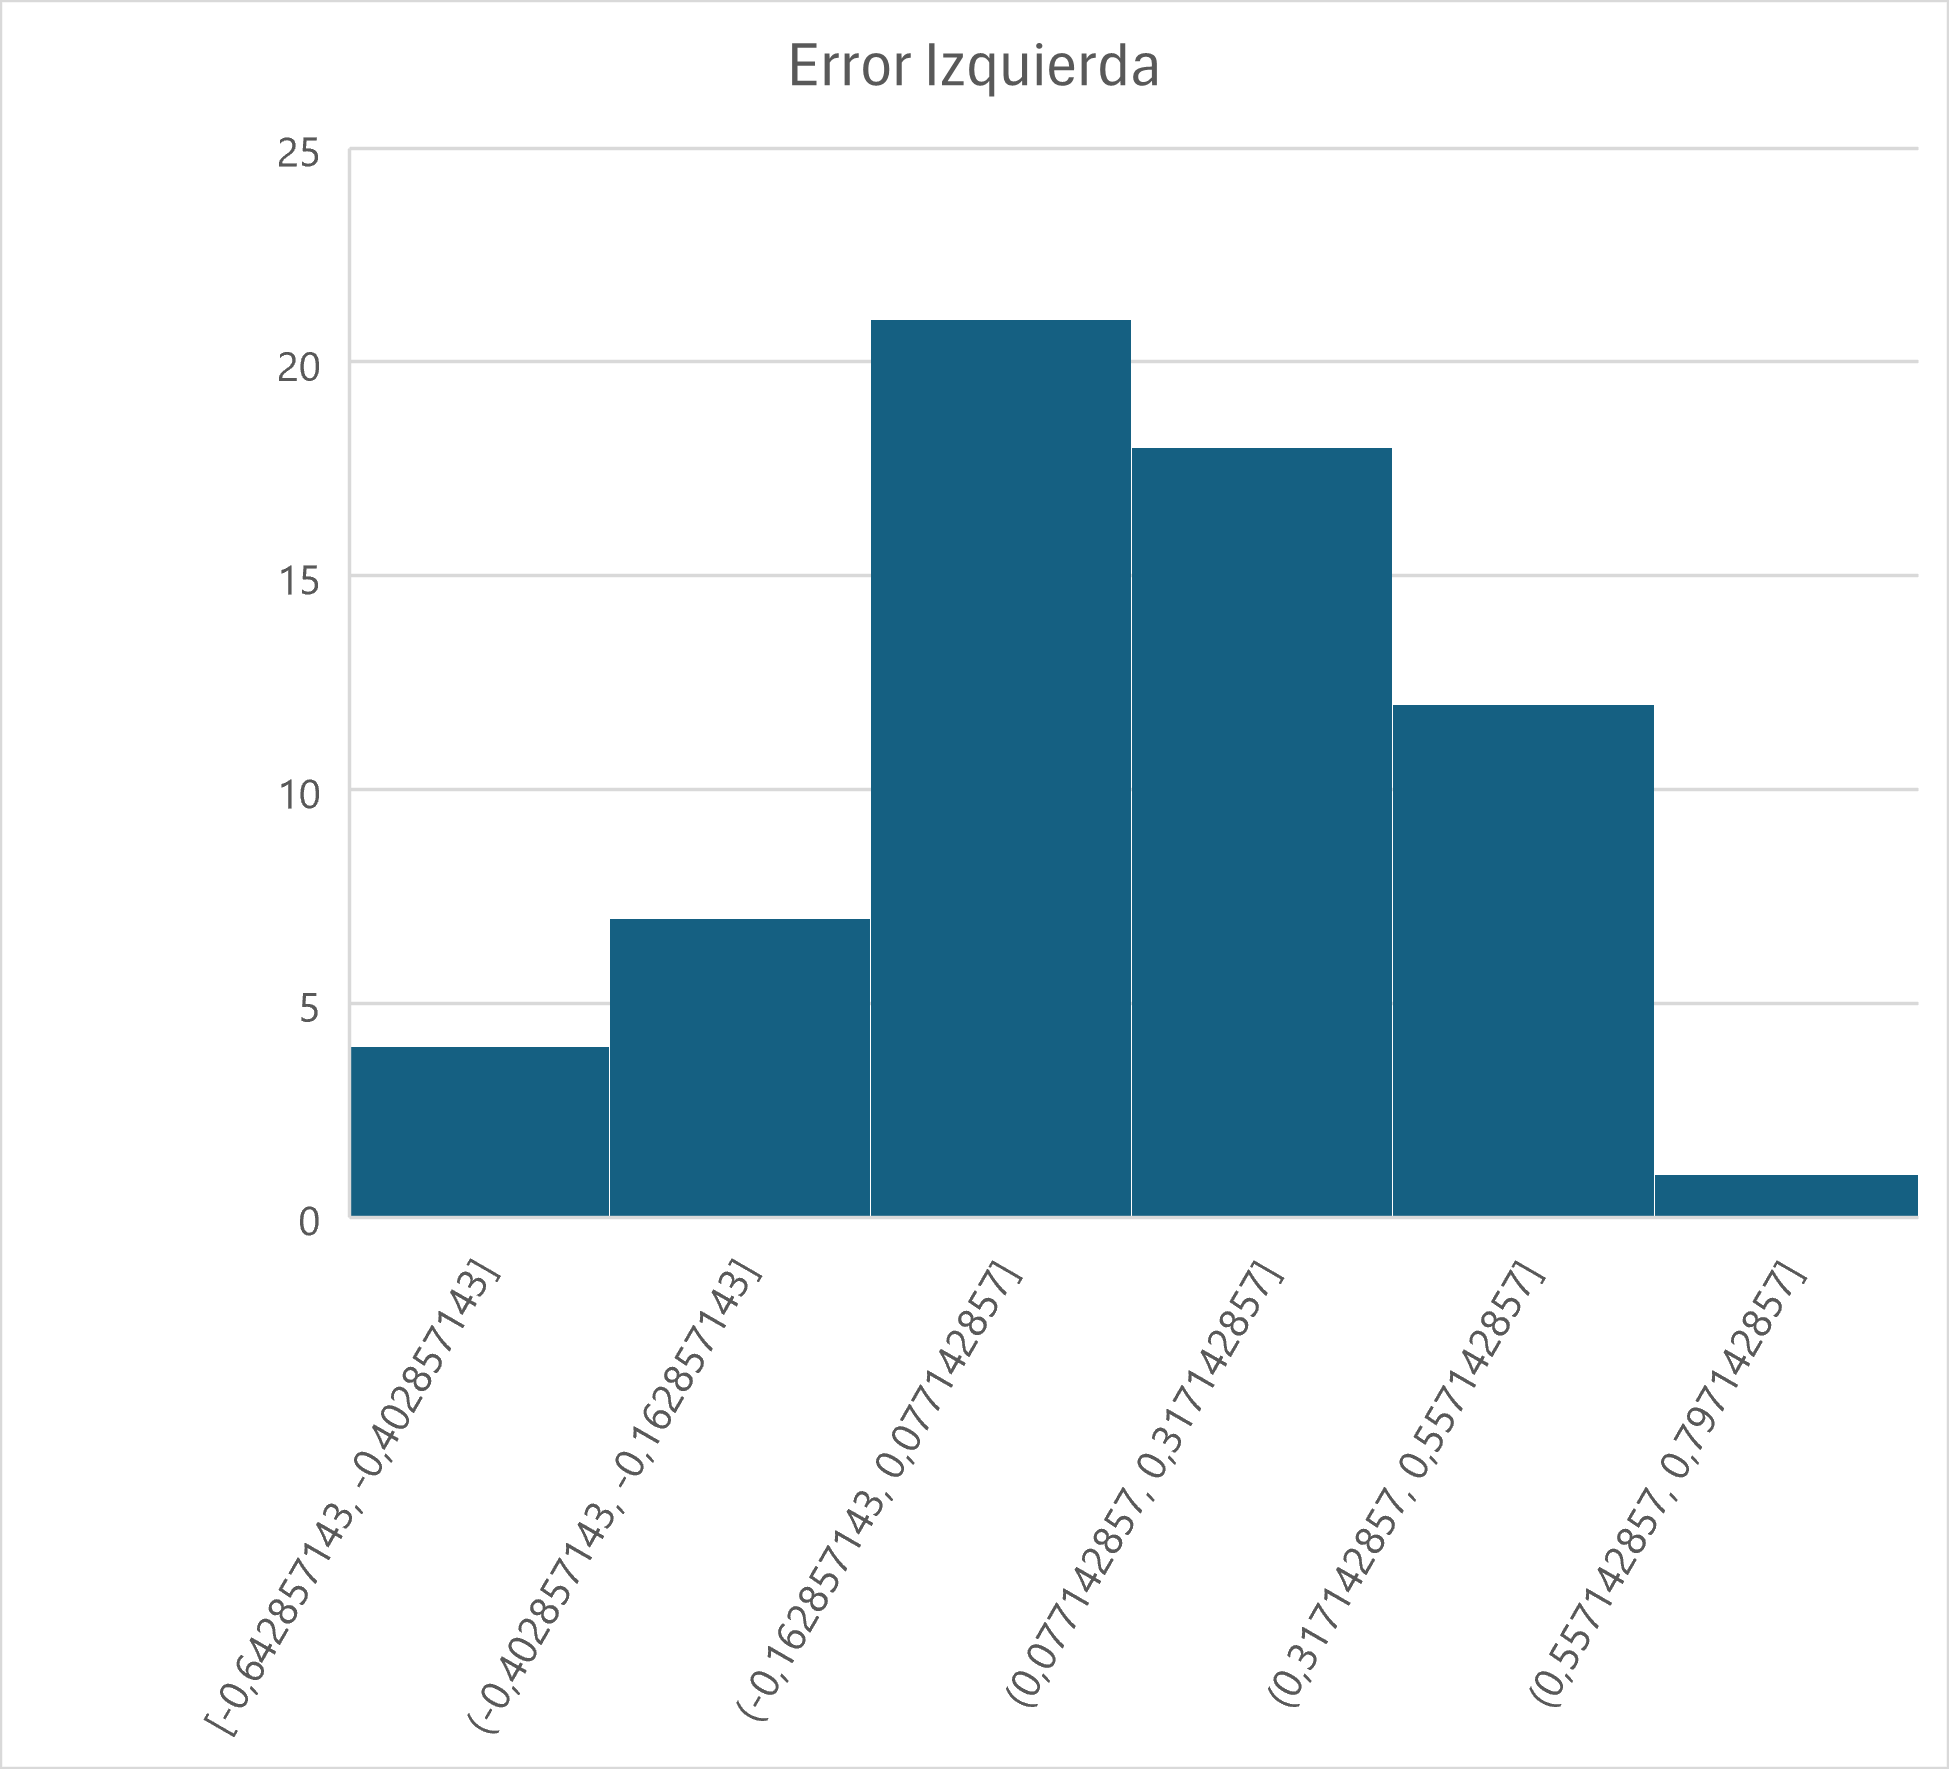
\includegraphics[width=0.9\textwidth]{images/7/ErrorIzquierda.png}
        \caption{Distribución del error en las truchas de la izquierda en validación de resultados}
    \end{subfigure}
    \begin{subfigure}[b]{0.7\textwidth}
        \centering
        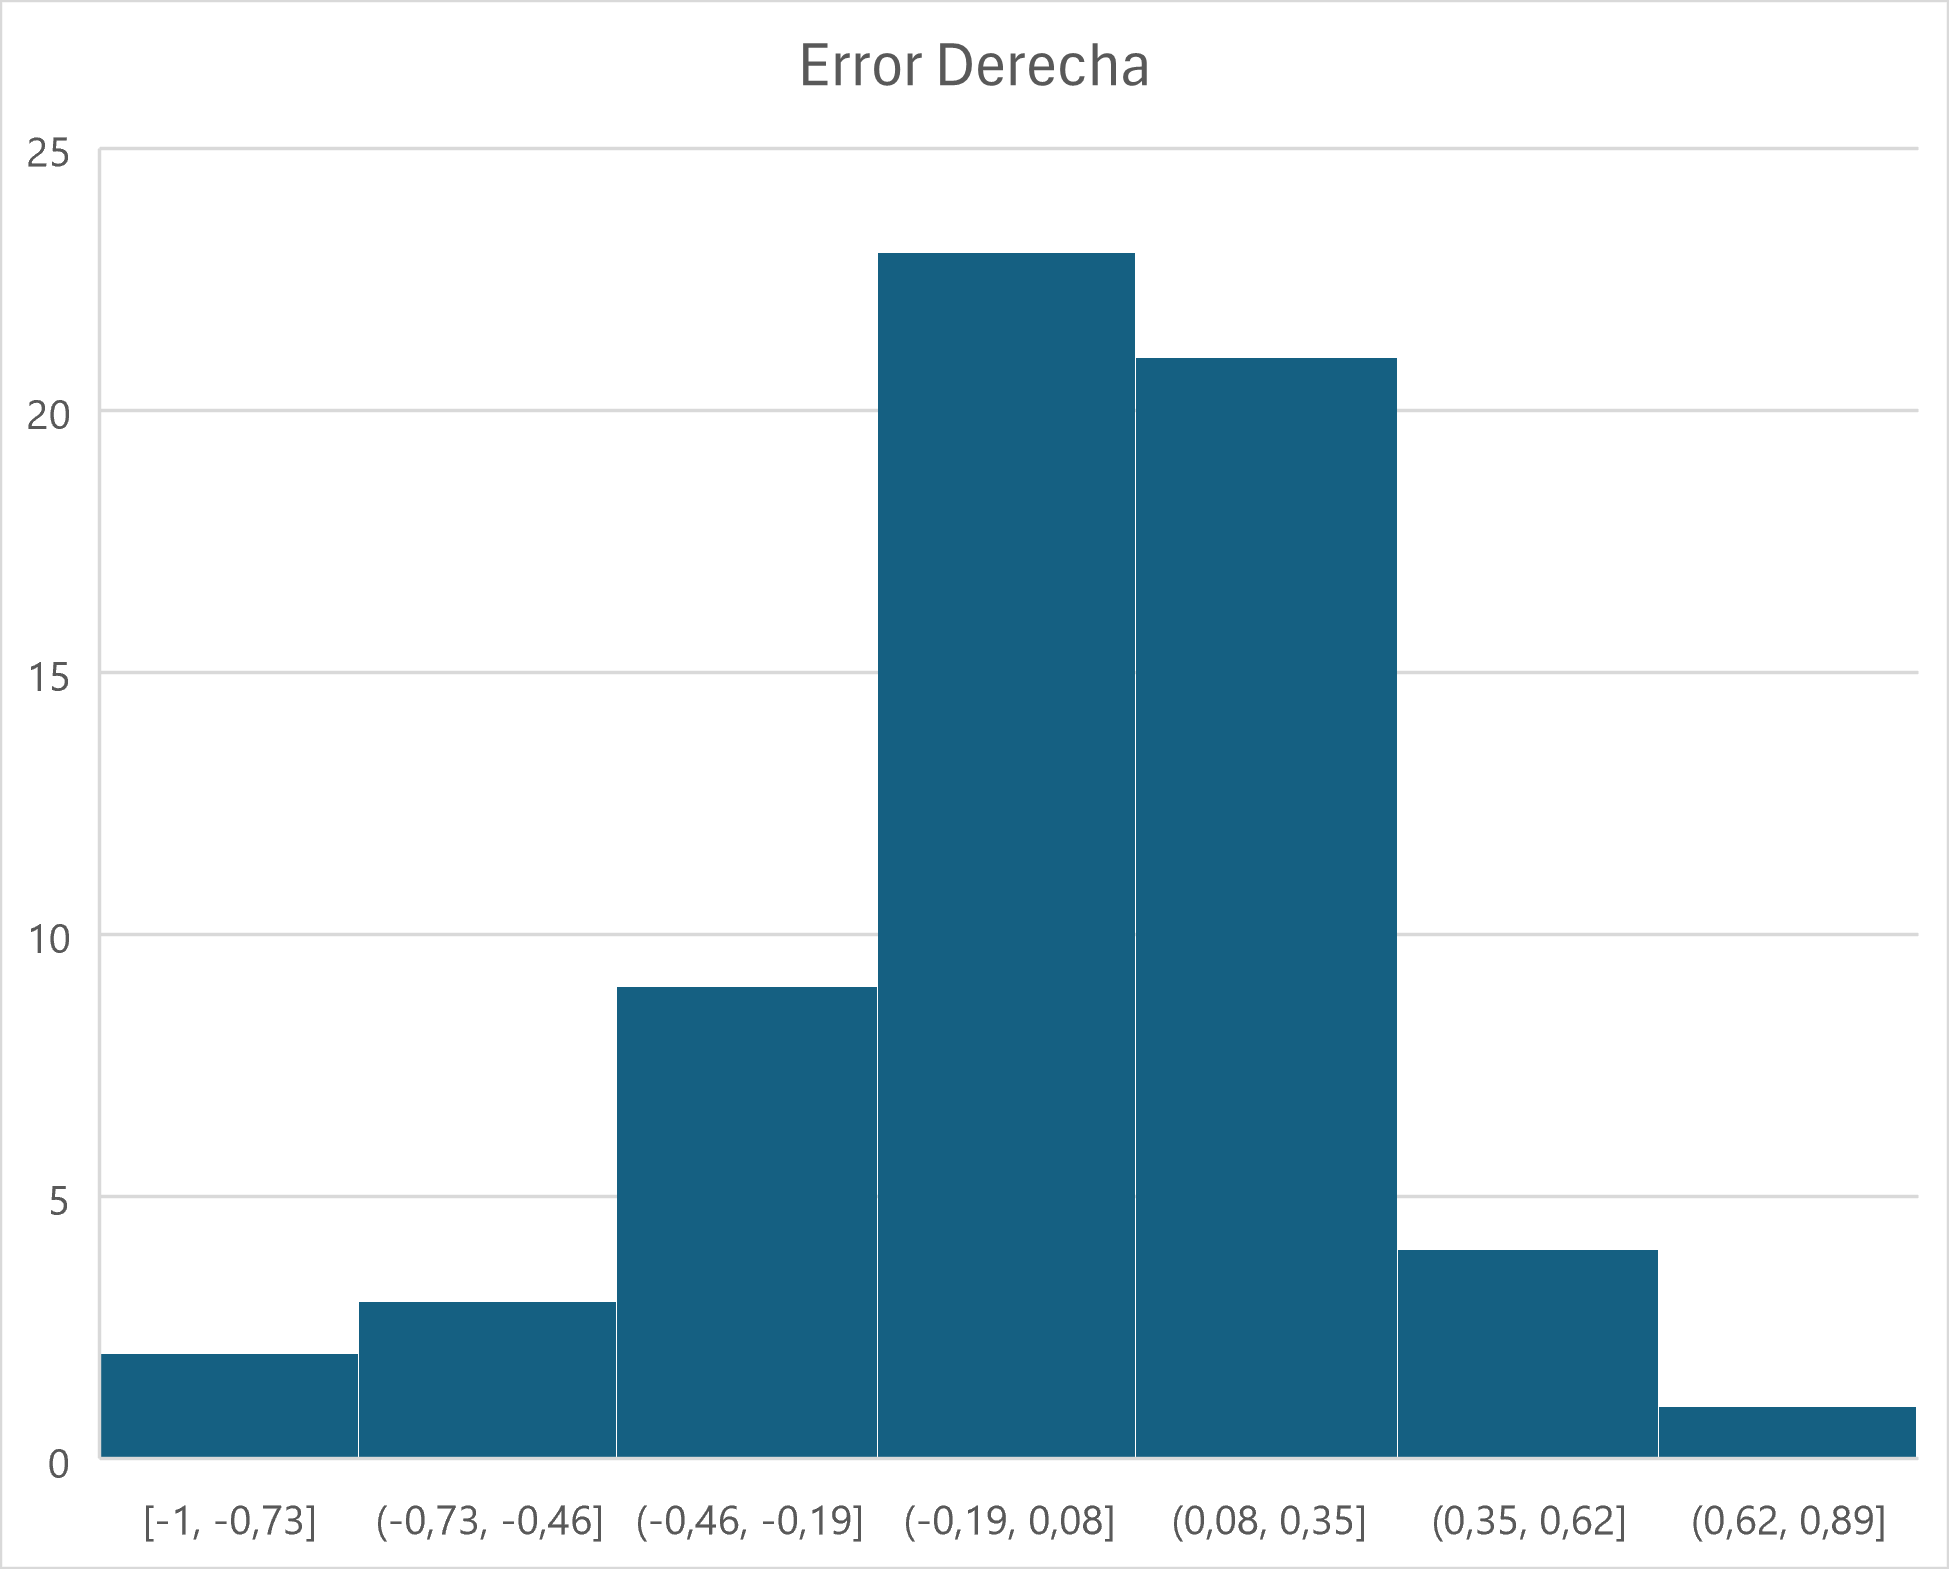
\includegraphics[width=0.9\textwidth]{images/7/ErrorDerecha.png}
        \caption{Distribución del error en las truchas de la derecha en validación de resultados}
    \end{subfigure}
    \caption{Distribución del error respecto a las etiquetas de los investigadores}
    \label{fig:HistogramasError}
\end{figure}

Como resumen, la detección y el conteo de movimiento se ha hecho correctamente, si bien hay errores que pueden provenir de diversos factores como la subjetividad del etiquetado manual y falta de ajuste del algoritmo de conteo 
de movimientos de la aplicación. Sin embargo, como primera aproximación al problema permite ver fácilmente el comportamiento de las truchas de manera comparativa en el \textit{NetTest}.

\clearpage

La última validación de resultados que falta es la relacionada con el rendimiento de la aplicación y el uso del \texttt{HardWare}. En este sentido:

\begin{itemize}
    \item Se ha conseguido una aplicación que consigue seleccionar el mejor formato de red neuronal según el ordenador en el que se ejecute, permitiendo minimizar el tiempo necesario para procesar un video. Esto se ve reflejado en 
    los anteriores resultados, en los que se han procesado 64 videos de 15 segundos cada uno en solo 1 hora en total.
    \item A través de \texttt{DearPyGUI}, se consigue una aplicación fluida que mantiene una tasa de fotogramas sin caídas, lo que provee una experiencia muy buena al usuario.
    \item A través del uso de procesos, se ha conseguido descargar el hilo principal, minimizar tiempos de proceso e implementar funciones multimedia sin que afecte al rendimiento. Esto se ve reflejado en la carga que tiene la 
    aplicación sobre la memoria \texttt{RAM}, que en las pruebas no ha superado el umbral de \texttt{1.5GB} en ningún momento para videos de resolución \texttt{1080P}.
\end{itemize}

\section{PRESUPUESTO}

En este apartado se describen los costes de desarrollo que conlleva este trabajo, detallándose el coste de los recursos de forma individual. Estos pueden ser materiales, mano de obra u otros.

En el proyecto ha habido 4 fases:
\begin{enumerate}
    \item Estudio y análisis del estado del arte (45h)
    \item Pruebas de diseño y concepto (85h)
    \item Implementación de la solución (160h)
    \item Documentación del trabajo (60h)
\end{enumerate}

El punto 1 y 2 se han considerado investigación, siendo el punto 3 y 4 partes de la fase de desarrollo.

En la \autoref{presupuestoGeneral} se presenta el presupuesto general:

\begin{table}[H]
    \begin{tabular}{|lll|l|}
    \hline
    \multicolumn{1}{|l|}{\textit{\textbf{Nombre}}} & \multicolumn{1}{l|}{\textit{\textbf{Precio unitario (€)}}} & \textit{\textbf{Unidades}} & \textit{\textbf{Precio total(€)}} \\ \hline
    \multicolumn{1}{|l|}{Personal de investigación}            & \multicolumn{1}{l|}{20}      & 130  & 2400               \\ \hline
    \multicolumn{1}{|l|}{Personal de desarrollo}               & \multicolumn{1}{l|}{20}      & 220  & 4400               \\ \hline
    \multicolumn{1}{|l|}{Ordenador portátil Asus F1704VA}      & \multicolumn{1}{l|}{150}     & 1    & 150                \\ \hline
    \multicolumn{1}{|l|}{Torre MSI}                            & \multicolumn{1}{l|}{30}      & 1    & 30                 \\ \hline
    \multicolumn{1}{|l|}{Equipo NAS para los videos}           & \multicolumn{1}{l|}{50}      & 1    & 50                 \\ \hline
    \multicolumn{3}{|r|}{\textbf{Total=}}                                                            & 7030               \\ \hline
    \end{tabular}
    \caption{Presupuesto general del proyecto}
    \label{presupuestoGeneral}
\end{table}

En este caso, algunos de los equipos ya habían sido proporcionados previamente, por lo tanto se aplicó una amortización respecto al valor del producto:
\begin{itemize}
    \item Ordenador portátil Asus F1704VA (Valor original: 600€) amortización de 150€.
    \item Torre MSI (Valor original: 1000€) amortización de 30€.
    \item Equipo NAS (Valor original: 1200€) amortización de 50€.
\end{itemize}

Por como se ha planteado el proyecto, los programas usados durante el desarrollo son de libre uso o gratis, por lo tanto no ha sido necesario incluirlos en el presupuesto.
\newpage
\thispagestyle{abstract}
\mbox{}
\newpage
\section{MANUAL DE USUARIO}
\section{ANÁLISIS DE IMPACTO DEL PROYECTO}

Como se discutió en la introducción de este trabajo, el cambio climático cada vez está tomando más importancia en la sociedad. Dentro de todas las herramientas que existen para reducir su 
efecto, está la investigación para la reducción de huella de carbono en la generación de alimento. Especialmente, se están realizando muchas investigaciones con la acuicultura, ya que es un 
método muy seguro y controlado para cubrir las necesidades de proteína de origen marítimo y evitar la perdida de los ecosistemas marítimos.

Este trabajo tiene un impacto social, siendo este no sobre el ser humano, sino sobre los animales. La herramienta que se ha generado permite a investigadores parametrizar de forma experimental 
las consecuencias que tiene un tratamiento u otro. Esto tiene como objetivo determinar técnicas que aumenten el bienestar animal en las piscifactorías.

En el análisis de impacto económico, este trabajo mejora sistemas que antes tomarían demasiado tiempo y serían propensos a errores humanos, lo cual se transforma en una reducción del dinero 
perdido en analizar recursos como videos.

Dentro del análisis de impacto también aparece la eliminación de la brecha digital a la hora de gestionar resultados de experimentos con áreas que no son la ingeniería.

\subsubsection*{Objetivos de Desarrollo Sostenible}

Este trabajo busca alinearse con los \acrshort{ods} definidos por la Unión Europea. Dentro de los objetivos individuales que se ven afectados por este trabajo tenemos:
\begin{itemize}
    \item \textbf{Trabajo decente y crecimiento económico}: los investigadores que pierden más tiempo analizando videos que realizando experimentos y obteniendo conclusiones van a ver esta herramienta 
    para automatizar procesos llenos de errores humanos.
    \item \textbf{Industria, innovación e infraestructura}: este trabajo busca dar herramientas para mejorar las condiciones animales en la industria de la acuicultura.
    \item \textbf{Producción y consumo responsables}: si se mejora la calidad animal en la acuicultura, la producción aumentara y será menos necesario utilizar los entornos marítimos para realizar pesca 
    masiva.
    \item \textbf{Acción por el clima}: mejorar las condiciones de producción en la acuicultura reduce los beneficios que produce la pesca de alta mar.
    \item \textbf{Vida submarina}: la obtención de proteína a través de la acuicultura consigue aliviar los entornos marinos.
\end{itemize}
\newpage
\thispagestyle{abstract}
\mbox{}
\newpage
\section{CONCLUSIONES Y TRABAJOS FUTUROS}

Los experimentos actuales en la ciencia cada vez manejan mayores cantidades de datos. La capacidad de automatizar la obtención de los datos, su procesado y su análisis es uno de los campos más importantes 
de la tecnología moderna. Dentro de esto encontramos la visión por ordenador como campo que engloba diversas tecnologías para procesar imagen.

Dentro la visión por ordenador, uno de los paradigmas más eficientes en la actualidad para conseguir analizar videos son las arquitecturas de redes neuronales \texttt{CNN}l que aprovechan un planteamiento de 
operaciones por matrices para poder manejar grandes cantidades de datos a la vez. Una de las \texttt{CNN} más populares actualmente es \texttt{YOLOv8} por su rendimiento y eficiencia.

A través de pruebas comparativas, se ha observado que respecto a métodos tradicionales como el análisis de flujo óptico, las arquitecturas \texttt{CNN}; más específicamente \texttt{YOLO}, se pueden usar 
para caracterizar el movimiento de truchas de forma extremadamente rápida. Estos sistemas son capaces de reconocer correctamente truchas en movimiento y con una tasa de error muy baja con poco tiempo de entrenamiento.

En este trabajo se ha usado el modelo \texttt{YOLO} entrenado para la detección de truchas para construir una aplicación que cuente el número de movimientos. Para conseguir esto se han aprovechado técnicas como 
los sistemas basados en ejecución paralela y la correcta elección del modelo dependiendo del \texttt{HardWWare} disponible del ordenador. Con esto se han conseguido obtener resultados como el 
procesamiento de 64 videos en 1 hora, obteniendo una tasa de error respecto a los movimientos detectados sobre movimientos previamente etiquetados en su mayoría de entre -20\% y 20\%. \newline
Estos resultados son muy buenos y cumplen con los objetivos marcados en el proyecto.

Con todo esto se ha conseguido construir una aplicación capaz de funcionar a tiempo real, que no necesita conocimientos de tecnologías sobre las redes neuronales, lenguajes de programación o 
uso de una consola de comandos para ser usada. Esto permite potenciar la automatización de procesos experimentales en campos donde el uso de este tipo de herramientas va retrasado.

A través de este trabajo, se ha podido estudiar el desarrollo de soluciones aplicando técnicas de ingeniería (Planteamiento → Prueba de concepto → Desarrollo → Validación de resultados → Entrega final), entendiendo 
los requisitos que puede tener una persona ajena al mundo de la ingeniería y sabiendo definir las limitaciones que puede tener la puesta a prueba de un concepto en un entorno real donde hay variables que no se 
pueden controlar.

\vspace{2\baselineskip}

Las futuras líneas que se plantean en este trabajo son las siguientes:
\begin{itemize}
    \item Mejora de la interfaz de usuario: principalmente añadir funcionalidades centradas en la accesibilidad.
    \item Mejora de la red neuronal: hacer un \texttt{fine-tunning} de hiperparámetros y realizar un entrenamiento lo mejor posible teniendo un conjunto de datos mucho más amplio. Esto permitiría ajustar completamente la 
    \texttt{Bounding Box} de la trucha. También sería interesante entrenar la red neuronal para trabajar con peces similares.
    \item Despliegue sobre dispositivos IoT y creación de un cliente ligero: esto permitiría distribuir el sistema y que un usuario pudiese usarlo sin tener un ordenador de altas prestaciones.
    \item Mejorar el algoritmo de control de movimiento: plantear una alternativa mucho más flexible e inteligente, como un árbol de decisión.
\end{itemize}
\newpage
\thispagestyle{abstract}
\mbox{}
\newpage
\clearpage
\nocite{*} % Aunque no cites x, se mete en la bibliografía, * es todo de
\printbibliography[title={BIBLIOGRAFÍA}, heading=bibnumbered]
\newpage
\thispagestyle{abstract}
\mbox{}
\newpage
\clearpage
\section{ANEXOS}
\subsection*{ANEXO A: Explicación de los hiperparámetros y resultados de YOLO}
\label{subsec:A}

Las redes neuronales como \texttt{YOLO} y en general todas las que utilizan entrenamiento supervisado, tienen como objetivo acercarse lo máximo posible al resultado esperado en las etiquetas de entrenamiento. 
A lo largo de este entrenamiento se van actualizando parámetros (valores que sí cambian en entrenamiento) como son los pesos, los \texttt{bias} y otros elementos. Esta búsqueda de aproximación se puede ver 
reflejada como la búsqueda de mínimos globales en una función, en la mayoría de casos es buscar los mínimos globales de la función de perdidas. Esto se puede ver en la \autoref{fig:GradientDescendGlobales}.

\begin{figure}[H]
    \centering
    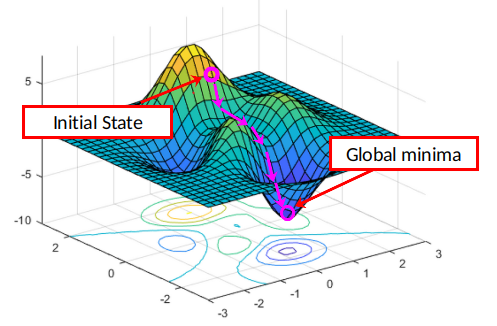
\includegraphics[width=0.5\textwidth]{images/13/a/GradientDescend.png}
    \caption{Búsqueda de mínimos globales por un algoritmo de aprendizaje automático\cite{doleronDeepLearningScratch2023}}
    \label{fig:GradientDescendGlobales}
\end{figure}

Los modelos de \texttt{YOLO} tienen definidos una serie de hiperparámetros (valores que no cambian en entrenamiento) que sirven como ajustes fijos durante en el entrenamiento. 
Estos hiperparámetros ajustan la manera en la que el algoritmo decide el siguiente paso a tomar en su búsqueda de un mínimo global y pueden acelerar o ralentizar el tiempo necesario 
de entrenamiento para alcanzar unos valores de perdida adecuados. Algunos de los hiperparámetros más típicos\cite{ultralyticsConfiguration} son:

\begin{itemize}
    \item \textbf{Learning Rate inicial}: es el valor que afecta cuanto se cambian los pesos entre época. Por defecto es \texttt{0.01}, que puede parecer poco, pero es mejor dar pasos pequeños para llegar al mínimo global.
    \item \textbf{Learning Rate final}: es una fracción del valor inicial. Según se realiza el entrenamiento de la red es normal reducir el \texttt{Learning Rate} para ajustar de forma más fina. Por defecto es \texttt{0.01}.
    \item \textbf{Momentum}: es una variable que permite tener en cuenta que camino se ha recorrido en la anterior época, para no volver a situaciones anteriores y seguir progresando. Por defecto es \texttt{0.937}.
    \item \textbf{Weight Decay}: hiperparámetro para prevenir sobreajuste y penalizar los pesos que son extremadamente grandes en la red.
    \item \textbf{Épocas de calentamiento}: número de épocas que se utilizaran para ir poco a poco acercándose a los valores iniciales de \texttt{Learning Rate}. Por defecto su valor es 3.
    \item \textbf{Tamaño de lote}: número de imágenes que se utilizaran en una pasada. Si tenemos 50 imágenes y el tamaño del lote es 10, se pasaran 10 y se ajustaran los pesos, y en este caso una época se compondra 
    de 5 pasadas de lote.
    \item \textbf{Número de épocas}
    \item \textbf{Número de capas ocultas}
\end{itemize}
\clearpage
Además, \texttt{YOLO} utiliza de base una herramienta de aumento de datos simple, por lo tanto tenemos muchos hiperparámetros para ajustar su funcionamiento:

\begin{itemize}
    \item \textbf{Hsv componente h}: ajusta el \texttt{Hue} de la imagen por una fracción que por defecto es \texttt{0.015}.
    \item \textbf{Hsv componente s}: ajusta la saturación de la imagen por una fracción que por defecto es \texttt{0.7}, permite simular diferentes condiciones de iluminación.
    \item \textbf{Hsv componente v}: modifica el brilo de la imagen, por defecto a una fracción de \texttt{0.4}.
    \item \textbf{Translate}: mueve la imagen horizontal y verticalmente por defecto un \texttt{10\%}.
    \item \textbf{Scale}: ajusta el tamaño de la imagen para simular diferentes distancias a la cámara. Por defecto \texttt{0.5}.
    \item \textbf{Fliplr}: espeja la imagen horizontalmente con una probabilidad por defecto de \texttt{0.5}.
    \item \textbf{Mosaic}: permite combinar 4 imágenes en una para crear imágenes compuestas que mejoran mucho la calidad del entrenamiento. Por defecto siempre está activo.
    \item \textbf{Erasing}: borra partes de la imagen de forma aleatoria para que el modelo sepa reconocer segmentos del elemento y que sea capaz de detectar características más específicas.
    \item \textbf{Crop fraction}: de forma aleatoria corta la imagen a fracciones de su tamaño original.
\end{itemize}
El resultado de este aumento de datos se puede ver en los lotes con los que se entrena la red como el de la \autoref{fig:AumentoDatosYolo}, donde vemos cambios de brillo, saturación, recortes de imagen y 
combinación de imágenes en diferentes tamaños.
\begin{figure}[H]
    \centering
    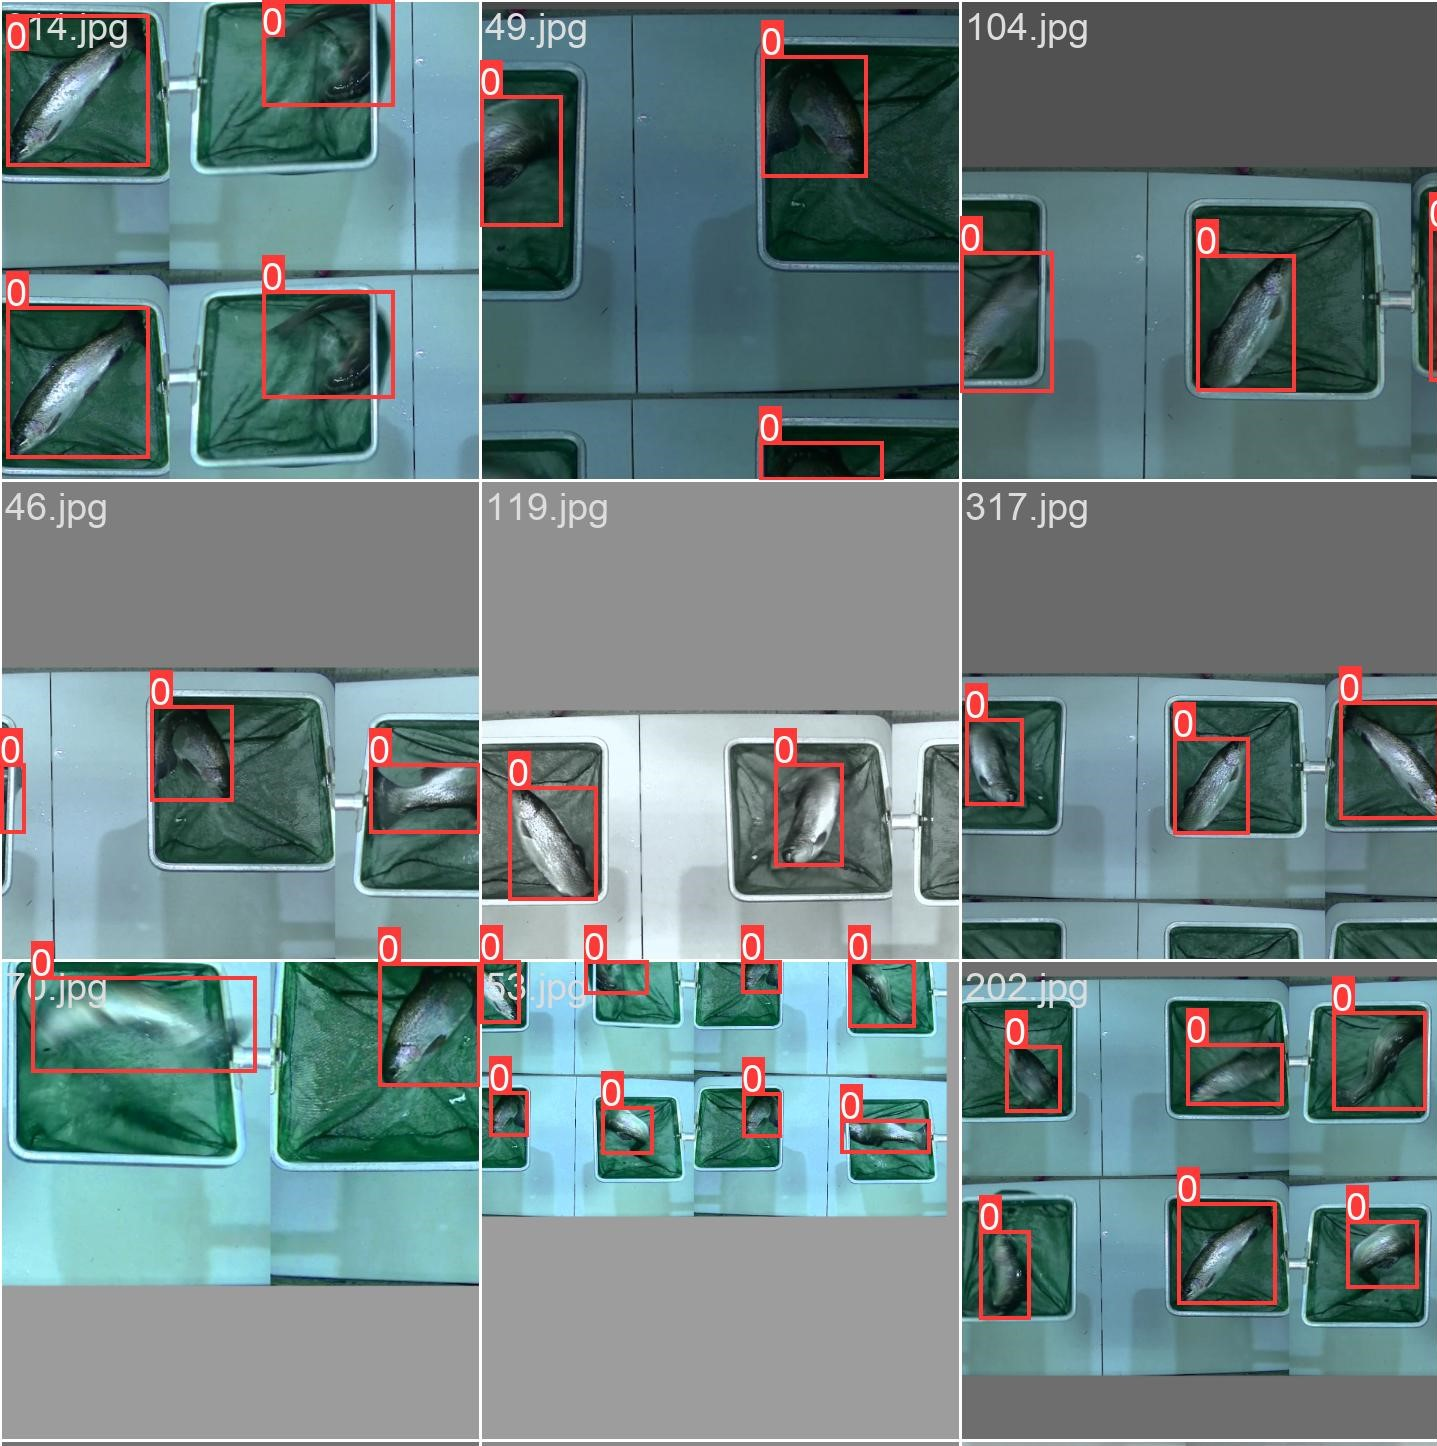
\includegraphics[width=0.7\textwidth]{images/13/a/EjemploAumento.jpg}
    \caption{Ejemplo de aumento de datos automático de \texttt{YOLO}}
    \label{fig:AumentoDatosYolo}
\end{figure}
\clearpage
Aparte de los posibles ajustes de hiperparámetros, es necesario explicar los estadísticos que se obtienen de realizar un entrenamiento con un modelo \texttt{YOLO}. En el caso de este trabajo, se realizará una 
explicación de los resultados que devuelve un modelo de detección.

Las métricas que se tienen en cuenta durante el entrenamiento son:

\begin{itemize}
    \item \textbf{Box Loss sobre el conjunto de entrenamiento}: representa el error del tamaño y posición de las \texttt{Bounding Boxes} de las etiquetas sobre las predichas en cada época. Cuando menor sea, 
    mayor es la cercanía entre las cajas predichas en el conjunto de entrenamiento respecto a sus etiquetas reales.\newline Una representación de un cálculo simple de este valor se puede ver en la \autoref{fig:IoU}, a través de la 
    intersección entre unidad, cuanto más cerca esté de 1, mejor.

    \begin{figure}[H]
        \centering
        \includegraphics[width=0.4\textwidth]{images/13/a/IoU.png}
        \caption{Factor IoU para calcular la perdida de cajas en una \texttt{CNN} de detección}
        \label{fig:IoU}
    \end{figure}

    \item \textbf{Cls Loss sobre el conjunto de entrenamiento}: representa el error de clasificación de cada objeto detectado en la imagen respecto al de la etiqueta real en el conjunto de entrenamiento.
    \item \textbf{Dfl Loss sobre el conjunto de entrenamiento}: es un error sobre la capacidad del modelo \texttt{YOLO} para soportar deformaciones de los objetos detectados.
    \item \textbf{Precisión (B)}: indica la precisión general sobre los objetos detectados, para realizar este cálculo se tienen en cuenta todas las métricas anteriores como una media con pesos y condiciones. Idealmente es 1 como máximo.
    \item \textbf{Recall (B)}: indica la capacidad que se ha tenido para detectar todas las instancias, se utiliza después para saber cuantos elementos detecta con una precisión determinada. Idealmente es 1.
    \item \textbf{Métrica \acrshort{map}50 (B)}: es una métrica sobre la precisión media en elementos con una intersección entre unidad de \texttt{0.5}. Esta métrica se puede entender como la capacidad de detección 
    en elementos fáciles de forma correcta. Es bastante representativa en el entrenamiento para saber si algo malo esta sucediendo.
    \item \textbf{Métrica \acrshort{map}50-95 (B)}: igual que antes, representa una media ponderada de precisión, pero en este caso de los elementos con una intersección entre unidad en el rango de \texttt{0.5} a 
    \texttt{0.95}. Podemos considerar esto como las detecciones dificiles y ajustadas a los resultados que esperamos.
    \item \textbf{Box Loss sobre el conjunto de validación}: igual que el \texttt{Box Loss} sobre el conjunto de entrenamiento, pero en este caso, al no variar el conjunto de validación, se va tomando como referencia 
    entre épocas para saber si el entrenamiento esta siendo correcto.
    \item \textbf{Cls Loss sobre el conjunto de validación}: igual que en la situación de entrenamiento pero como métrica entre épocas en un conjunto de datos invariante.
    \item \textbf{Dfl Loss sobre el conjunto de validación}: igual que en la situación de entrenamiento pero como métrica entre épocas en un conjunto de datos invariante para la precisión en deformación.
\end{itemize}

Estas métricas idealmente van acercándose a valores aceptables según pasan las épocas. Esto puede ser guardado al finalizar un entrenamiento de forma automática por parte de \texttt{YOLO} como se puede ver en el 
ejemplo de la \autoref{fig:ResultadosEjemplo} para 100 épocas.

\begin{figure}[H]
    \centering
    \includegraphics[width=0.7\textwidth]{images/13/a/results.png}
    \caption{Ejemplo de imagen de resultados resumidos por parte de \texttt{YOLO}}
    \label{fig:ResultadosEjemplo}
\end{figure}

Adicionalmente, \texttt{YOLO} produce resultados adicionales, que dependiendo del objetivo de la red, se buscará maximizar uno u otro:

\begin{itemize}
    \item \textbf{Matriz de confusión}: es una matriz como la de la \autoref{fig:MatrizEjemplo},que muestra el número de objetos detectados y su clasificación, si el objeto está correctamente clasificado será un verdadero positivo, si 
    se piensa que hay objeto, pero no hay, será falso positivo y si no se detecta, pero existe será falso negativo. Finalmente se tiene la situación de un verdadero negativo si no hay y no se detecta un objeto. Al ser un 
    estadístico de clasificación por naturaleza, no es el más apropiado para el análisis de resultados en detección de objetos, y menos cuando solo hay 1 clase de objetos.

    \begin{figure}[H]
        \centering
        \includegraphics[width=0.35\textwidth]{images/13/a/MatrizConfusiónEjemplo.png}
        \caption{Ejemplo de matriz de confusión en la medicina}
        \label{fig:MatrizEjemplo}
    \end{figure}

    \item \textbf{Curva de puntuación F1}: representa la puntuación F1, que se calcula a través de \begin{equation*}\text{Puntuación F1} = \frac{2*Precision*Recall}{Precision+Recall}\end{equation*} siendo el recall 
    calculado como: \begin{equation*}\text{Recall} = \frac{TP}{TP+FN}\end{equation*}. Cuando mayor área tenga bajo la curva mejor, porque significará que hay más verdaderos positivos en precisiones altas respecto a falsos.
    \item \textbf{Curva de precisión contra recall}: muestra la relación entre precisión y recall, mostrando una relación entre los valores seleccionados para seleccionar umbrales.
    \item \textbf{Curva de precisión}: refleja para cada valor de confianza de clasificación de elemento la precisión media de esa asignación. Cuanto más plana y cercana al 1 sea, mejor. Idealmente sería un escalón.
    \item \textbf{Curva de recall}: muestra para cada valor de confianza, el recall medio en ese valor. Idealmente es una línea horizontal en \texttt{y=1}.
\end{itemize}


\clearpage
\subsection*{ANEXO B: Datos de entrenamiento}
\label{subsec:B}
\subsubsection*{Entrenamiento 1}
\label{train:1}
\begin{itemize}
    \item \textbf{Fecha}: 9 de abril de 2024 (Prueba de concepto).
    \item \textbf{Descripción del conjunto de datos}: 24 imágenes seleccionadas manualmente del video \verb|23_NT_R1_J1_P1_2.mp4|. Conjunto dividido en 70-15-15 para los respectivos subconjuntos.
    \item \textbf{Resultados de entrenamiento}: En las siguientes figuras se observan  unos resultados que aparentan buenos  para ser un primer entrenamiento, pero debido al conjunto de datos con datos gran similares entre sí, en 
    situaciones de posiciones de trucha nuevas, se observó problemas en la precisión de la red. Aparte de esto se puede ajustar más ya que con 100 épocas vemos que se para cuando todavía hay una tendencia 
    descendente en el error en el conjunto de validación.
    
    \begin{figure}[H]
        \centering
        \includegraphics[width=0.9\textwidth]{images/13/b/1/PR.png}
        \caption{Gráficas de estadísticos finales del entrenamiento 1}
        \label{fig:Estadisticos1}
    \end{figure}
    \begin{figure}[H]
        \centering
        \includegraphics[width=0.9\textwidth]{images/13/b/1/results.png}
        \caption{Gráficas de evolución en épocas del entrenamiento 1}
        \label{fig:Resultados1}
    \end{figure}
\end{itemize}
\subsubsection*{Entrenamiento 2}
\label{train:2}
\begin{itemize}
    \item \textbf{Fecha}: 25 de abril de 2024
    \item \textbf{Descripción del conjunto de datos}: al conjunto del \hyperref[train:1]{entrenamiento de prueba} se le añadieron imágenes extra y situaciones con redes vacías. En total 50 imágenes en división 70-15-15 para los subconjuntos.
    \item \textbf{Resultados del entrenamiento}: A través del aumento de datos del conjunto y con el mismo número de épocas, se puede observar en la \autoref{fig:Estadisticos2} que hemos mejorado mucho el \texttt{recall} teniendo menos falsos positivos, 
    pero hemos perdido precisión en situaciones de poca confianza, esto puede ser debido al añadir imágenes de redes sin peces, pero no es nada problemático, ya que para \texttt{Bounding Boxes} con tan poca confianza, es mejor no procesarlas. 
    Aparte se ve en la \autoref{fig:Resultados2} que hemos mejorado mucho la precisión en la perdida de las \texttt{Bounding Boxes}, esto era el objetivo. Vemos que el resto de parametros no han cambiado mucho, buena señal.
    \begin{figure}[H]
        \centering
        \includegraphics[width=0.82\textwidth]{images/13/b/2/graficas2.png}
        \caption{Gráficas de estadísticos finales del entrenamiento 2}
        \label{fig:Estadisticos2}
    \end{figure}
    \begin{figure}[H]
        \centering
        \includegraphics[width=0.9\textwidth]{images/13/b/2/results.png}
        \caption{Gráficas de evolución en épocas del entrenamiento 2}
        \label{fig:Resultados2}
    \end{figure}
\end{itemize}
\subsubsection*{Entrenamiento 3}
\label{train:3}
\begin{itemize}
    \item \textbf{Fecha}: 4 de mayo de 2024
    \item \textbf{Descripción del conjunto de datos}: Mismo conjunto que el \hyperref[train:2]{entrenamiento anterior}
    \item \textbf{Resultados del entrenamiento}: a través del aumento de las épocas hasta 300, se pudo observar como se podían alcanzar valores de error en las \texttt{Bounding Boxes} bastante más bajas. 
    Este entrenamiento también dejo claro que el conjunto de datos de validación era demasiado reducido y no era suficientemente representativo, las imágenes eran muy similares entre sí.

    \begin{figure}[H]
        \centering
        \includegraphics[width=0.95\textwidth]{images/13/b/3/graficas2.png}
        \caption{Gráficas de estadísticos finales del entrenamiento 3}
        \label{fig:Estadisticos3}
    \end{figure}
    \begin{figure}[H]
        \centering
        \includegraphics[width=0.95\textwidth]{images/13/b/3/results.png}
        \caption{Gráficas de evolución en épocas del entrenamiento 3}
        \label{fig:Resultados3}
    \end{figure}
\end{itemize}
\clearpage
\subsubsection*{Entrenamiento 4}
\label{train:4}
\begin{itemize}
    \item \textbf{Fecha}: 4 de mayo de 2024
    \item \textbf{Descripción del conjunto de datos}: el conjunto de datos fue expandido con imágenes de los videos antiguos, obteniendo en total 84 imágenes representativas divididas en 70-15-15.
    \item \textbf{Resultados del entrenamiento}: por los nuevos tipos de imágenes añadidas, hemos perdido en la mayoría de métricas, pero esta red es mucho más representativa para los datos reales. 
    Además de esto, el conjunto de validación que se usa de referencia ahora es mucho más realista y tiene imágenes difíciles que implican movimientos, ya que para imágenes de truchas estáticas ha 
    estado funcionando correctamente durante todos los entrenamientos.
    
    \begin{figure}[H]
        \centering
        \includegraphics[width=0.9\textwidth]{images/13/b/4/graficas2.png}
        \caption{Gráficas de estadísticos finales del entrenamiento 4}
        \label{fig:Estadisticos4}
    \end{figure}
    \begin{figure}[H]
        \centering
        \includegraphics[width=0.9\textwidth]{images/13/b/4/results.png}
        \caption{Gráficas de evolución en épocas del entrenamiento 4}
        \label{fig:Resultados4}
    \end{figure}

\end{itemize}

\clearpage

\subsubsection*{Entrenamiento Final}
\label{train:final}
\begin{itemize}
    \item \textbf{Fecha}: 9 de junio de 2024
    \item \textbf{Descripción del conjunto de datos}: 203 imágenes en total. Se añadieron fotogramas aleatorios de varios videos del experimento \textit{NetTest} para poder manejar un conjunto más grande.
    \item \textbf{Resultados del entrenamiento}: resultados muy positivos, sobre todo en la \autoref{fig:ResultadosFinal} en la confianza con la que se realizan las clasificaciones y la curva F1, que aún siendo mejorable, solo tiene problemas 
    con falsos positivos en valores de confianza muy altos. Aparte de esto, como se puede apreciar en la \autoref{fig:EstadisticosFinal}, el error de aproximación a la \texttt{Bounding Box} predicha se ha 
    conseguido reducir mucho tanto en entrenamiento como en el conjunto de validación, que es principalmente lo que se necesitaba del modelo \texttt{YOLO} para este trabajo.
    
    \begin{figure}[H]
        \centering
        \includegraphics[width=0.9\textwidth]{images/13/b/final/graficas2.png}
        \caption{Gráficas de estadísticos del último entrenamiento}
        \label{fig:EstadisticosFinal}
    \end{figure}
    \begin{figure}[H]
        \centering
        \includegraphics[width=0.9\textwidth]{images/13/b/final/results.png}
        \caption{Gráficas de evolución en épocas del último entrenamiento}
        \label{fig:ResultadosFinal}
    \end{figure}
\end{itemize}

\clearpage

\subsubsection*{Entrenamiento OBB}
\label{OBB:1}
\begin{itemize}
    \item \textbf{Fecha}: 9 de mayo de 2024
    \item \textbf{Descripción del conjunto de datos}: conjunto común al \hyperref[train:4]{entrenamiento 4}, 84 imágenes tanto de videos nuevos como de videos antiguos.
    \item \textbf{Resultados del entrenamiento}: se observan los problemas que conllevan trabajar con \texttt{Bounding Boxes} orientadas, se pierde mucho tanto en métricas como en rendimiento general. 
    El punto positivo de este sistema es acotar lo máximo posible la \texttt{Bounding Box} al elemento, pero principalmente se observa una dificultad añadida y necesidad de mucho más entrenamiento y 
    ajuste de hiperparámetros para conseguir sobre todo mejorar el \acrshort{map}50-95.

    \begin{figure}[H]
        \centering
        \includegraphics[width=0.9\textwidth]{images/13/b/obb/graficas2.png}
        \caption{Gráficas de estadísticos finales del entrenamiento \texttt{OBB}}
        \label{fig:EstadisticosOBB}
    \end{figure}
    \begin{figure}[H]
        \centering
        \includegraphics[width=0.9\textwidth]{images/13/b/obb/results.png}
        \caption{Gráficas de evolución en épocas del entrenamiento \texttt{OBB}}
        \label{fig:ResultadosOBB}
    \end{figure}

\end{itemize}

\end{document}